% CVSId: $Id: Example.tex,v 1.1.1.1 2000/11/28 11:15:12 exupery Exp $
\documentclass[%
xcolor=pdftex,dvipsnames,table%,
%pdf,
%nocolorBG,
%colorBG,
%slideColor,
%slideBW,
%draft,
%frames
%azure
%contemporain
%nuancegris
%troispoints
%lignesbleues
%darkblue
%alienglow
%autumn
%10pt
]{beamer}
%%%%%%%%%%%%%%%%%%%%%%%%%%%%%%
%Force pdflatex processing even with "$ latex" (required by arXiv)
\pdfoutput=1
%%%%%%%%%%%%%%%%%%%%%%%%%%%%%
\mode<presentation>
{
  \usetheme{Madrid}
  % or ...
%%%%%%%%%%%%%%%%%%%%%%%%%%%%%%%%%%%%%
%para revelar texto a aparecer en overlays
  \setbeamercovered{transparent} 
  %\setbeamercovered{invisible}
%%%%%%%%%%%%%%%%%%%%%%%%%%%%%%%%%%%%%
  \setbeamertemplate{blocks}[rounded][shadow=true]
  \setbeamertemplate{navigation symbols}{}

  \setbeamertemplate{footline}{%\hspace*{.5cm}
    \scriptsize{\phantom{Gg}%\insertauthor 
      \hspace*{50pt} 
      \hfill \insertframenumber
      \hspace*{.5cm}}}

  % or whatever (possibly just delete it)
  %\useoutertheme{shadow} 
}
\graphicspath{{figures/}}
\usepackage[T1]{fontenc}
\usepackage[utf8]{inputenc}
\usepackage[spanish]{babel}
\spanishdecimal{.}
\usepackage{beamerprosper}
\usepackage{amsmath,amssymb}
\usepackage{graphicx}
\usepackage{mycolors}
\usepackage{xmpmulti}
\usepackage{multimedia}
\usepackage{siunitx} 
\sisetup{group-minimum-digits=4} %compatibility with PDG

\usepackage{comment}
\includecomment{comentar}
\specialcomment{comentar}
{\begingroup}{\medskip\endgroup}
\excludecomment{comentar}

\includecomment{comentario}
\specialcomment{comentario}
{\begingroup}{\endgroup}
\excludecomment{comentario}


\newcommand{\widescreen}{
\setlength{\paperwidth}{171 mm}
\setlength{\paperheight}{96 mm}
\setlength{\textwidth}{161 mm}
\setlength{\textheight}{86 mm}
}

%\widescreen


\title[ED] % (optional, use only with long paper titles)
{Interacciones fundamentales}

%\subtitle
%{Reconstruction of the neutrino mass matrix} % (optional)

\author[GFIF]% (optional, use only with lots of authors)
{Diego Restrepo\inst{1} }
% - Use the \inst{?} command only if the authors have different
%   affiliation.

\institute[UdeA] % (optional, but mostly needed)
{
  \inst{1}%
Instituto de F\'\i sica\\
Universidad de Antioquia
}
% - Use the \inst command only if there are several affiliations.
% - Keep it simple, no one is interested in your street address.

\date[] % (optional)
{
\hspace{-1.5cm}
\includegraphics[scale=0.4]{gfif_logo}\hspace{1cm} 
\includegraphics[scale=0.3]{udea}}


\subject{Talks}
% This is only inserted into the PDF information catalog. Can be left
% out. 



% If you have a file called "university-logo-filename.xxx", where xxx
% is a graphic format that can be processed by latex or pdflatex,
% resp., then you can add a logo as follows:

% \pgfdeclareimage[height=0.5cm]{university-logo}{university-logo-filename}
% \logo{\pgfuseimage{university-logo}}



% Delete this, if you do not want the table of contents to pop up at
% the beginning of each subsection:
%\AtBeginSubsection[]
%{
%  \begin{frame}<beamer>
%    \frametitle{Outline}
%    \tableofcontents[currentsection,currentsubsection]
%  \end{frame}
%}

\newcommand{\chml}[2]{$\underline{\text{#1\hspace{#2}}}$}
\begin{document}


%===============
\begin{comentar}
%===============  
%=============
\end{comentar}
%=============

\begin{frame}
  \titlepage
\end{frame}

%%%%%%%%%%%%%%%%%%

{
\usebackgroundtemplate{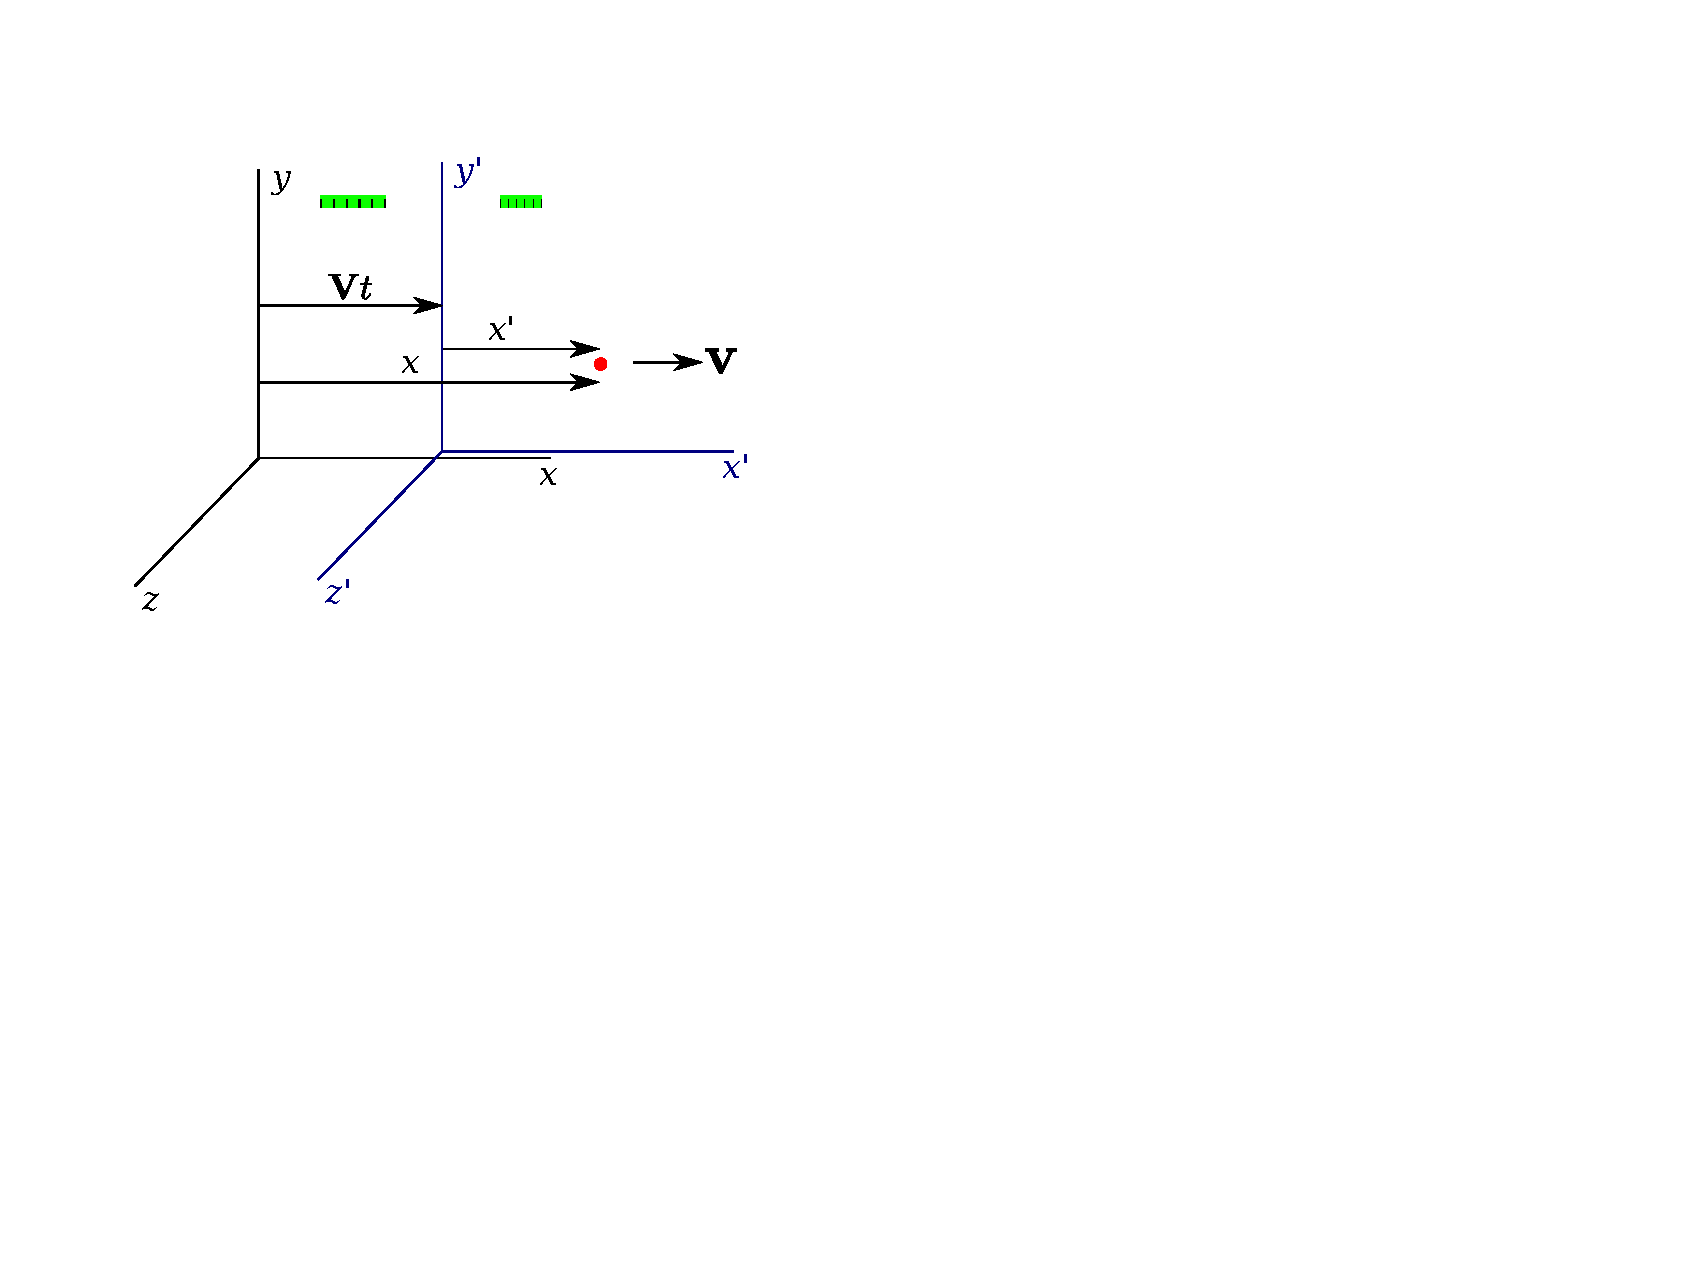
\includegraphics[width=\paperwidth]{lorentz1}}
%\setbeamercovered{invisible}
\begin{frame}[plain]
\qquad

\vspace{6cm}
\begin{center}
  Principio de relatividad+Homogeneidad+Isotropía

  $\Downarrow$

    Existencia de velocidad límite
\end{center}
\end{frame}
}


\begin{frame}
  \begin{columns}
    \begin{column}{0.5\linewidth}
        \begin{block}{Regla de adición de velocidades}
    \begin{itemize}
    \item  la velocidad relativa entre dos objetos moviéndose a la velociad límite,  es la velocidad límite.
    \item Todos los observadores ven moverse un objeto a la velocidad límite si dicho onjeto se mueve a la velocidad límite. 
    \end{itemize}
  \end{block}
    \end{column}
    \begin{column}{0.6\linewidth}
      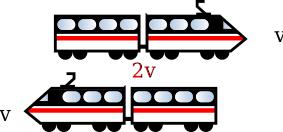
\includegraphics[scale=0.7]{train}

\hrulefill{}

\vspace{1cm}

      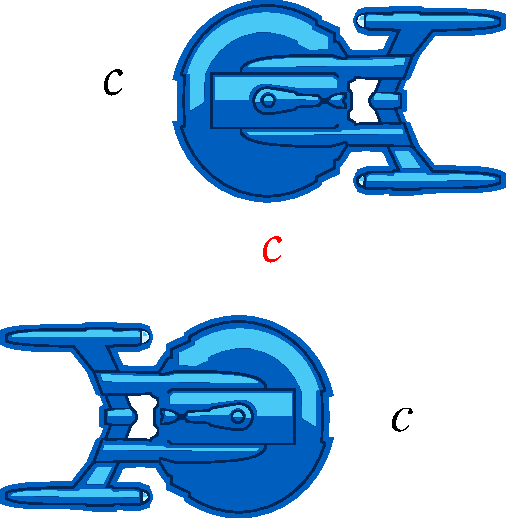
\includegraphics[scale=0.5]{Enterprise}

    \end{column}
  \end{columns}
%dibujar dos metros
%dibujar un par de naves enterprise comparada 
\end{frame}


% %%%%%%%%%%%%%%%%%%%%%%%%%%%%%%%%%%%%
{
\usebackgroundtemplate{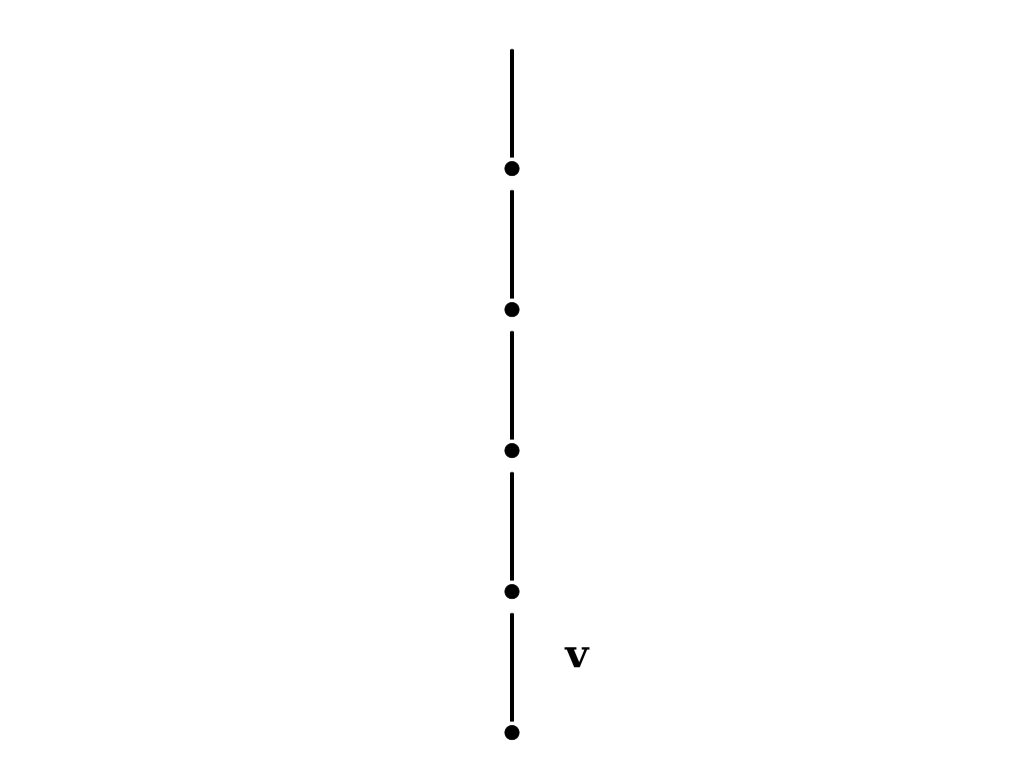
\includegraphics[width=\paperwidth]{uniform}}
%\setbeamercovered{invisible}
\begin{frame}[plain]
  \begin{flushleft}
\textbf{Interacciones}

Cambio en la cantidad de\\
 movimiento

 \begin{align*}
   \mathbf{p}=&\gamma m \mathbf{v} &&&&
 \end{align*}
donde
\begin{align*}
  \gamma=\frac{1}{\sqrt(1-v^2/c^2)} &&&&
\end{align*}

\begin{align*}
  c=\SI{299 792 458}{ms^{-1}} & &&&&
\end{align*}
  \end{flushleft}
\end{frame}
}
% %%%%%%%%
% %%%%%%%%%%%%%%%%%%%%%%%%%%%%%%%%%%%%
% {
% \usebackgroundtemplate{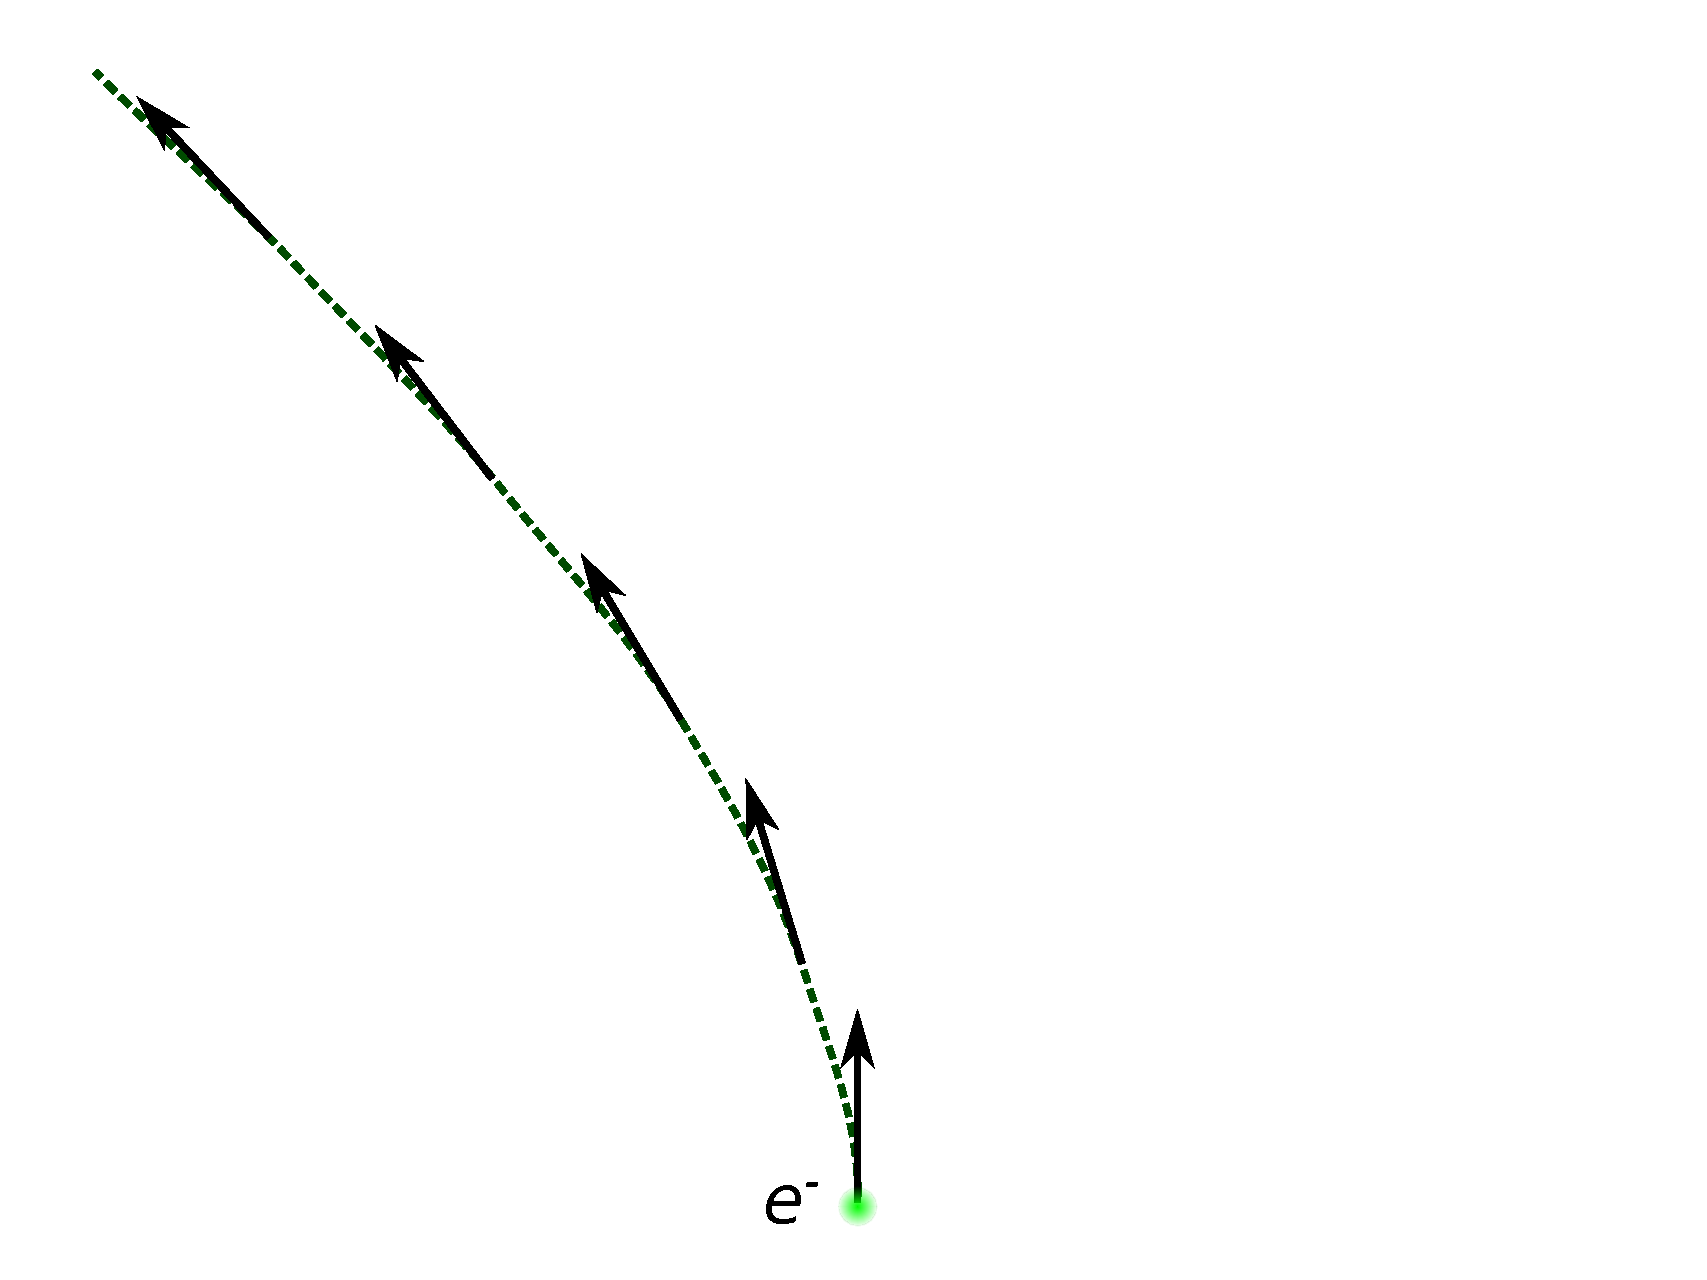
\includegraphics[width=\paperwidth]{repulsion1}}
% %\setbeamercovered{invisible}
% \begin{frame}[plain]
% \end{frame}
% }
% %%%%%%%%%%%%%%%%%%%%%%%%%%%%%%%%%%%%
% {
% \usebackgroundtemplate{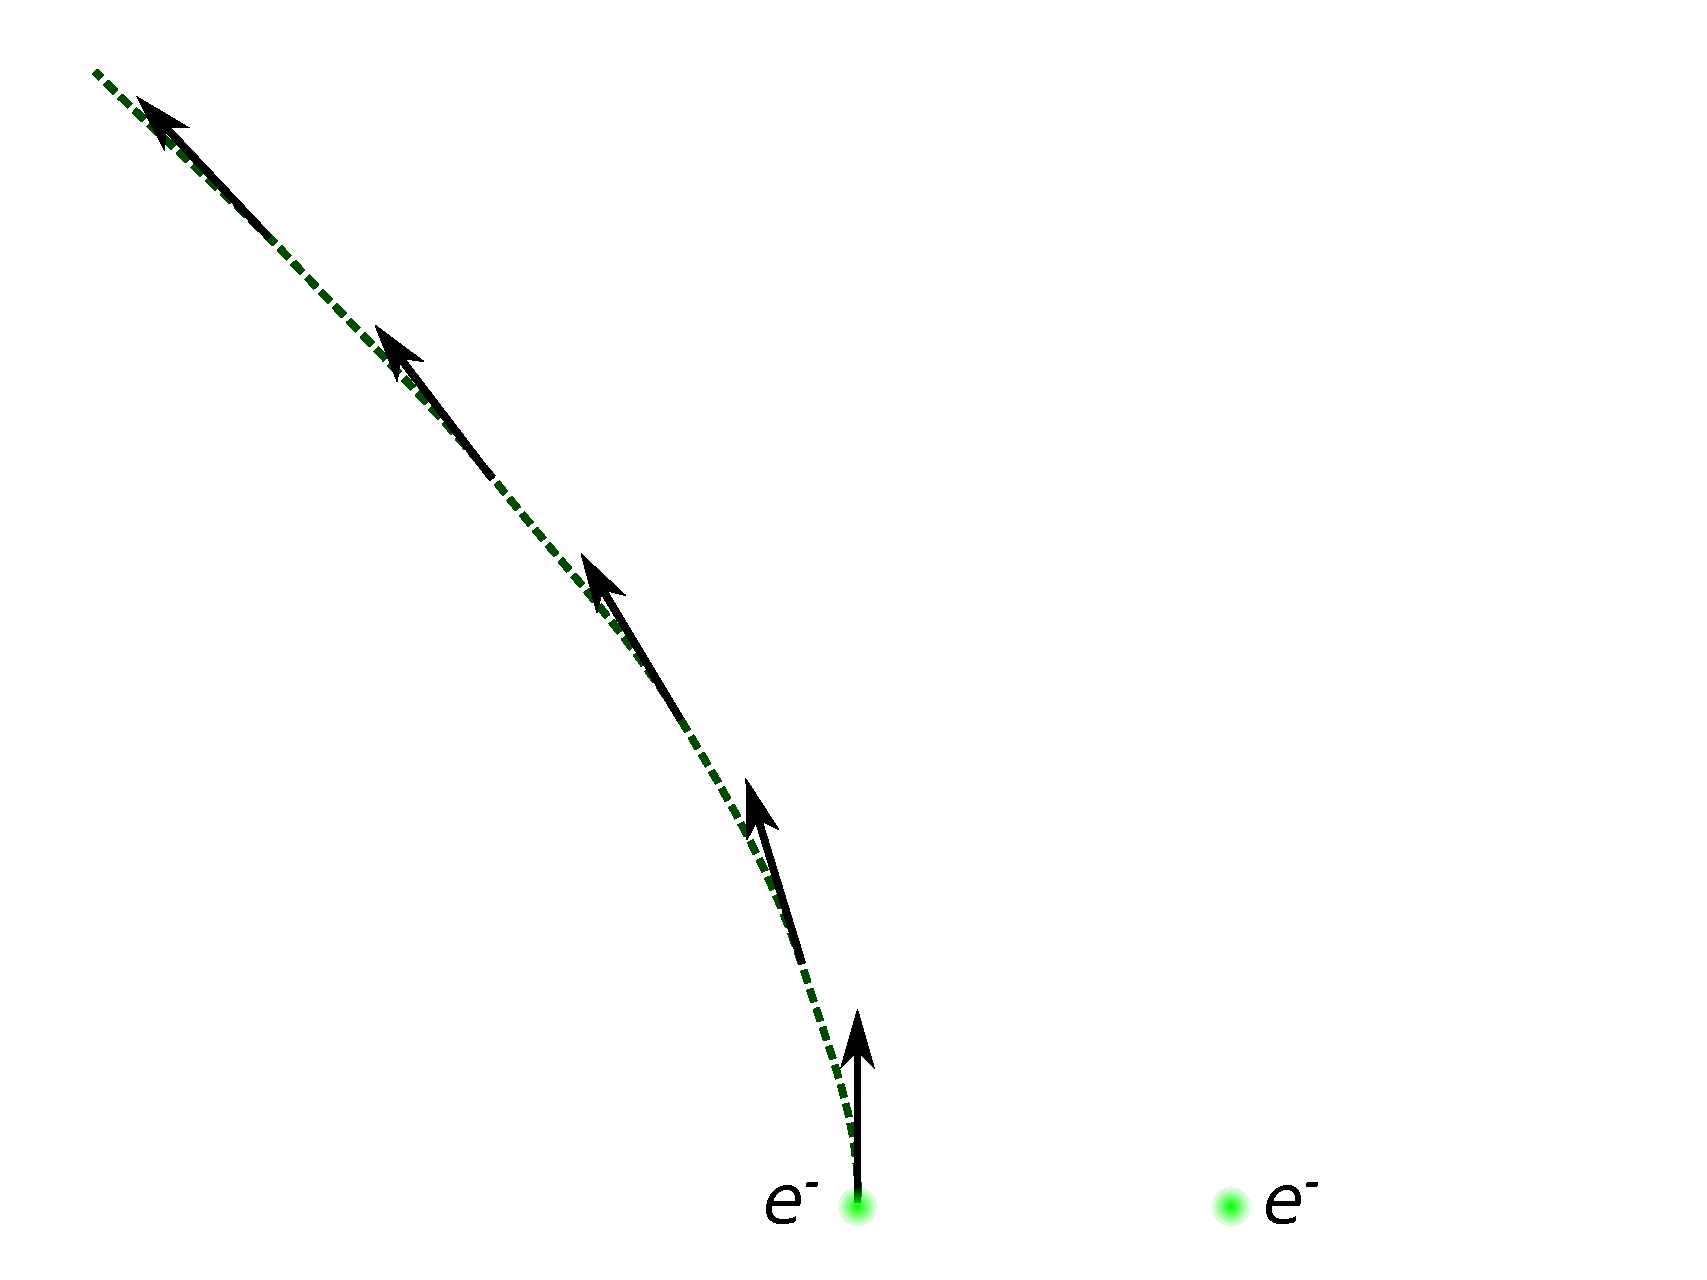
\includegraphics[width=\paperwidth]{repulsion2}}
% %\setbeamercovered{invisible}
% \begin{frame}[plain]
% \end{frame}
% }
% %%%%%%%%%%%%%%%%%%%%%%%%%%%%%%%%%%%%
% {
% \usebackgroundtemplate{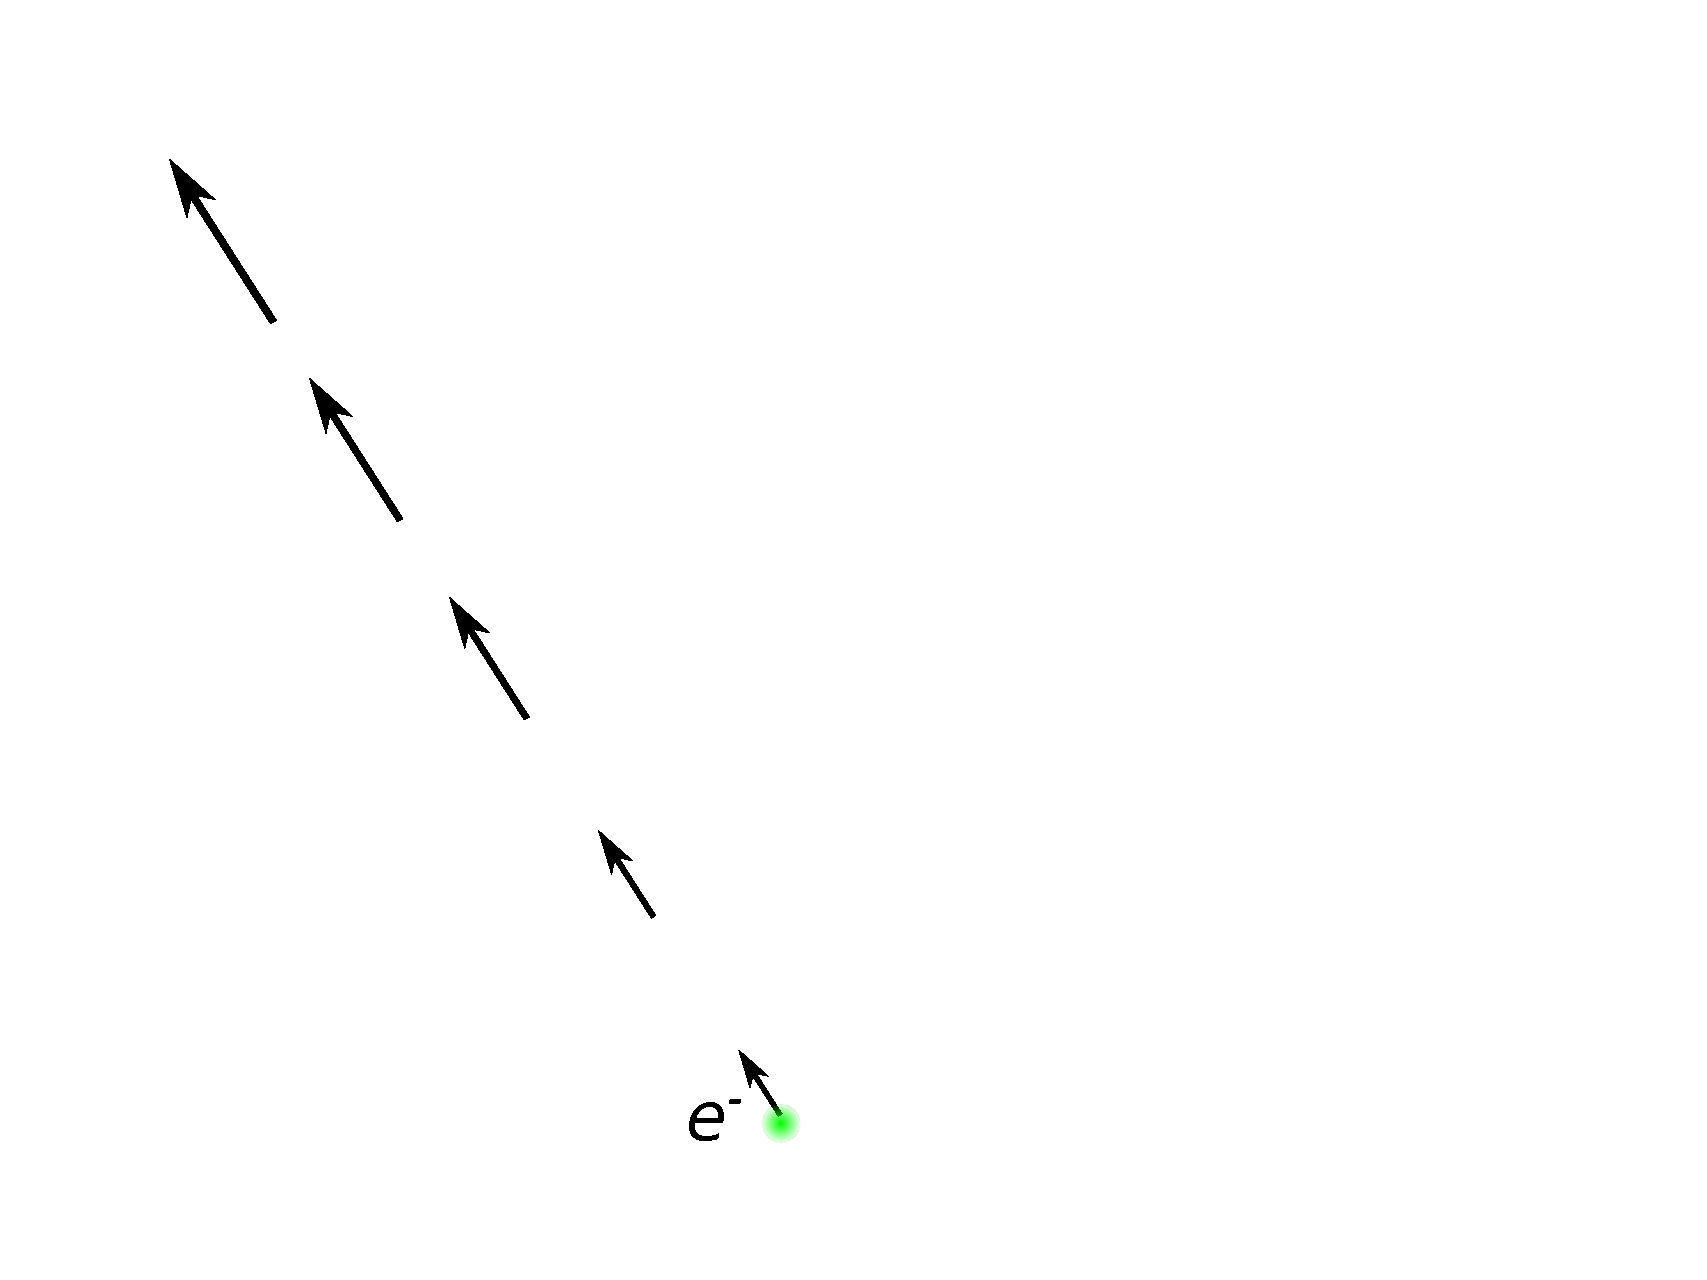
\includegraphics[width=\paperwidth]{repulsion3}}
% %\setbeamercovered{invisible}
% \begin{frame}[plain]
% \end{frame}
% }
% %%%%%%%%%%%%%%%%%%%%%%%%%%%%%%%%%%%%
% {
% \usebackgroundtemplate{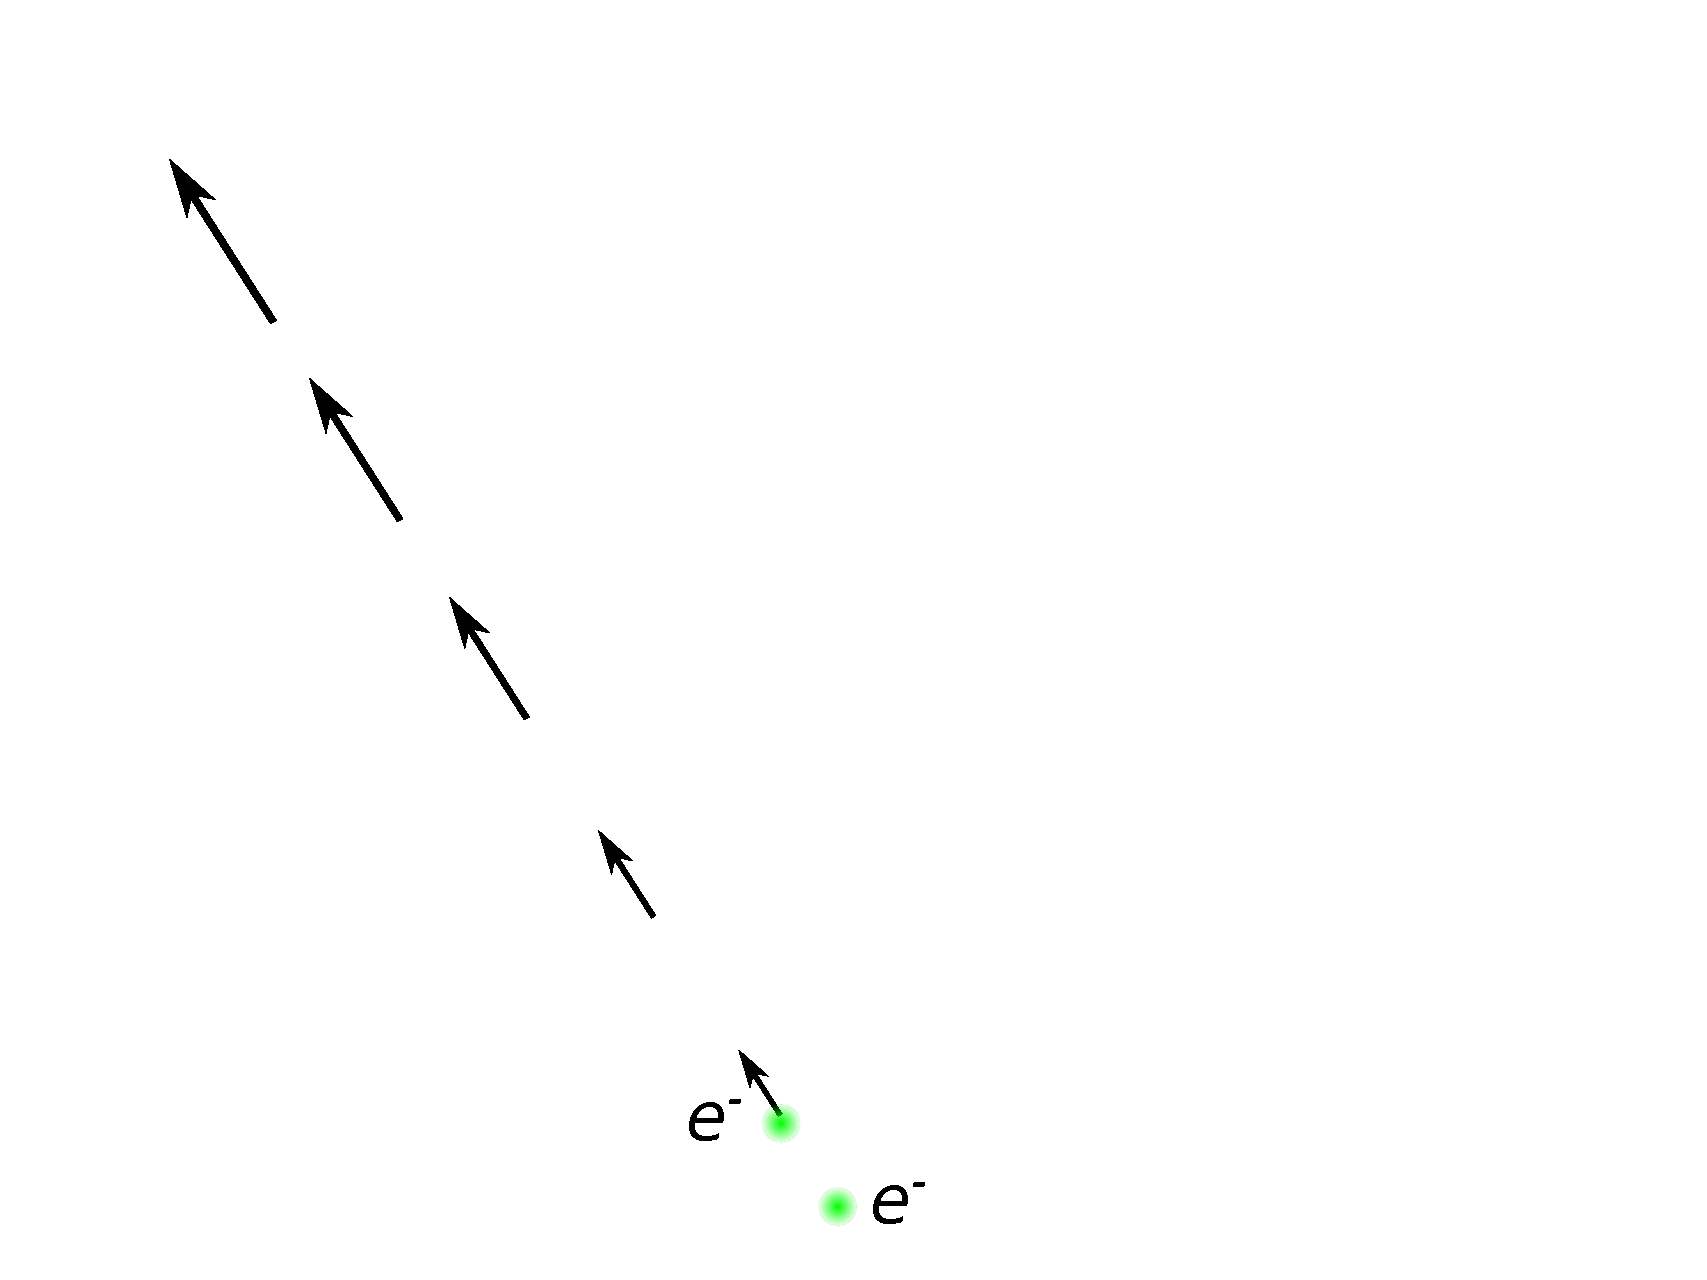
\includegraphics[width=\paperwidth]{repulsion4}}
% %\setbeamercovered{invisible}
% \begin{frame}[plain]
% \end{frame}
% }
%%%%%%%%%%%%%%%%%%%%%%%%%%%%%%%%%%%%%%%%
\begin{frame}{Teorema de Noether}
  Por cada \alert{simetría} de la naturaleza hay una \alert{cantidad que se conserva}.

  \begin{flushright}
    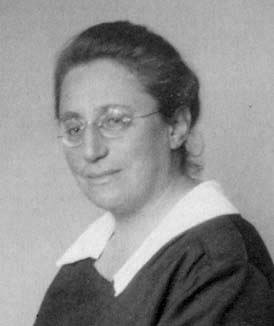
\includegraphics[scale=0.35]{Noether}\\
    Emmy Noether (1882-1935)
  \end{flushright}
\end{frame}
%%%%%%%%%%%%%%%%%%%%%%%%%%%%%%%%%%%%
\begin{frame}{Simetrías externas}
\rowcolors{1}{RoyalBlue!20}{}
\begin{tabular}{p{0.5\textwidth}p{0.5\textwidth}}
  Simetría  & Cantidad conservada\\
  Las leyes de la física no cambian con el tiempo & Energía\\
  Las leyes de la física son las mismas en todas partes & Cantidad de movimiento.
\end{tabular}
\end{frame}
\begin{frame}
  Por cada smetría \alert{local} hay alguna partícula \alert{sin masa}
\end{frame}

\begin{frame}[plain]
    El Grupo de Galileo es un grupo de Lie que incluye
    \begin{columns}
      \column{.48\textwidth}
      \begin{block}<1->{}
              \begin{itemize}
      \item Traslaciones temporales
\vspace{-0.3cm}
      \begin{align*}
        t&\to t+\tau\\
        \mathbf{x}&\to \mathbf{x}
      \end{align*}

\vspace{-0.3cm}
    \item Traslaciones espaciales
\vspace{-0.3cm}
      \begin{align*}
        t&\to t\\
        \mathbf{x}&\to \mathbf{x}+\mathbf{a}
      \end{align*}

\vspace{-0.3cm}
    \item Impulsos
\vspace{-0.3cm}
      \begin{align*}
        t&\to t\\
        \mathbf{x}&\to \mathbf{x}+\mathbf{v}t
      \end{align*}

\vspace{-0.3cm}
    \item Rotaciones
\vspace{-0.3cm}
      \begin{align*}
        t&\to t\\
        \mathbf{x}&\to \mathbf{x}+\mathbf{R}x
      \end{align*}
    $\mathbf{R}$ una matriz ortogonal
    \end{itemize}
      \end{block}
\column{.48\textwidth}
\begin{block}<2->{}
Conservación de la Energía

\vspace{1cm}

  Conservación del momento

\vspace{1.3cm}

Movimiento uniforme del centro de masa
\vspace{1cm}

Conservación del momento angular

\vspace{1cm}
\qquad
\end{block}
    \end{columns}
\end{frame}
\begin{frame}
  \begin{block}{Grupos}
    Considere $x,y,z\in G$ 

    ``*'': cualquier regla que combine los objetos en $G$
    \begin{itemize}
    \item Clausura: $z=x*y\in G$
    \item Asociatividad: $z*(x*y)=(z*x)*y$
    \item Identidad: $\exists I$ t.q $I*x=x$
    \item Inverso: $\exists x'$ t.q $x*x'=I$
    \end{itemize}
  \end{block}
  \begin{example}
    \begin{itemize}
    \item El conjunto de enteros bajo la adición
    \end{itemize}
  \end{example}
\end{frame}
\begin{frame}[plain]
  \begin{block}{Grupos de Lie}
    Informalmente es un grupo de simetrías donde las simetría son continuas

    Formalmente, un Grupo de Lie es un Grupo que también un espacio matemático que localmente es lo suficientemente general a un espacio euclidiano como para permitir hacer cálculo diferencial.
  \end{block}
  \begin{example}
    Conjunto de números reales bajo la adición
  \end{example}
\end{frame}

%%%%%%%%%%%%%%%%%%%%%%%%%%%


\begin{frame}[plain]
  \begin{block}{Grupo de Lorentz}
    \begin{itemize}
    \item     Es un grupo de Lie que incluye además de las traslaciones espaciales, traslaciones temporales y rotaciones a  las transformaciones de Lorentz. 

Es el único grupo compatible con el principio de relatividad que no genera paradojas (conocidas)


\item Las ecuaciones de Maxwell nacieron invariates bajo transformaciones de Lorentz.
  
\end{itemize}
  \end{block}
  \begin{block}{Libertad gauge}
\begin{itemize}
\item Los campos electromagnéticos también son invariantes bajo transformaciones gauge:

Si $A(x)$ representa la energía potencial del campo de fuerza en cada punto $x$ en el espacio. Si uno cambia $A(x)$ por otra función en la forma dictada por la transformación gauge, está nueva función sigue describiendo el \emph{mismo} campo de fuerza electromagnético. 

La libertad para escoger la función de energía potencial de un campo se llama libertad gauge.

    \end{itemize}
Qué ley de conservación esta asociada a esta simetría?
  \end{block}
\end{frame}

\begin{frame}
  \frametitle{Campos}
  \url{https://www.youtube.com/watch?v=GHtAwQXVsuk}
\end{frame}

\begin{frame}
  \frametitle{Radiación débil}
  600 millones de millones ne neutrinos provenientes del sol atraviesan cada segundo nuestro cuerpo, cuyo contenido en Postasio 40 emite 10000 millones de neutrinos cada segundo.
\end{frame}
%%%%%%%%%%%%%%%%%%%%%%%%%%%%%%%%%%%%
{
\usebackgroundtemplate{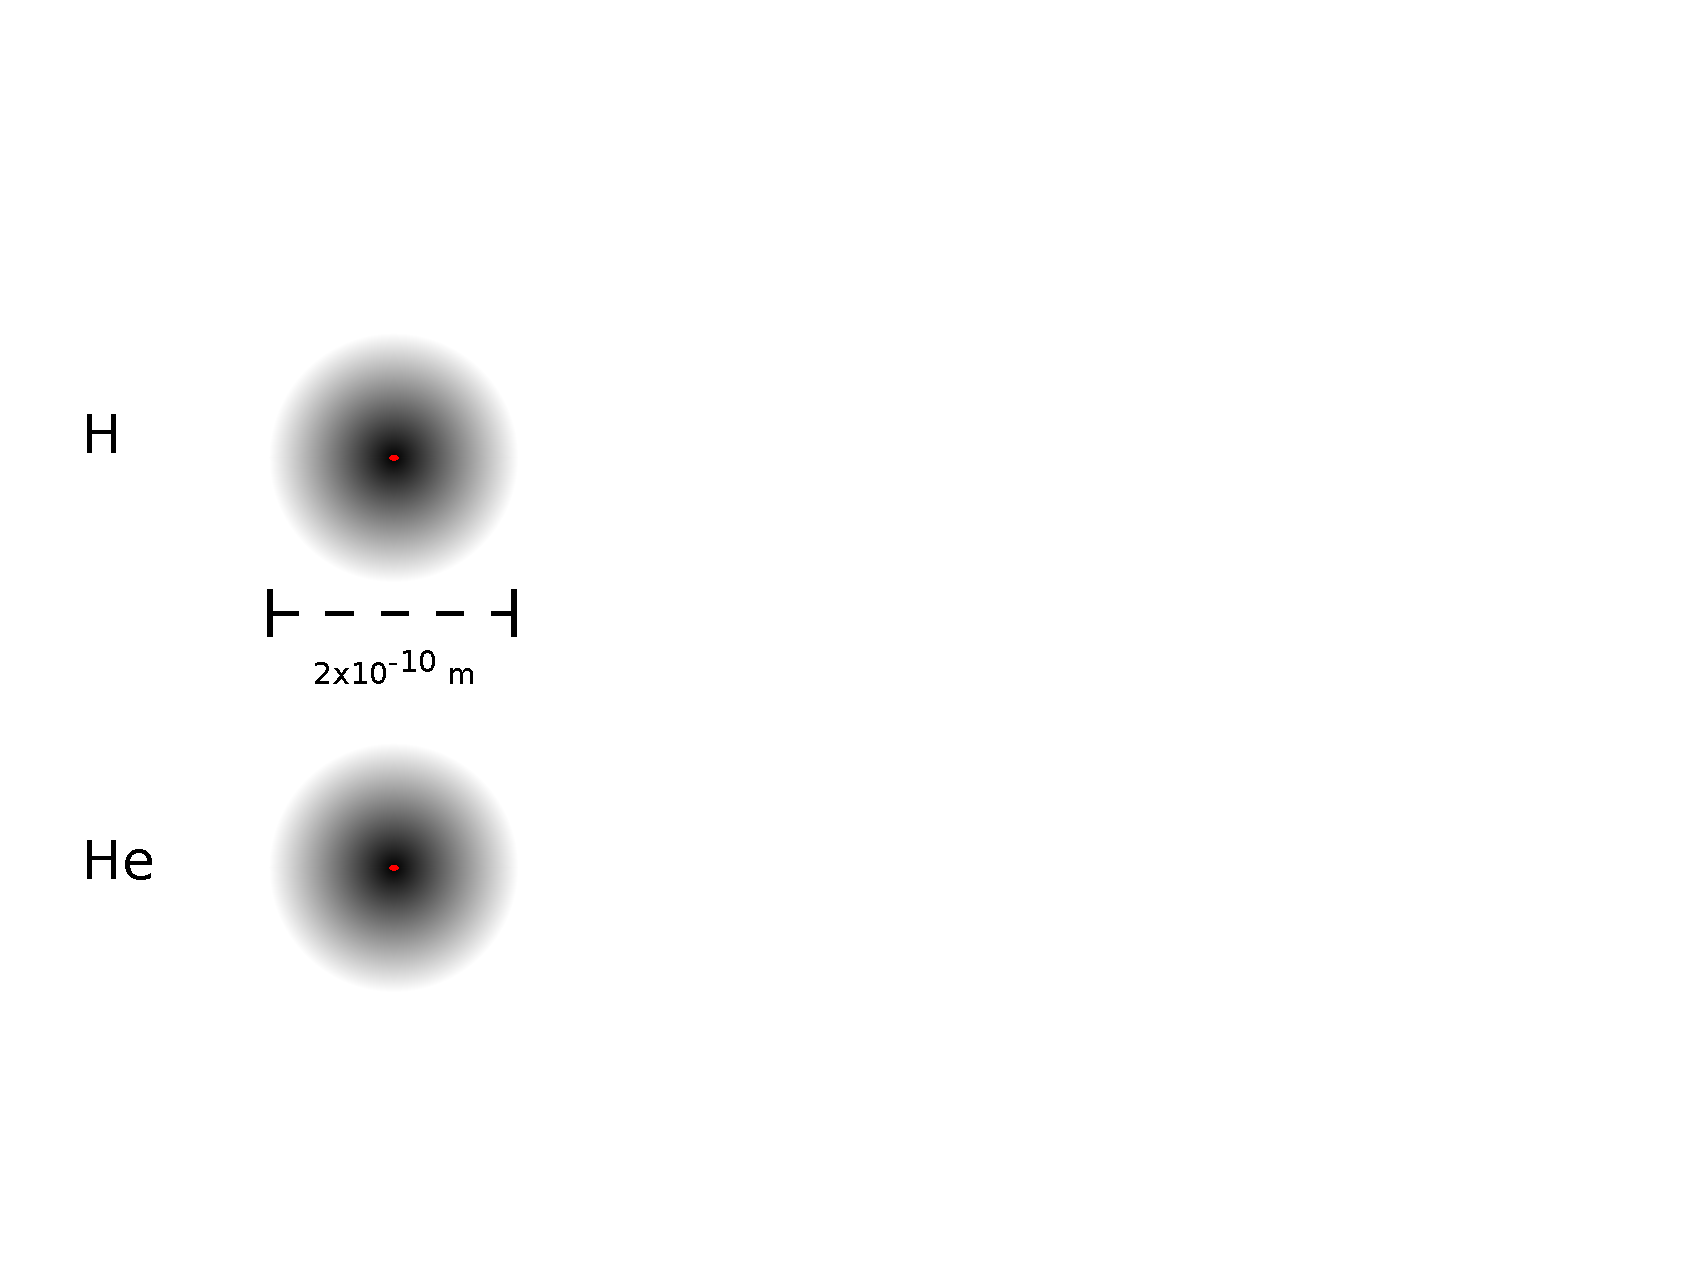
\includegraphics[width=\paperwidth]{interactions1}}
%\setbeamercovered{invisible}
\begin{frame}[plain]
\end{frame}
}
%%%%%%%%%%%%%%%%%%%%%%%%%%%%%%%%%%%%
{
\usebackgroundtemplate{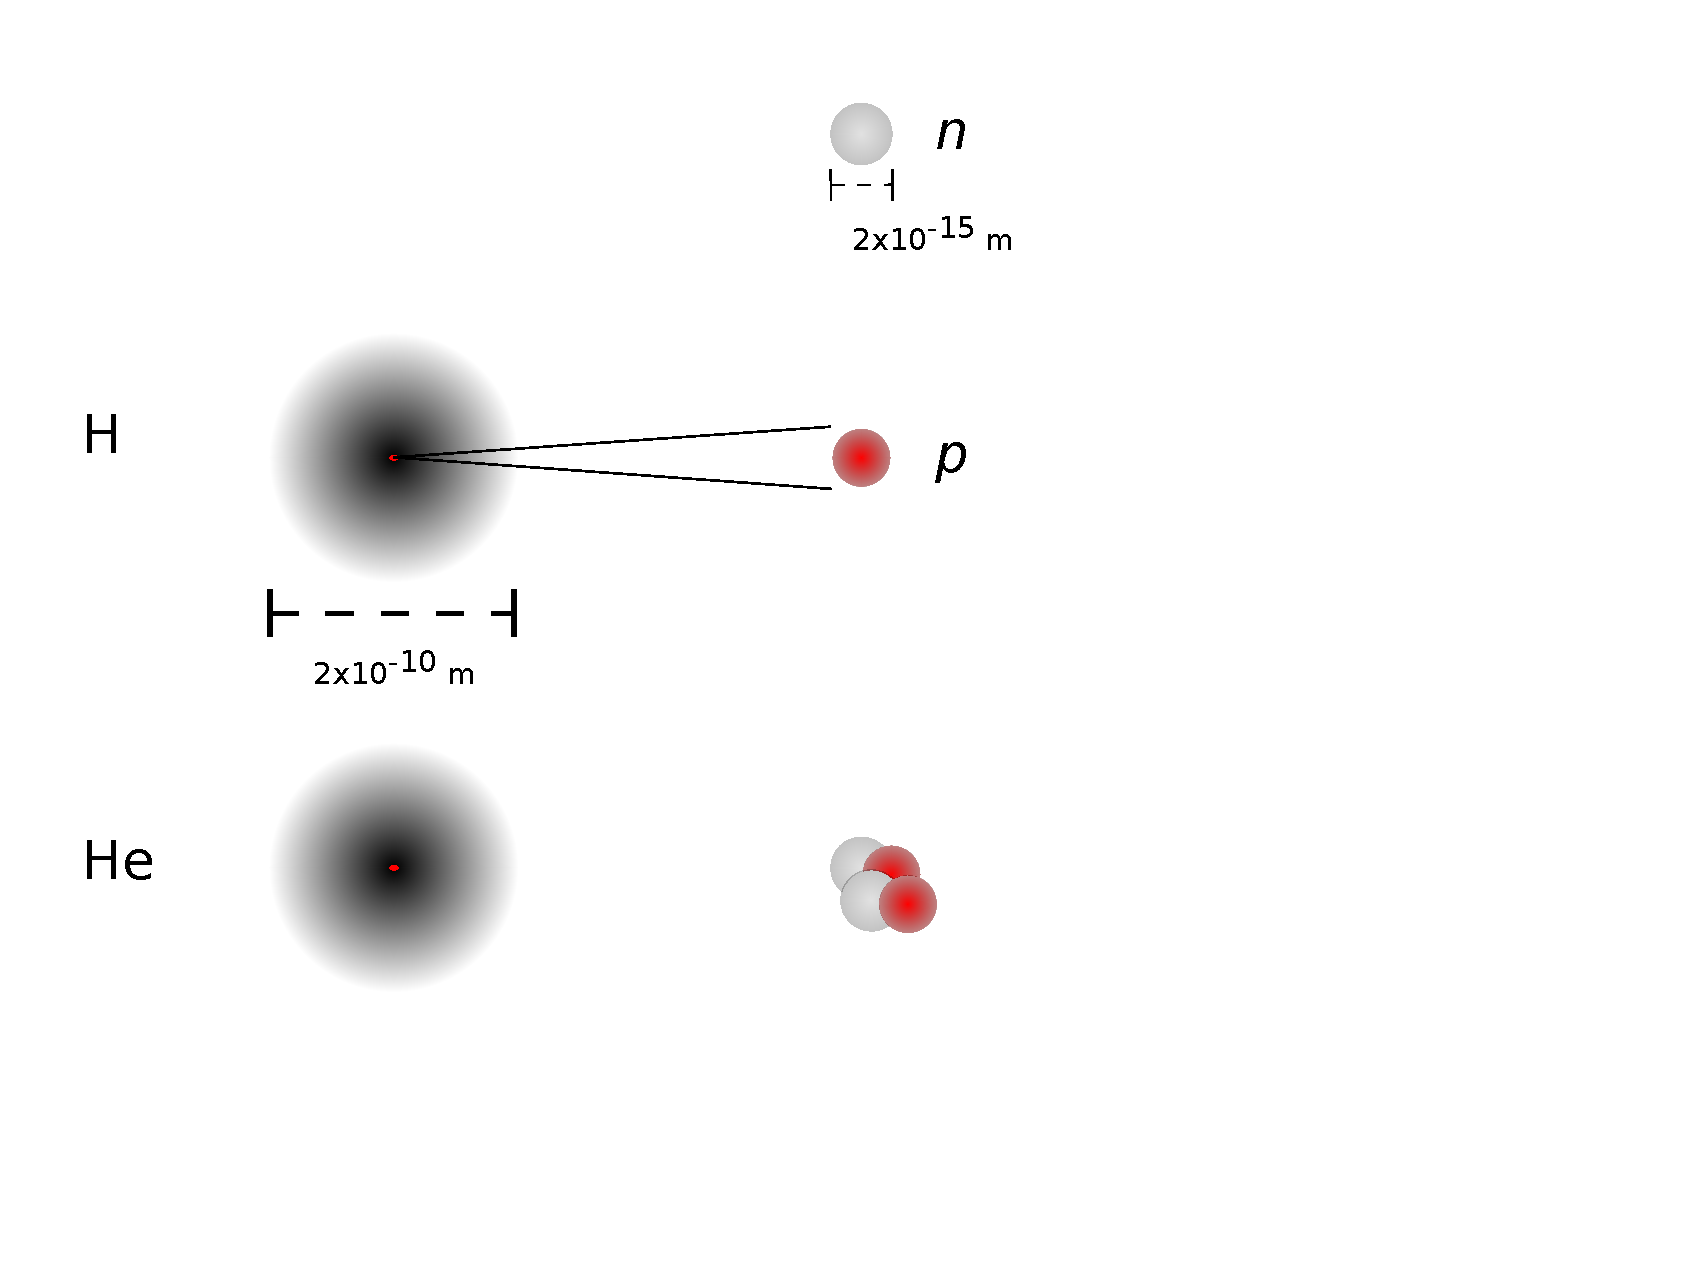
\includegraphics[width=\paperwidth]{interactions2}}
%\setbeamercovered{invisible}
\begin{frame}[plain]
\end{frame}
}
%%%%%%%%%%%%%%%%%%%%%%%%%%%%%%%%%%%%
{
\usebackgroundtemplate{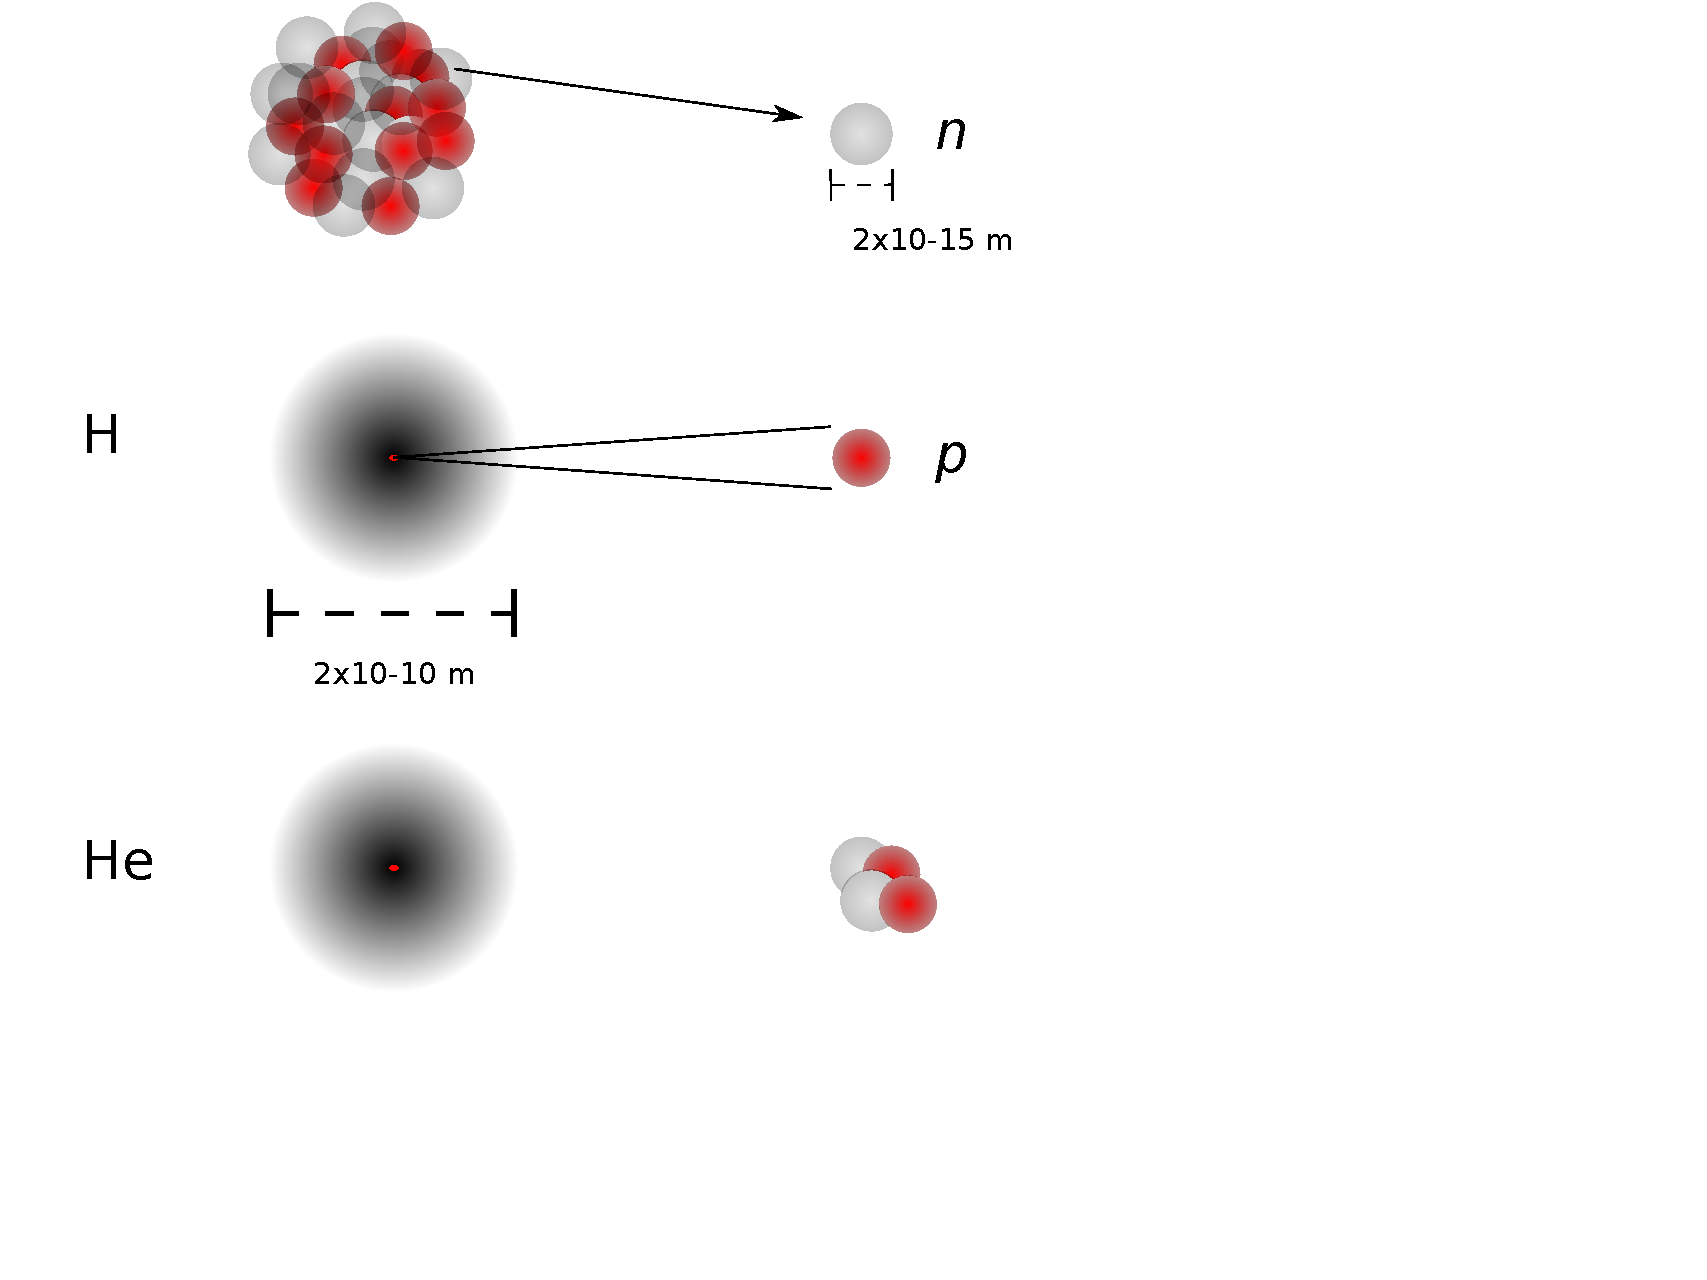
\includegraphics[width=\paperwidth]{interactions2a}}
%\setbeamercovered{invisible}
\begin{frame}[plain]
\end{frame}
}
%%%%%%%%%%%%%%%%%%%%%%%%%%%%%
{
\usebackgroundtemplate{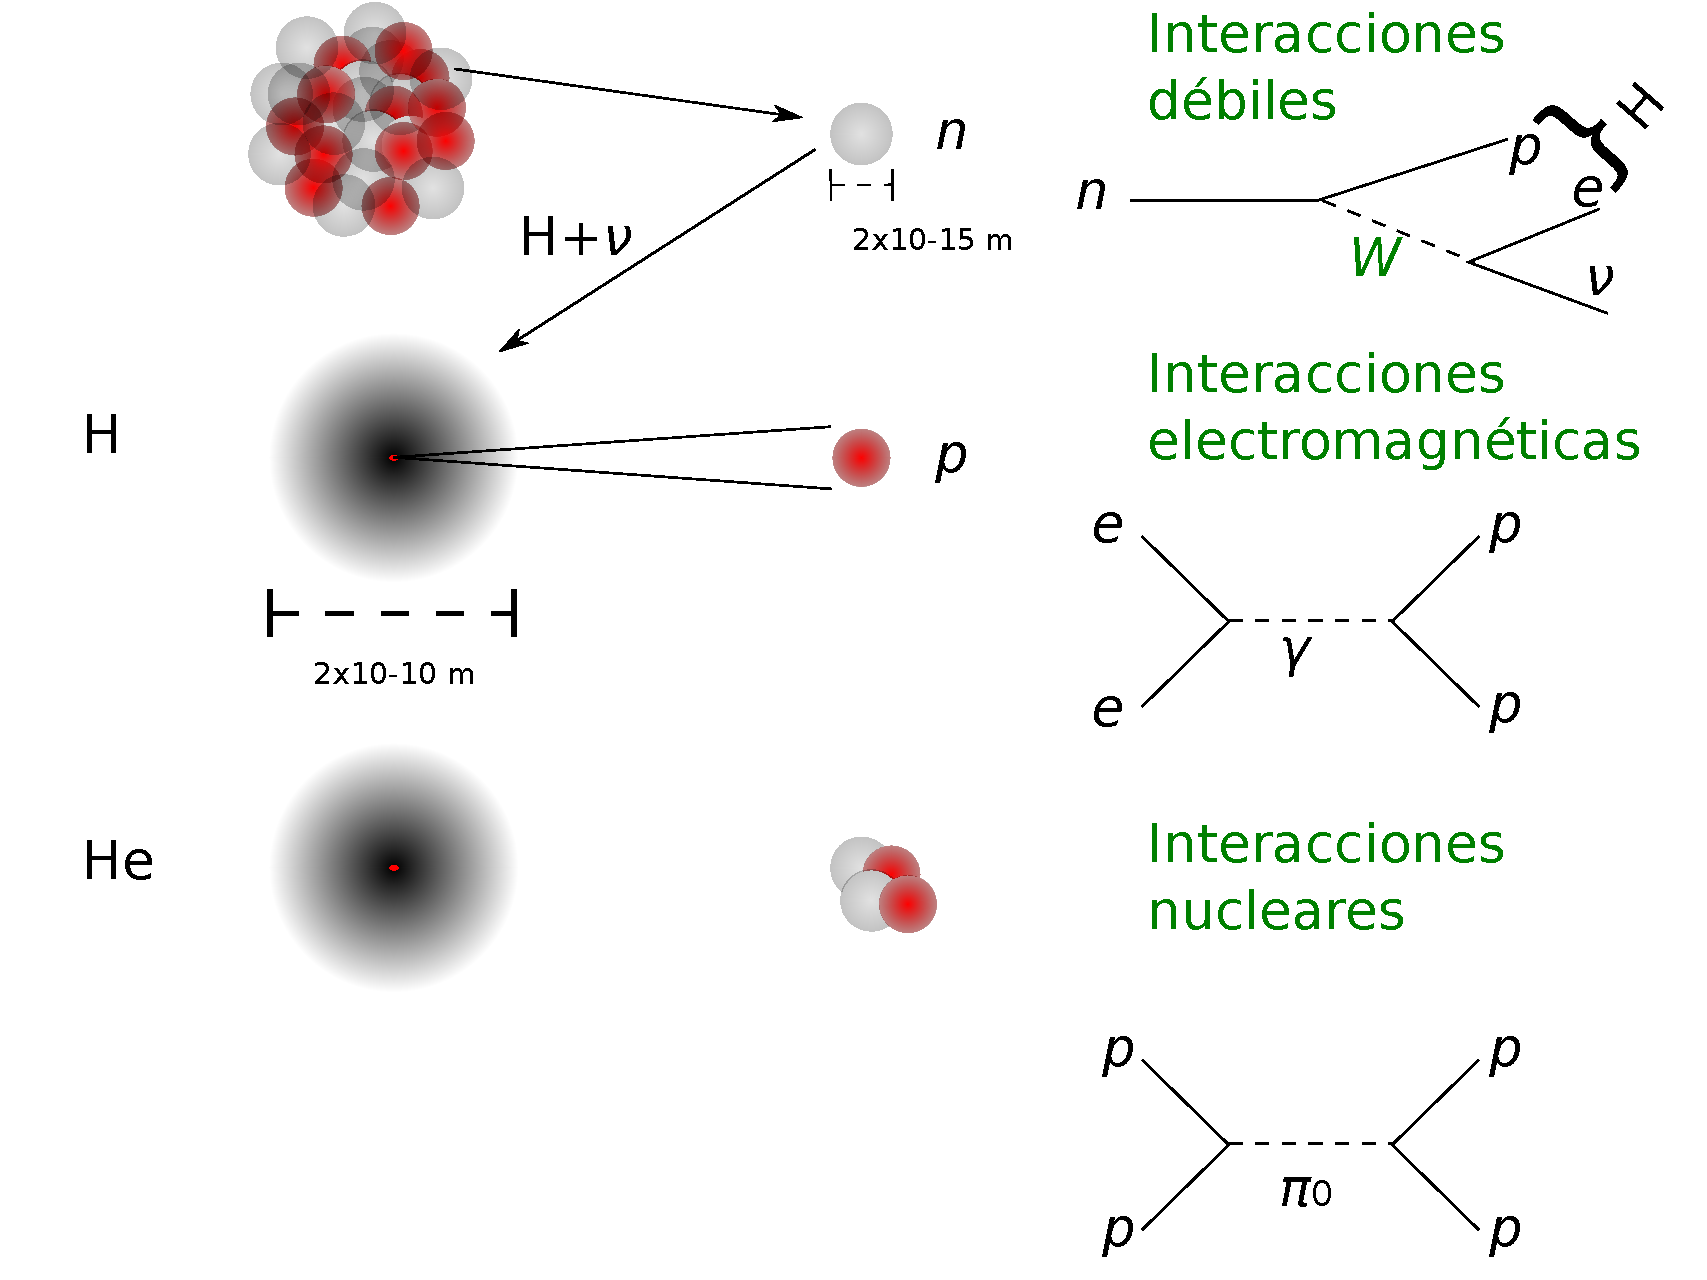
\includegraphics[width=\paperwidth]{interactions3}}
%\setbeamercovered{invisible}
\begin{frame}[plain]
\end{frame}
}
%%%%%%%%%%%%%%%%%%%%%%%%%%%%%%%%%%%%
{
\usebackgroundtemplate{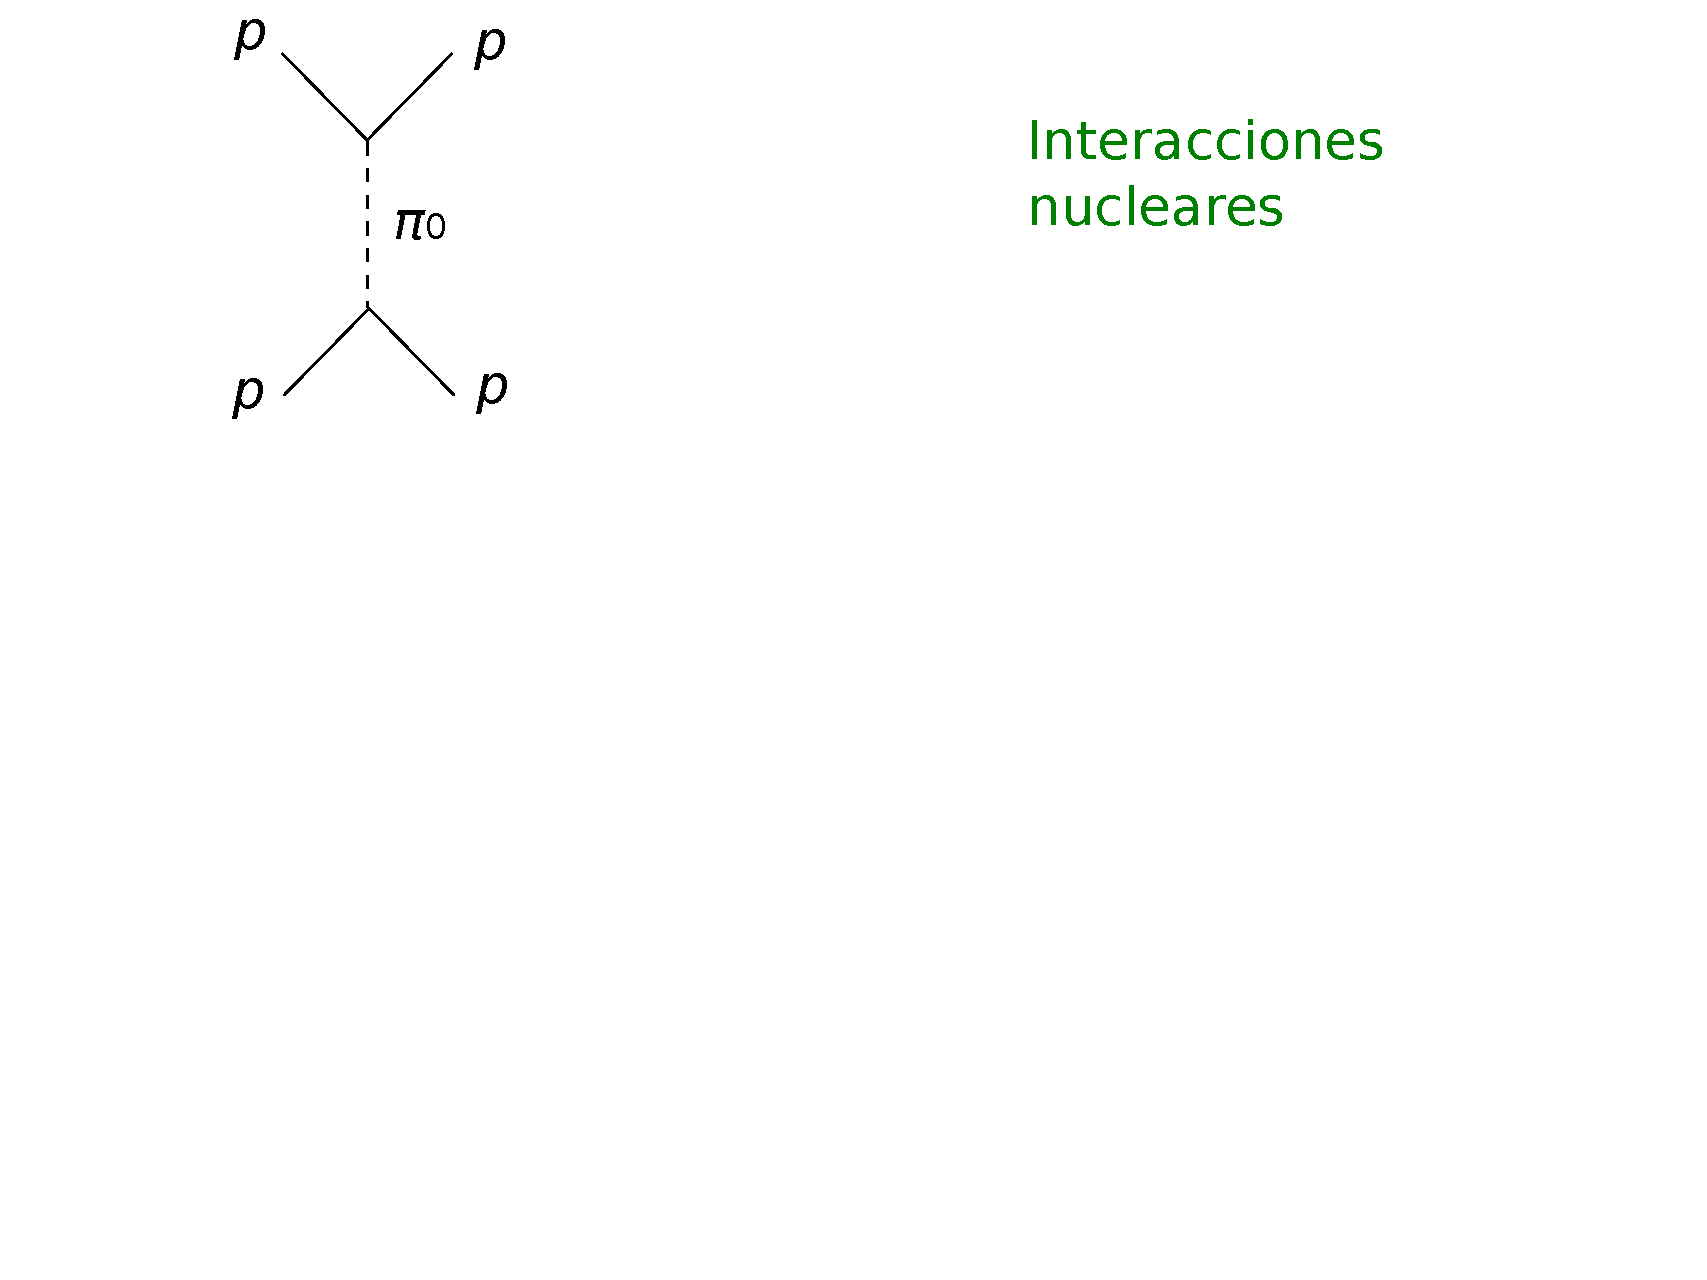
\includegraphics[width=\paperwidth]{interactions4a}}
%\setbeamercovered{invisible}
\begin{frame}[plain]
\end{frame}
}
%%%%%%%%%%%%%%%%%%%%%%%%%%%%%%%%%%%%
{
\usebackgroundtemplate{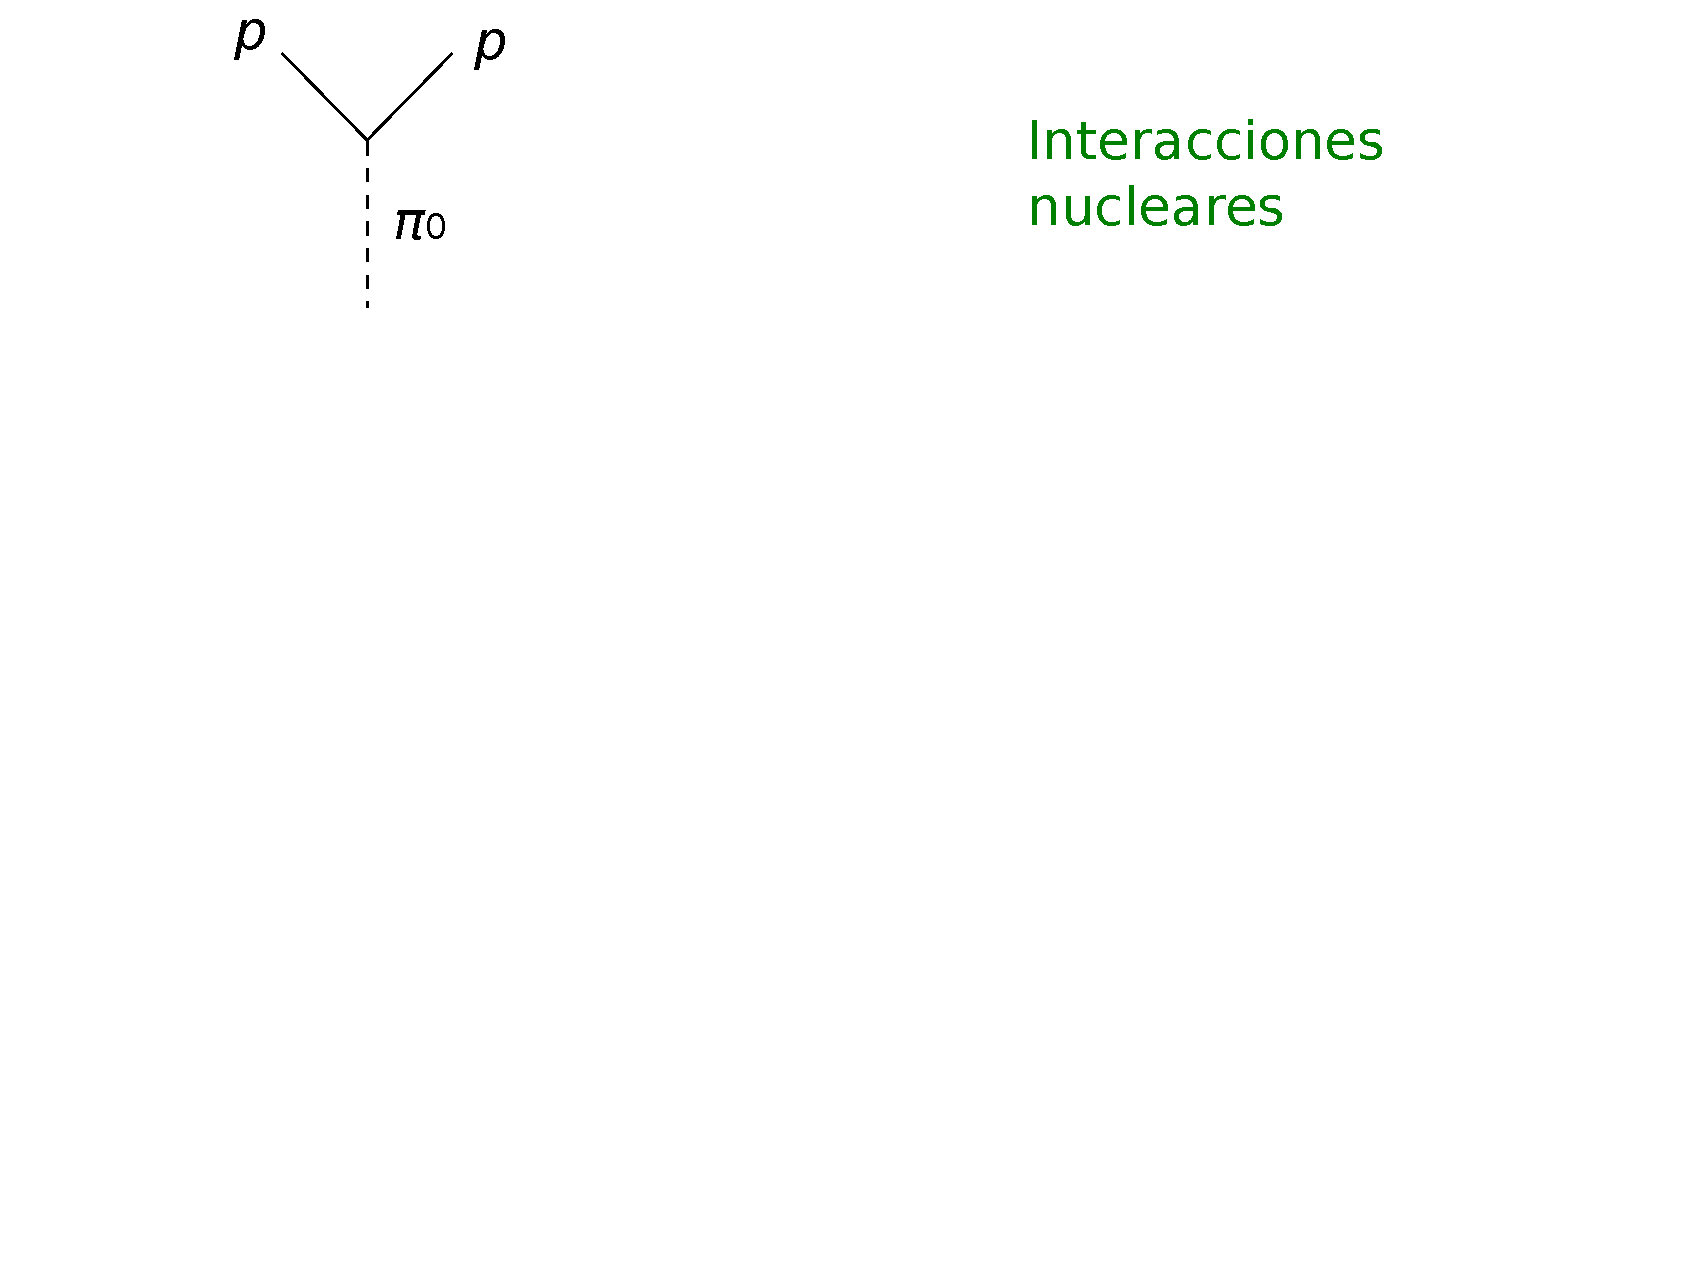
\includegraphics[width=\paperwidth]{interactions4b}}
%\setbeamercovered{invisible}
\begin{frame}[plain]
\end{frame}
}
%%%%%%%%%%%%%%%%%%%%%%%%%%%%%%%%%%%%
{
\usebackgroundtemplate{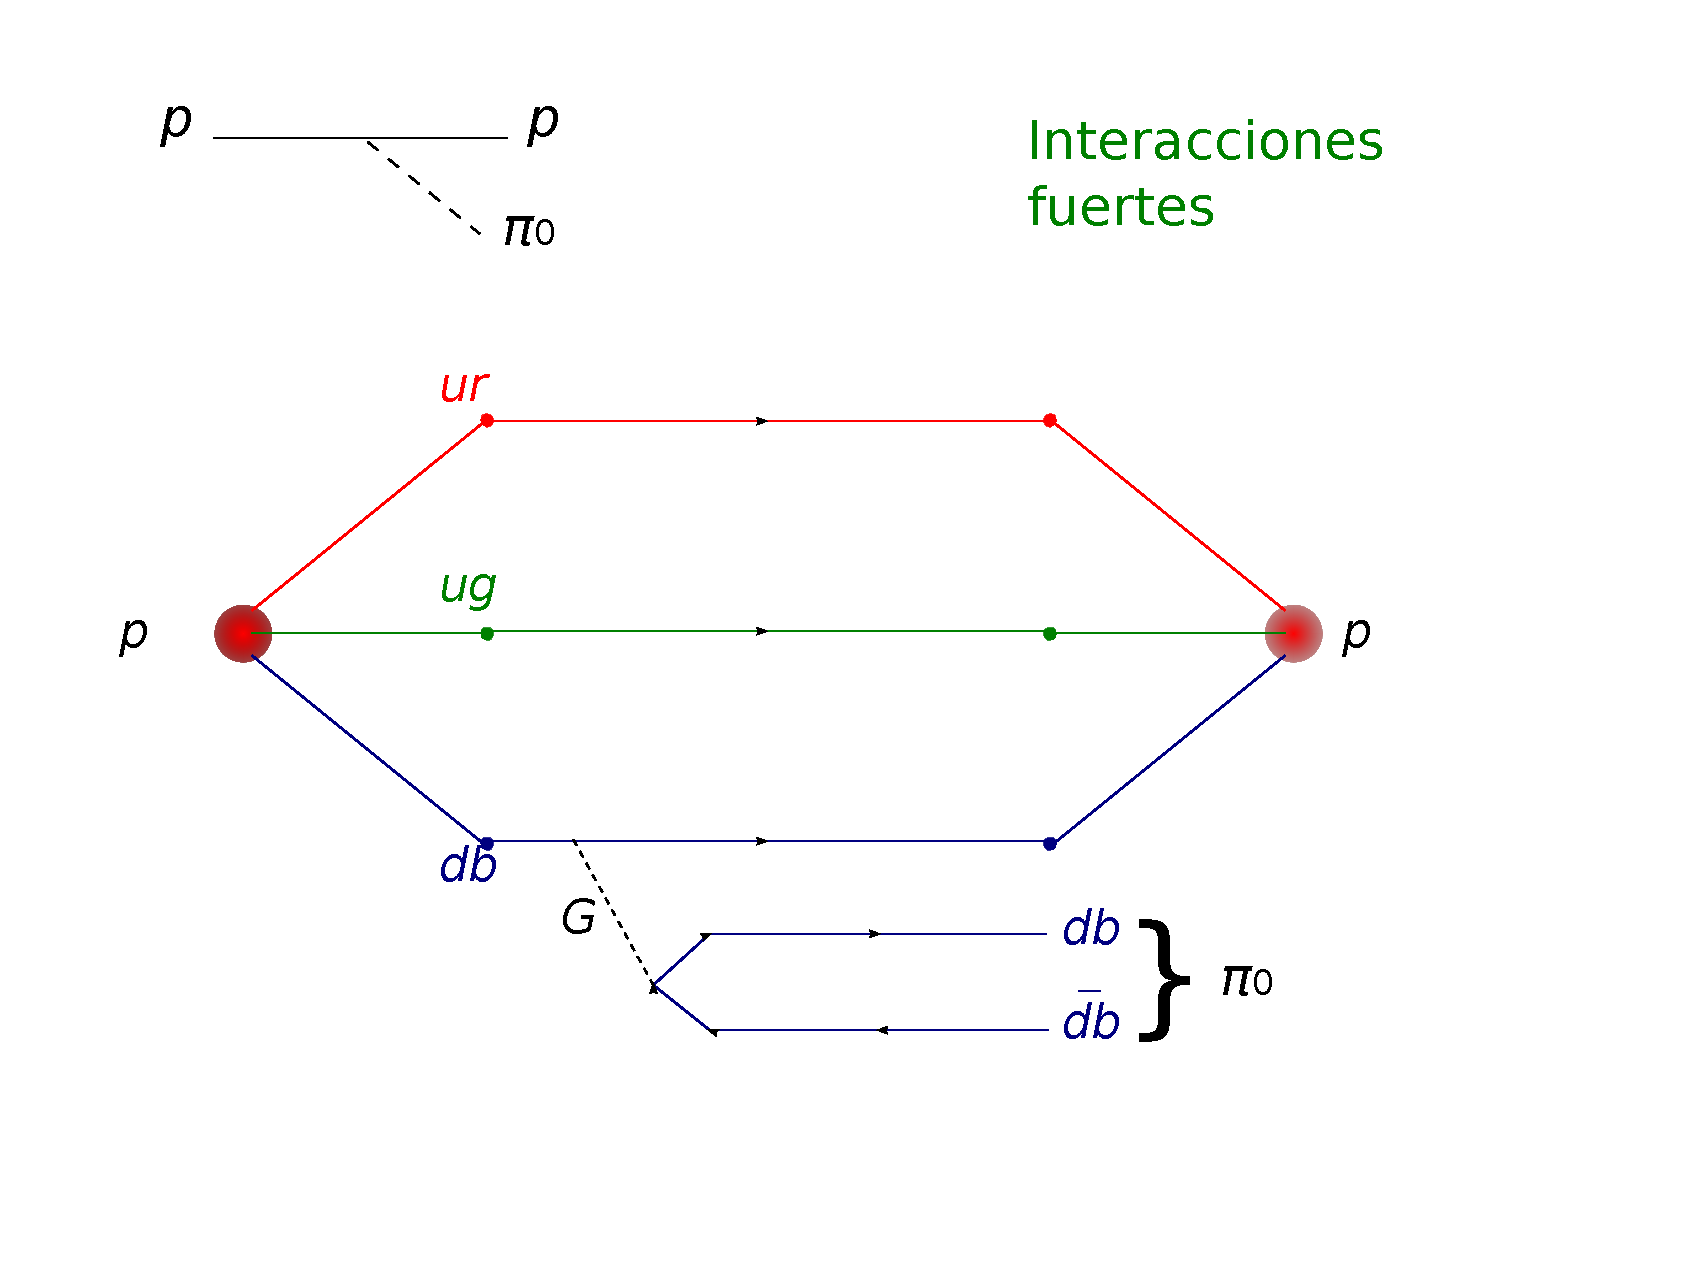
\includegraphics[width=\paperwidth]{interactions4c}}
%\setbeamercovered{invisible}
\begin{frame}[plain]
\end{frame}
}

\begin{frame}
    \begin{align*}
      \begin{pmatrix}
        \color{red}{r\bar{r}} & \color{red}{r}\bar{b} &\color{red}{r}\bar{g}\\ 
        \color{blue}{b}\color{red}{\bar{r}} & \color{blue}{b\bar{b}} &\color{blue}{b}\color{Green}{\bar{g}}\\ 
        \color{Green}{g}\color{red}{\bar{r}} & g\color{blue}{\bar{b}} &\color{Green}{g\bar{g}}\\ 
      \end{pmatrix},\qquad\text{with}\quad 
      \color{red}{r\bar{r}}+\color{blue}{b\bar{b}}+\color{Green}{g\bar{g}}=0
    \end{align*}
  \begin{columns}
    \begin{column}{0.5\textwidth}
    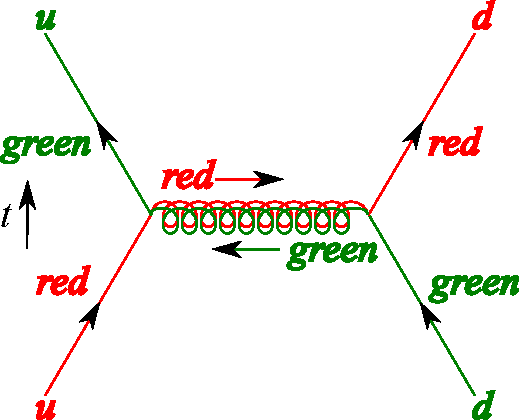
\includegraphics[scale=0.7]{qcd}      
    \end{column}
    \begin{column}{0.5\textwidth}
      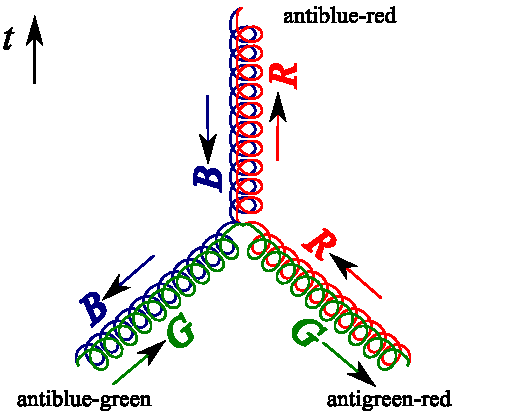
\includegraphics[scale=0.7]{qcd3gluon}      
    \end{column}
  \end{columns}
\end{frame}
\begin{frame}
  \frametitle{Conservación de la carga eléctrica}
  \only<1>{electrón} \hspace{0.8\textwidth} \only<2>{electrón}

  \only<3>{electrón}\only<4>{\hspace{1cm}$\overset{c}{\longrightarrow}$ electrón}
  
  \only<4>{\hspace{1.5cm}fotón sin masa}


\end{frame}


%%%%%%%%
{
\usebackgroundtemplate{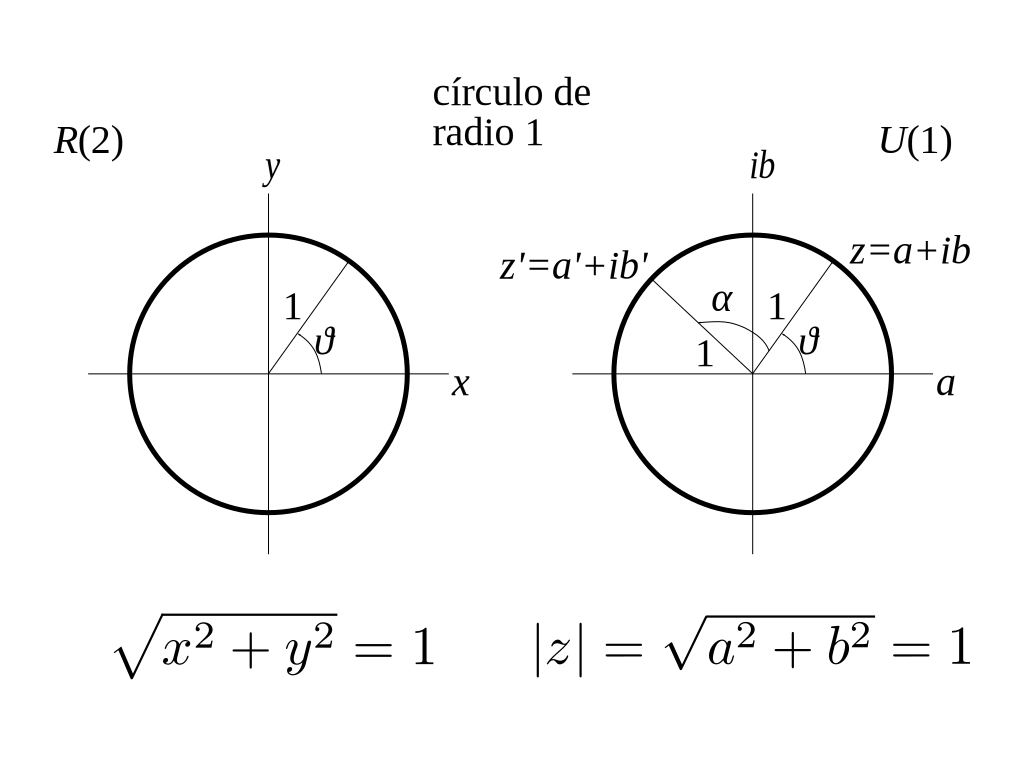
\includegraphics[width=\paperwidth]{r2u1}}
%\setbeamercovered{invisible}
\begin{frame}[plain]
  \begin{block}{Números complejos}
  Números imaginarios: $i^2=-1$; $(ib)^2=-b$\\
  Número complejo: $z=a+ib$, con $a$ y $b$ reales\\
  \begin{equation*}
  |z|=\sqrt{a^2+b^2}  
  \end{equation*}
  Fórmula de euler: $z=|z|e^{i\theta}=|z|(cos\theta+i\sin\theta)$
  \begin{align*}
    a=&|z|cos\theta&b=&|z|\sin\theta
  \end{align*}
  Cambio de fase: $z\to z'=|z|e^{i(\theta+\alpha)}=e^{i\alpha}|z|e^{i\theta}=e^{i\alpha}z$
  \begin{align*}
    \text{t.q:}\quad|z'|=|z|
  \end{align*}

\vspace{2cm}
\quad
  \end{block}
\end{frame}
}

%%%%%%%%
{
\usebackgroundtemplate{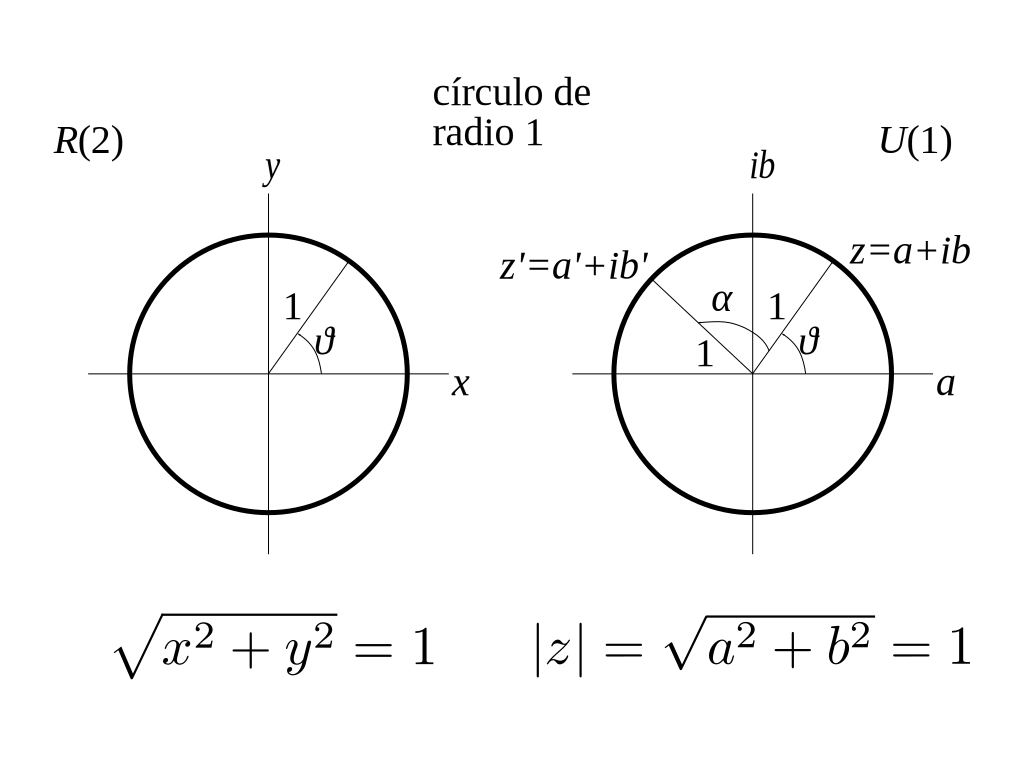
\includegraphics[width=\paperwidth]{r2u1}}
%\setbeamercovered{invisible}
\begin{frame}[plain]
\end{frame}
}
%%%%%%%%
{
\usebackgroundtemplate{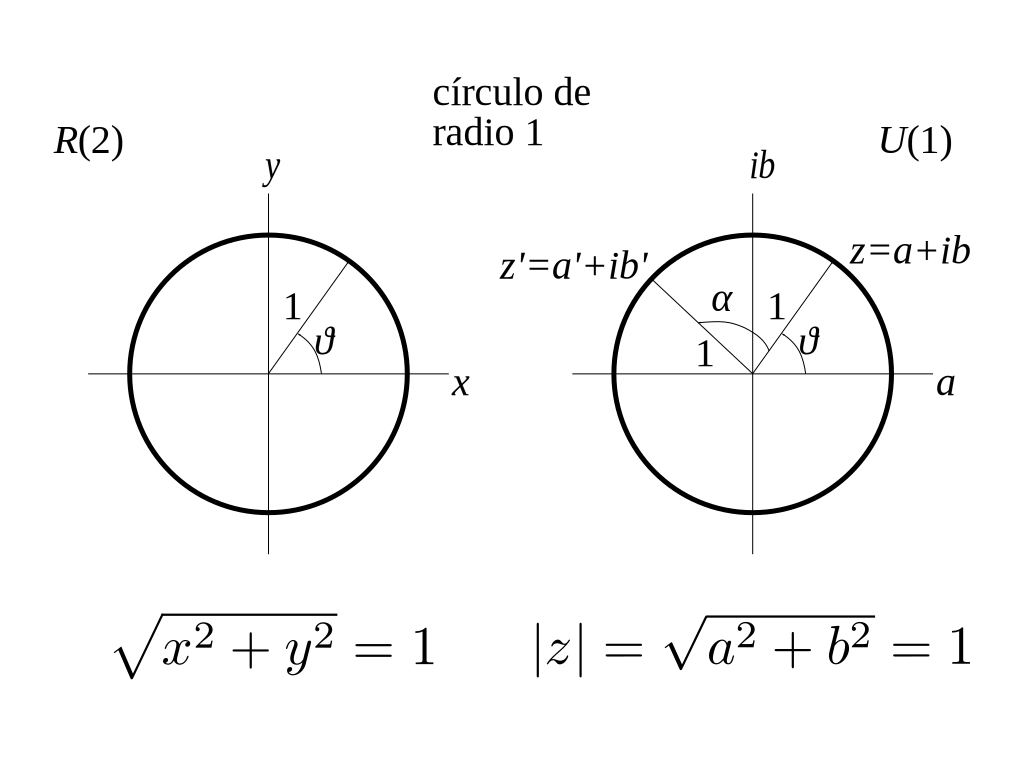
\includegraphics[width=\paperwidth]{r2u1}}
%\setbeamercovered{invisible}
\begin{frame}[plain]
  \begin{block}{La función de onda}
    La escogencia de la fase de la función de onda es arbitraria:    
    \begin{equation*}
      -\frac{h^2}{8\pi^2m}\frac{d^2}{dx^2}\psi(x)=E\psi(x)
    \end{equation*}
    \begin{equation*}
      \left|\psi(x)\right|^2=1
    \end{equation*}
Invarianza bajo $U(1)$, $\alpha=$constante: 
\begin{align*}
  \psi(x)\to e^{i\alpha}\psi(x)
\end{align*}
La cantidad conservada es la probabilidad.
\begin{align*}
  \psi(x)=\text{probabilidad}\times\exp{(i x\cdot p)}
\end{align*}
y para $x=(t,\mathbf{x})$ homogéneo:\\ 
$\Longrightarrow$ La energía y el momentum en mecánica cuántica

  \end{block}

\end{frame}
}
%%%%%%%%
%%%%%%%%
{
\usebackgroundtemplate{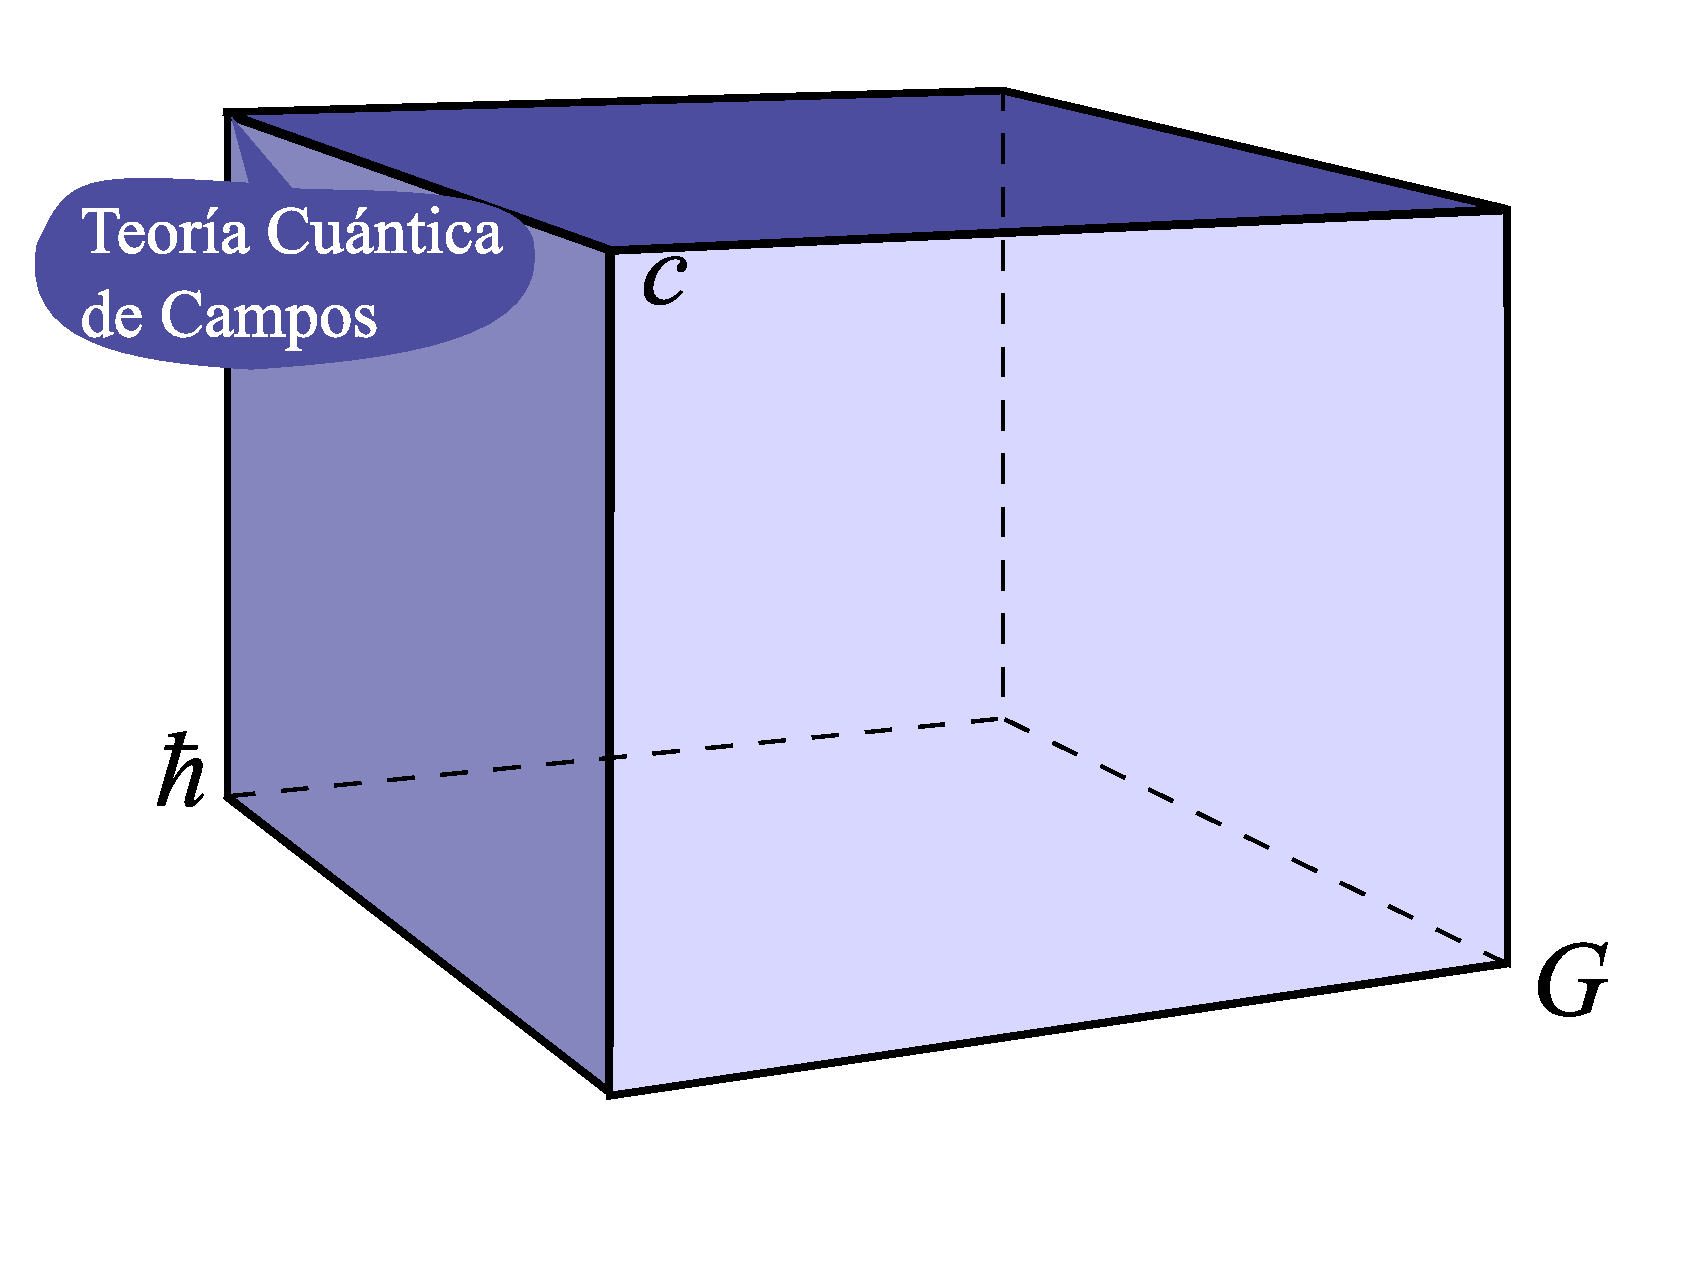
\includegraphics[width=\paperwidth]{gp-qft2}}
%\setbeamercovered{invisible}
\begin{frame}[plain]
\end{frame}
}
%%%%%%%%

{
\usebackgroundtemplate{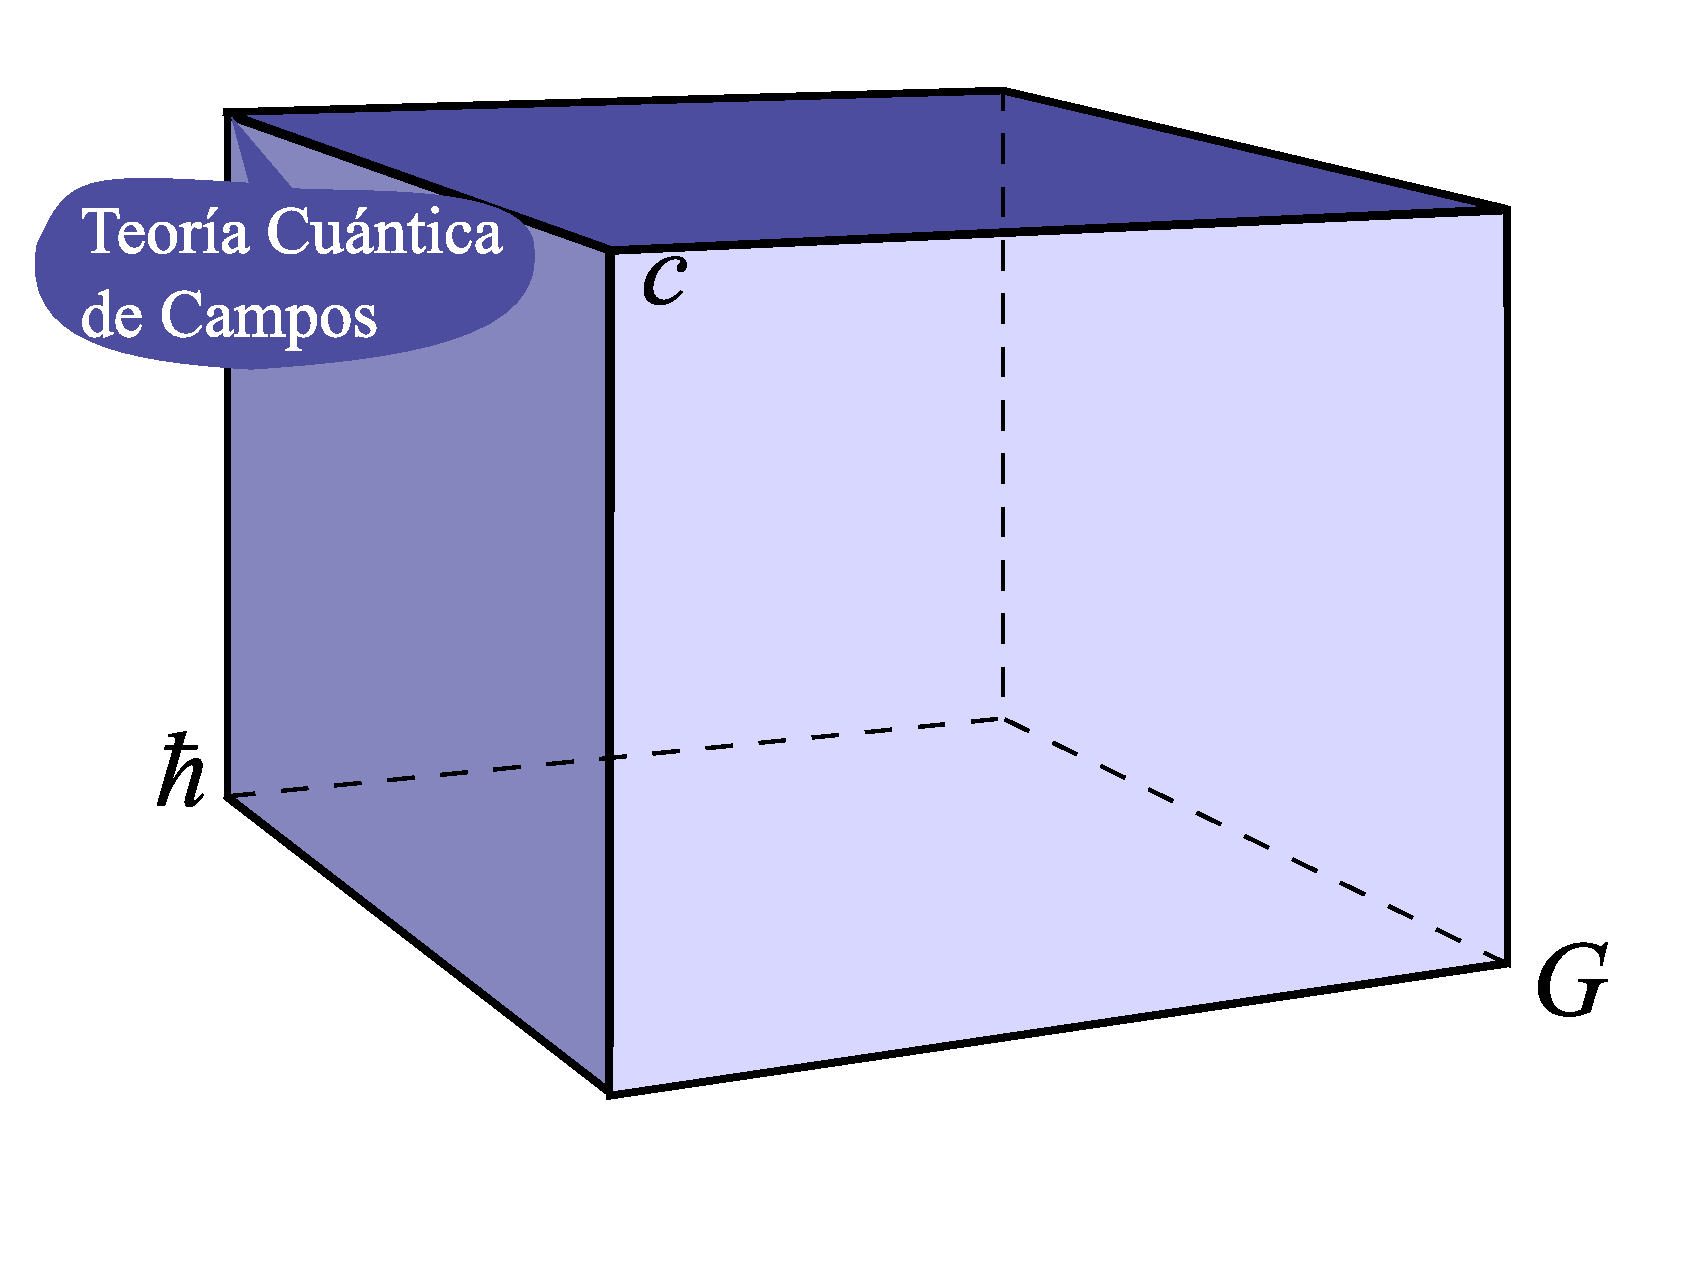
\includegraphics[width=\paperwidth]{gp-qft2}}
\begin{frame}[plain]


\begin{block}{}
  \begin{quote}
    Como se concibe usualmente, sin embargo, esta arbitrariedad esta sujeta a las siguientes limitaciones: una vez se escoge [la fase de la función de onda] en un punto del espacio tiempo, entonces ya no se tiene la libertad de hacer alguna escogencia en otros puntos del espacio-tiempo.

Parece ser que esto no es consistente con el concepto de campo localizado que subyace a las teorías física usuales. En el presente artículo deseamos explorar la posibilidad de requerir que todas las interacciones sean invariantes bajo [cambios de fase] independientes en todos los puntos del espacio tiempo
  \end{quote}
  \begin{flushright}
    Yang-Mills, \emph{Physical Review}, 1954
  \end{flushright}
\end{block}
\end{frame}
}
%%%%
%%%%%%%%
%\setbeamercovered{invisible}
\begin{frame}[plain]
  \begin{block}{Cambios locales en la función de onda: $\psi(x)\to e^{\alpha(x)}\psi(x)$}
    \begin{equation*}
      -\frac{h^2}{8\pi^2m}\frac{d^2}{dx^2}\psi(x)=E\psi(x)
    \end{equation*}
Cada vez que la función de onda cambia localmente, el resultado de la operación derivada cambia, introduciendo algún error que causa que la función de onda no siga satisfaciendo la ecuación de onda.

Yang y Mills entonces propusieron una trampa: adicionar un nuevo término que cancelara el efecto de la operación de rata de cambio:
\begin{equation*}
  q A(x)\psi(x)
\end{equation*}

Cualquier daño que el término de rata de cambio en la ecuación de onda cause cuando la fase de la función de onda es cambiada localmente, $A(x)$ debe ser lo que sea para reparar el daño.

El efecto neto es que la ecuación de onda cambia, y la nueva ecuación debe estar describiendo una situación física diferente a la de la función de onda original.

El cambio requerido en $A(x)$ es justo el tipo de cambio que deja el campo electromagnético invariante.
  \end{block}
\end{frame}
%%%%%%%%
\begin{frame}[allowframebreaks]
  \frametitle{QED}
  \begin{itemize}
  \item   La nueva situación física que surge de la nueva ecuación de onda que es invariante bajo cambios locales de fase es la que combina satisfactoriamente la mecánica cuántica con el electromagnetismo:

  \item Para compensar los cambios locales de fase, debemos cambiar $A(x)$ en una forma particular, dependiendo en como se cambio la fase a través del espacio tiempo. Los cambios en $A(x)$ no tienen significado físico.

  \item El requerimiento de que la función de onda sea invariante bajo cambios locales de fase ha necesitado la introducción del electromagnetismo.

  \end{itemize}
\end{frame}


%%%%%%%%
{
\usebackgroundtemplate{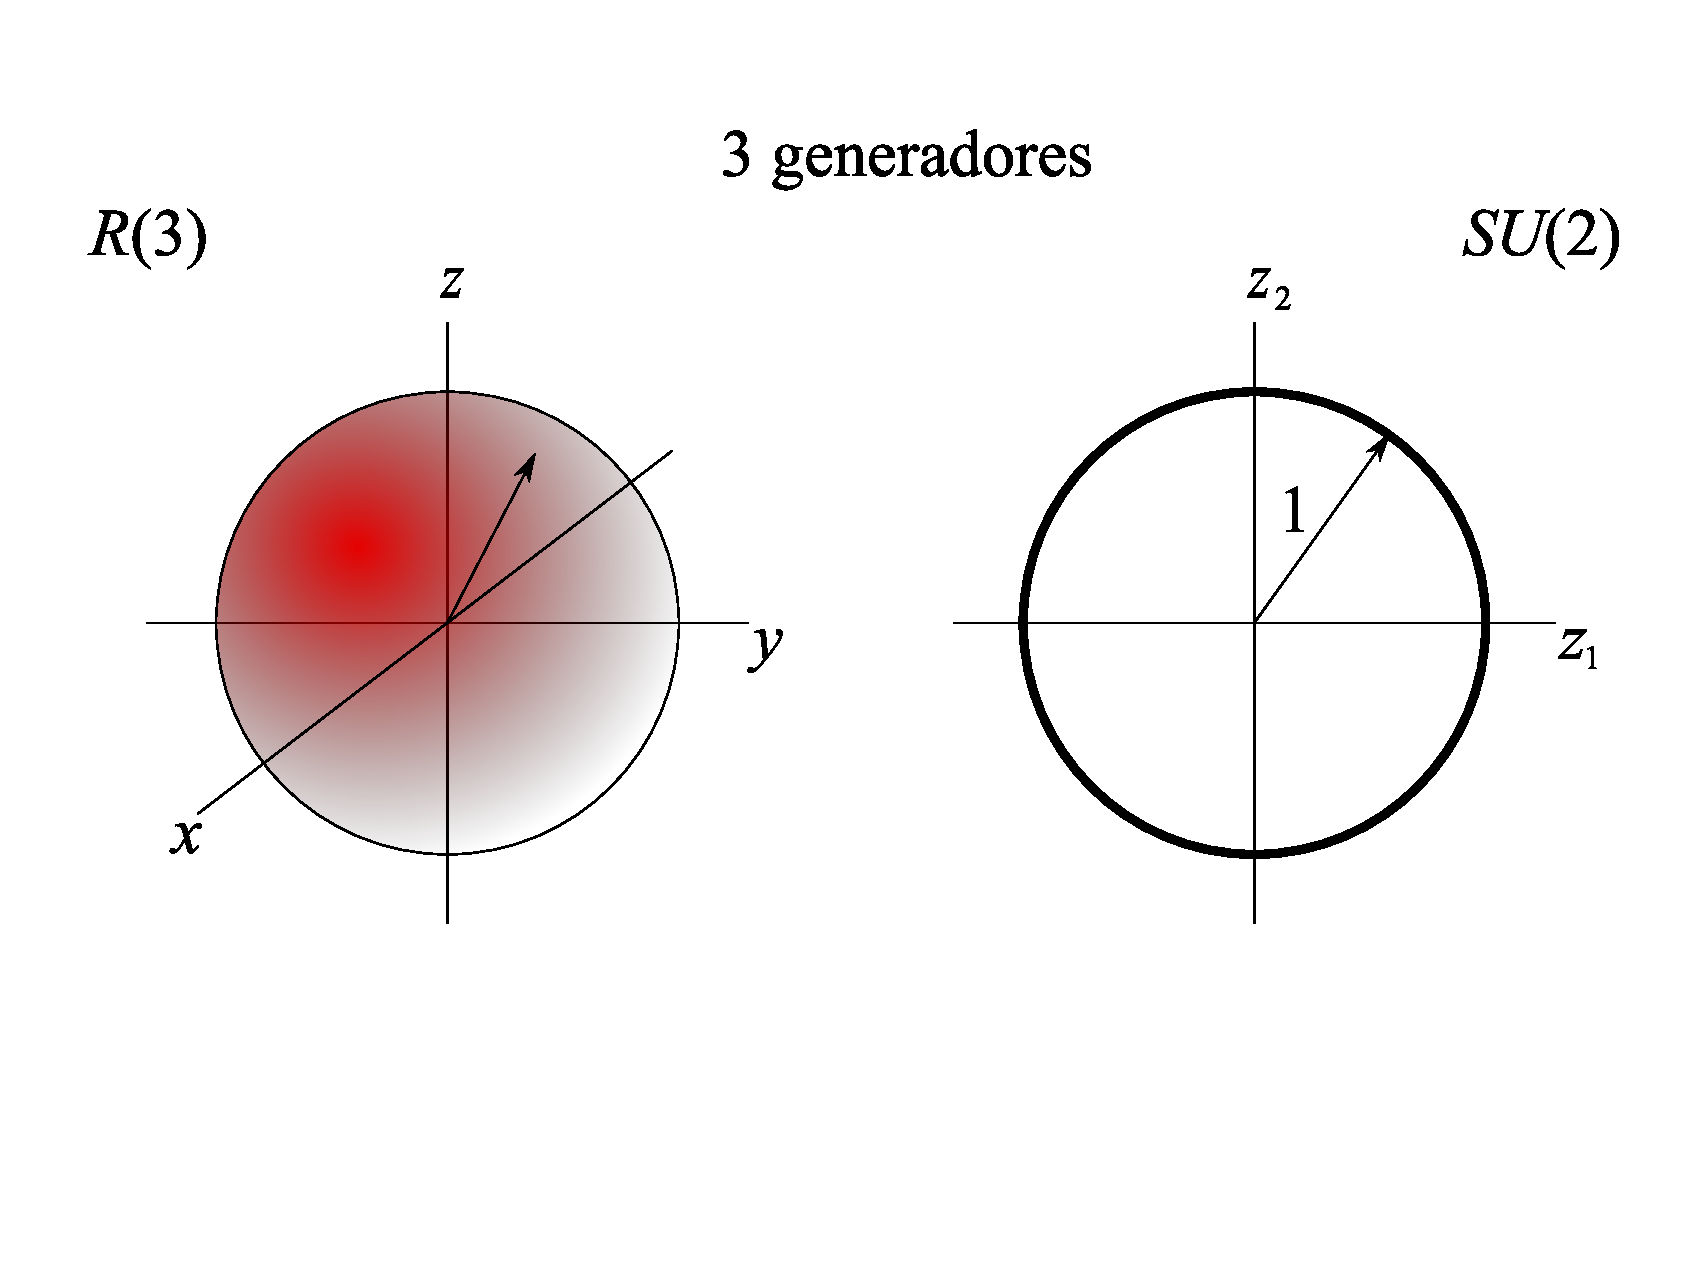
\includegraphics[width=\paperwidth]{r3su2}}
%\setbeamercovered{invisible}
\begin{frame}[plain]
\end{frame}
}

%%%%%%%%
{
\usebackgroundtemplate{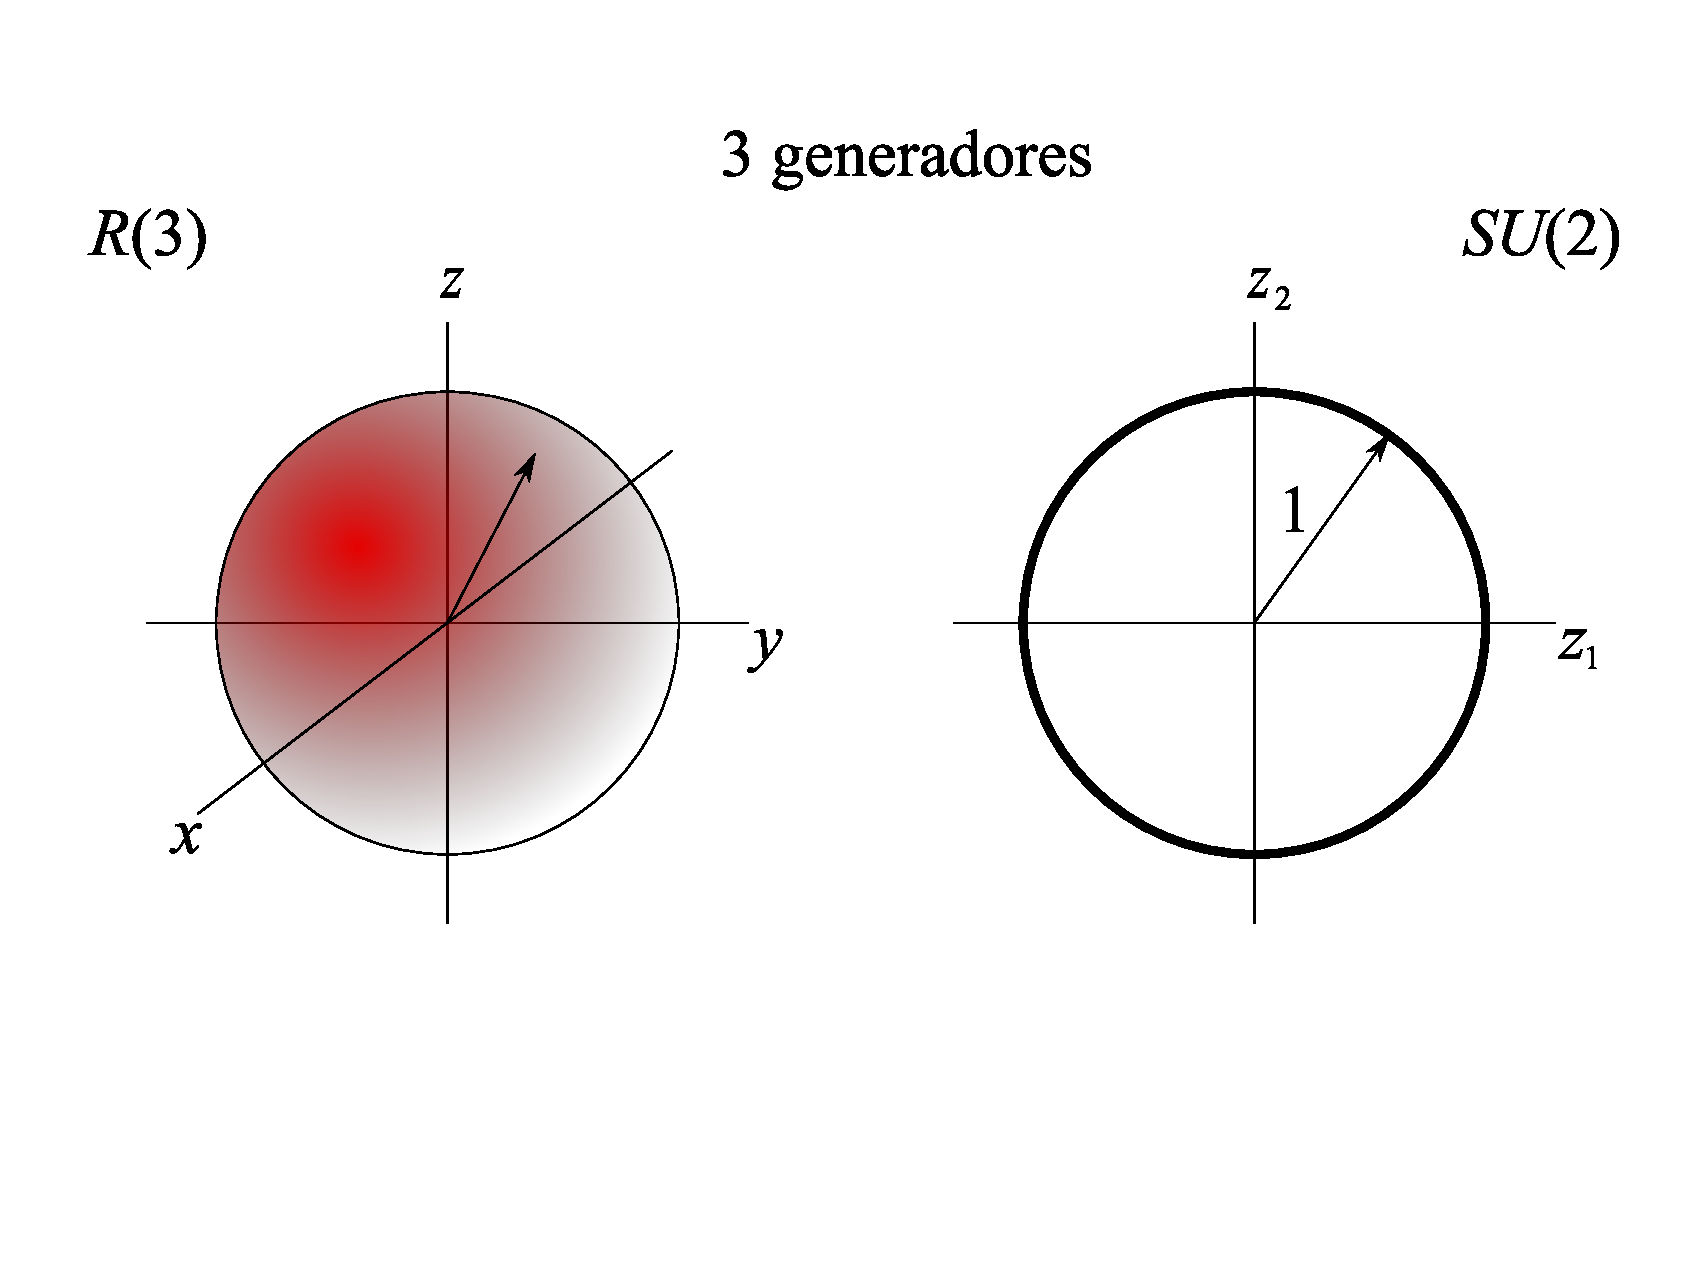
\includegraphics[width=\paperwidth]{r3su2}}
\setbeamercovered{invisible}
\begin{frame}[plain]
  \begin{block}<1->{Isospin fuerte}
    \begin{align*}
      p&\to \psi_1(x)\\
      n&\to \psi_2(x)\\
    \end{align*}
  \end{block}
  \begin{block}<2->{Isospin débil}
    \begin{align*}
      \nu&\to \psi_1(x)\\
      e&\to \psi_2(x)\\
    \end{align*}
  \end{block}

\end{frame}
}

\begin{frame}
  \frametitle{$SU(3)$}
  Considere el quark up: $u$
  \begin{align*}
   \color{red} u_1=u_{\text red}&\to \psi_1(x)\\
    \color{Green}u_2=u_{\text green}&\to \psi_2(x)\\
    \color{blue}u_1=u_{\text blue}&\to \psi_3(x)
  \end{align*}

\end{frame}




%%%%%%%%%%%%%%%%%%
\begin{frame}
  \frametitle{Conservación del isospín débil}
\centering

  \only<1-2>{electrón\phantom{(L)}$\longleftrightarrow$ neutrino}\only<3->{electrón(L)$\longleftrightarrow$ neutrino}


  \only<1>{\phantom{electrón sin masa}}\only<2->{\hspace{1.5cm}\alert{electrón sin masa}}



  \only<4->{quark u(L) $\longleftrightarrow$ quark d(L)}

\only<4->{\hspace{1.5cm}\alert{quark sin masa}}

\end{frame}
\begin{frame}[plain]
\begin{picture}(320,250)
\only<1->{\put(-10,70){
\includegraphics[width=1.05\paperwidth]{what-is-real}}}%
\only<1->{\put(130,220){
    \begin{minipage}[t]{0.6\linewidth}
      ¿Es la masa algo real? 

     ¿O es simplemente el resultado de algunas\par interacciones?

     ¿Es posible distinguir entre ambas\par situaciones?
    \end{minipage}
}}
\only<2>{
\put(0,76.9){  \begin{minipage}[t]{1\linewidth}
    \begin{block}{Respuesta}
    Hasta ahora toda la masa parece ser pura apariencia
  \end{block}
  \end{minipage}
}
}
\end{picture}
\end{frame}

%%%%%%%%%%%%%%%%%%%%%%%%%%%%%%%%%%%%%%%%%%%%%%%%%%%%%%%
%Niveles de energia
%%%%%%%%%%%%%%%%%%%%%%%%%%%%%%%%%%%%
{
\usebackgroundtemplate{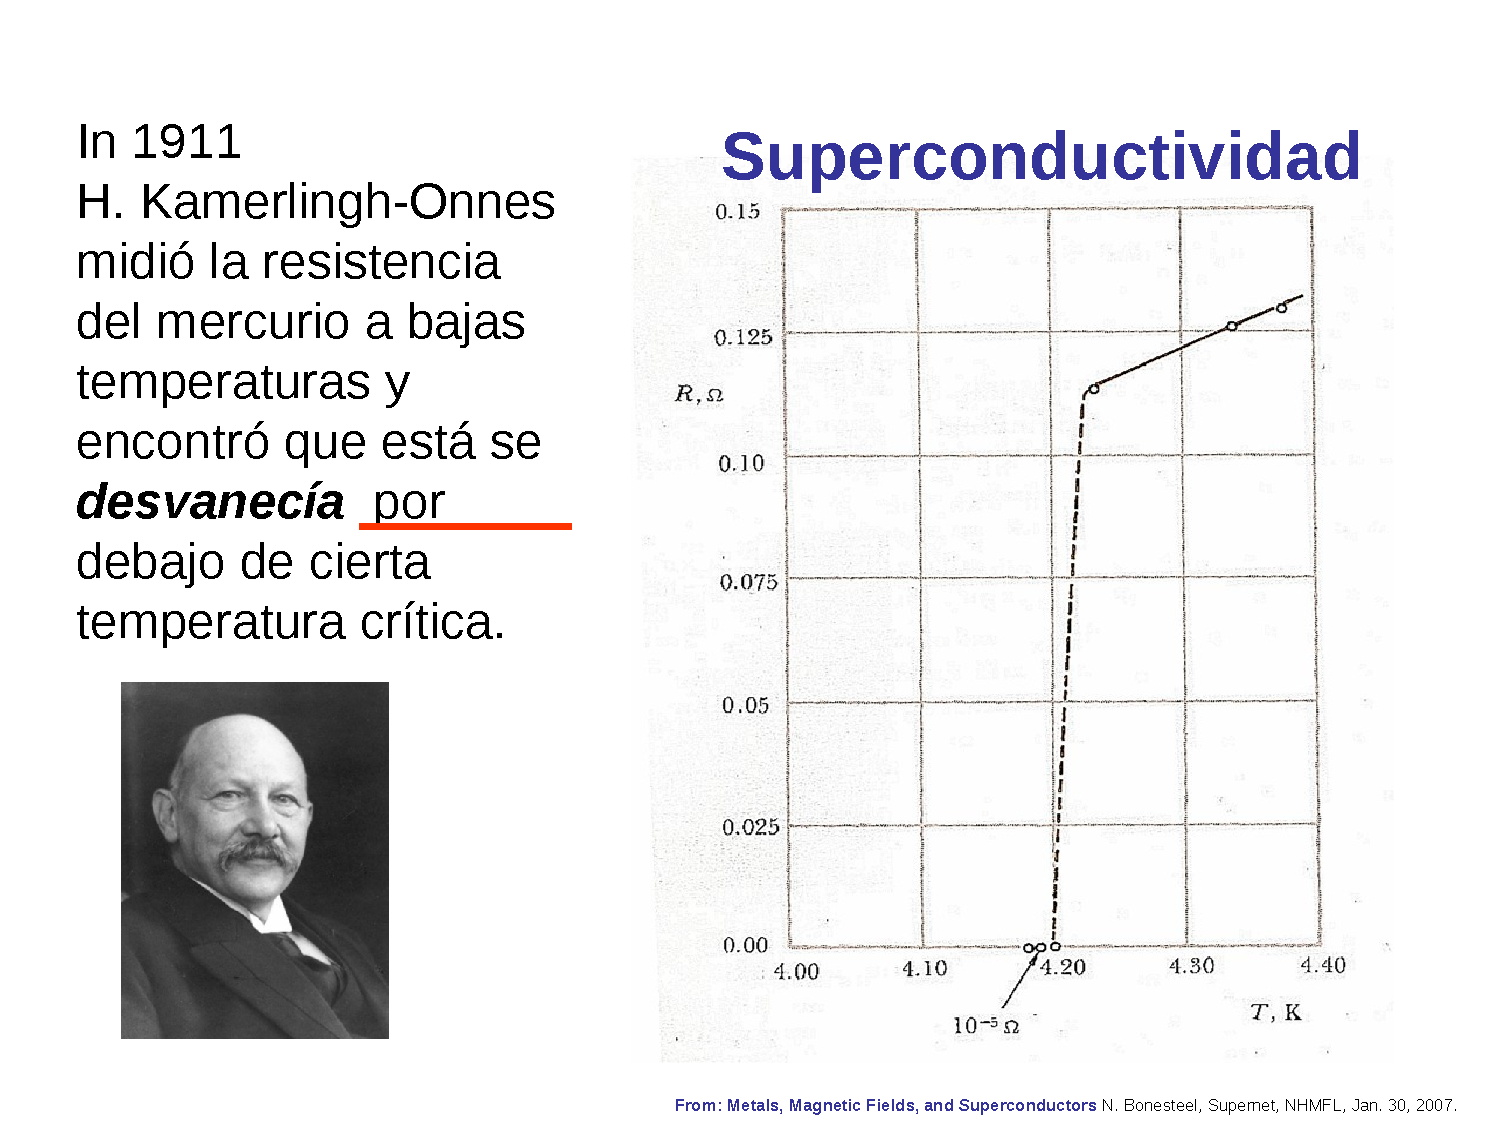
\includegraphics[width=\paperwidth]{superconductividad}}
%\setbeamercovered{invisible}
\begin{frame}{Resurgimiento del éter}

\end{frame}
}
%%%%%%%%
{
\usebackgroundtemplate{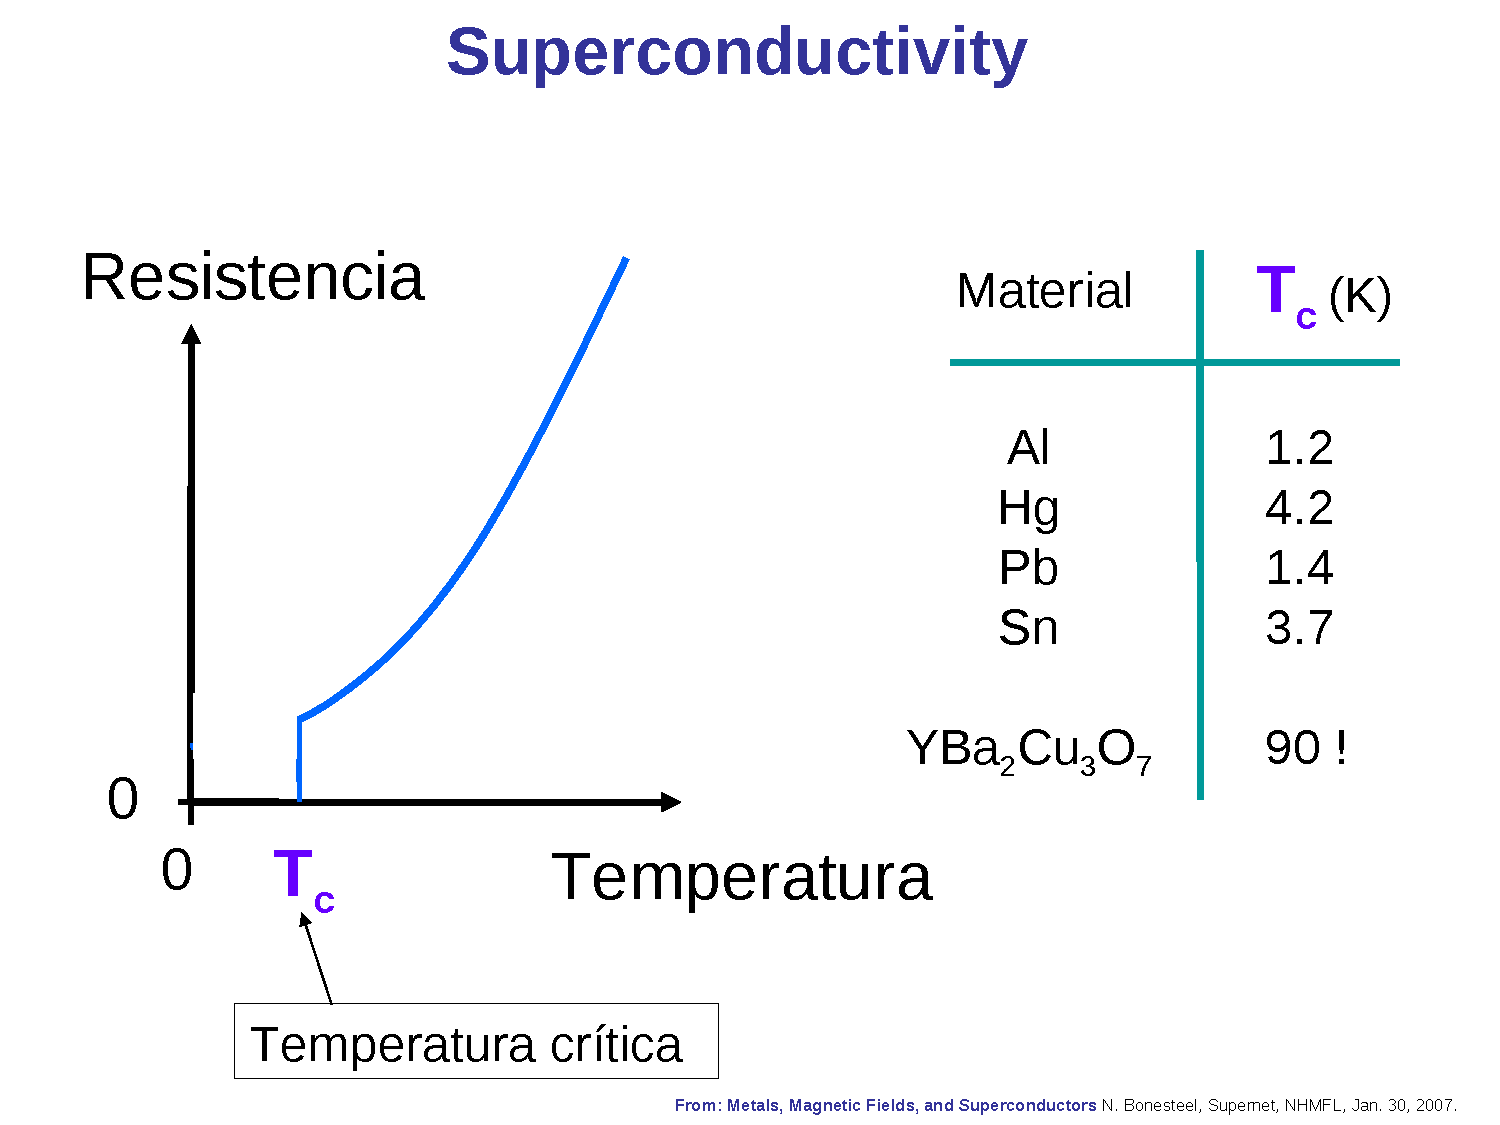
\includegraphics[width=\paperwidth]{resistencia}}
%\setbeamercovered{invisible}
\begin{frame}[plain]
\end{frame}
}
%%%%%%%%
{
\usebackgroundtemplate{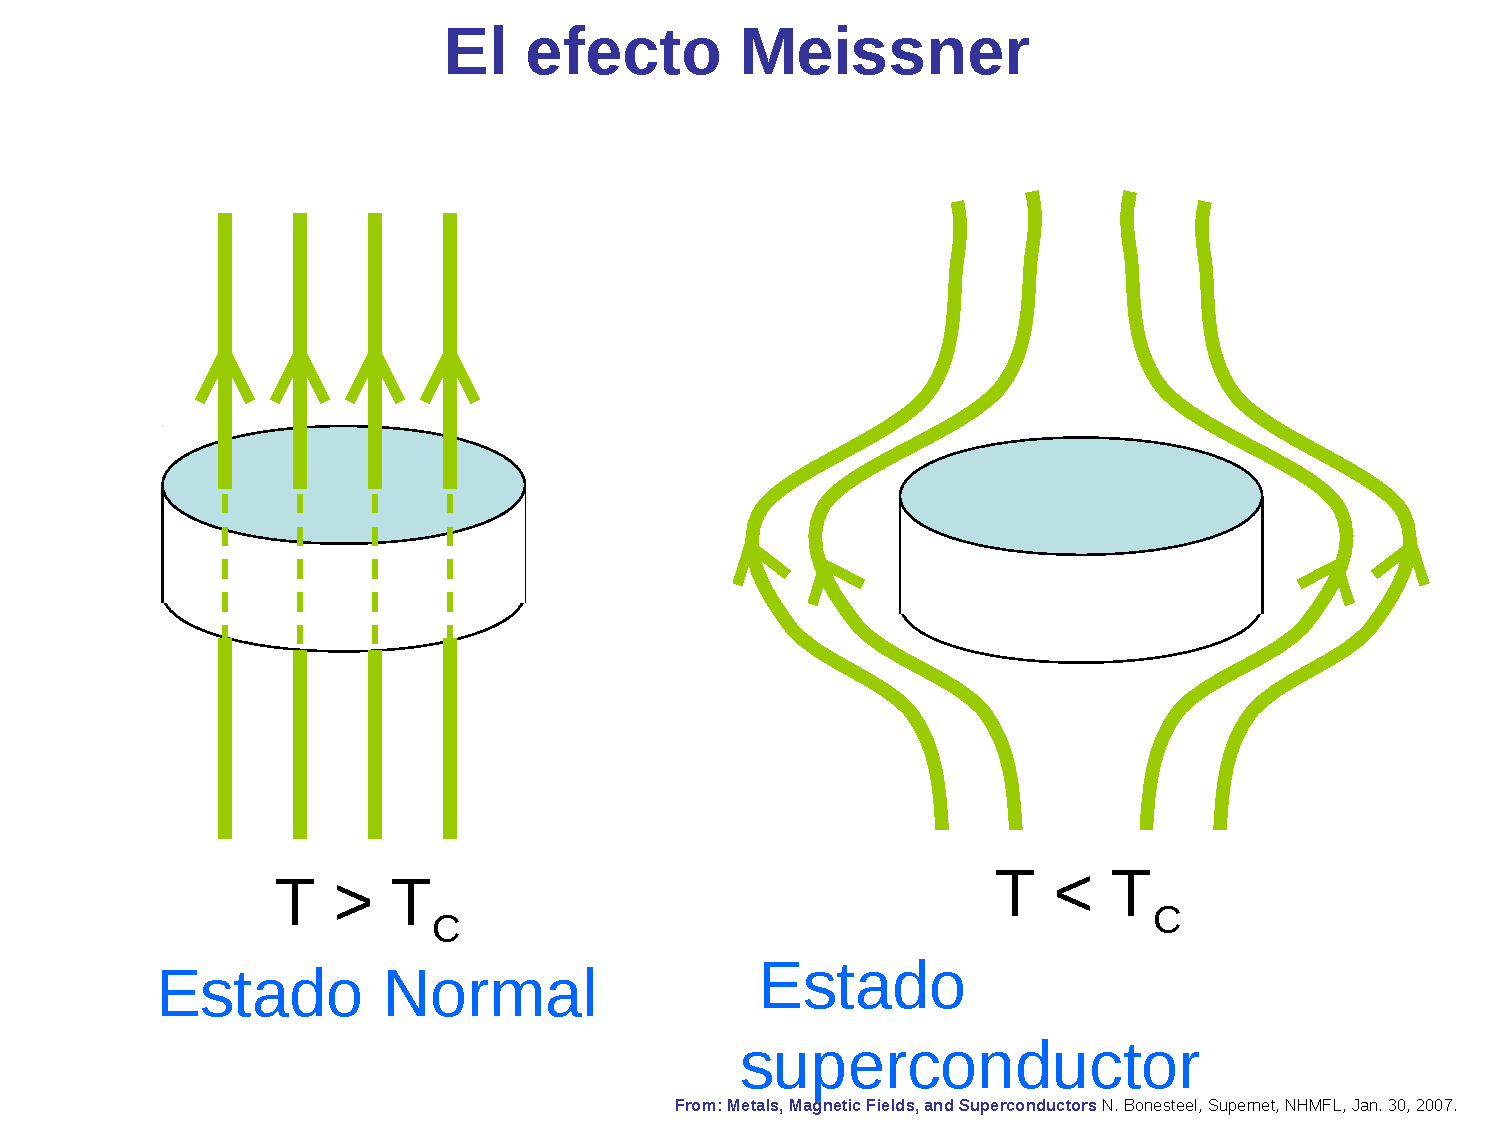
\includegraphics[width=\paperwidth]{meissner}}
%\setbeamercovered{invisible}
\begin{frame}[plain]
\end{frame}
}
%%%%%%%%
%%%%%%%%
{
\usebackgroundtemplate{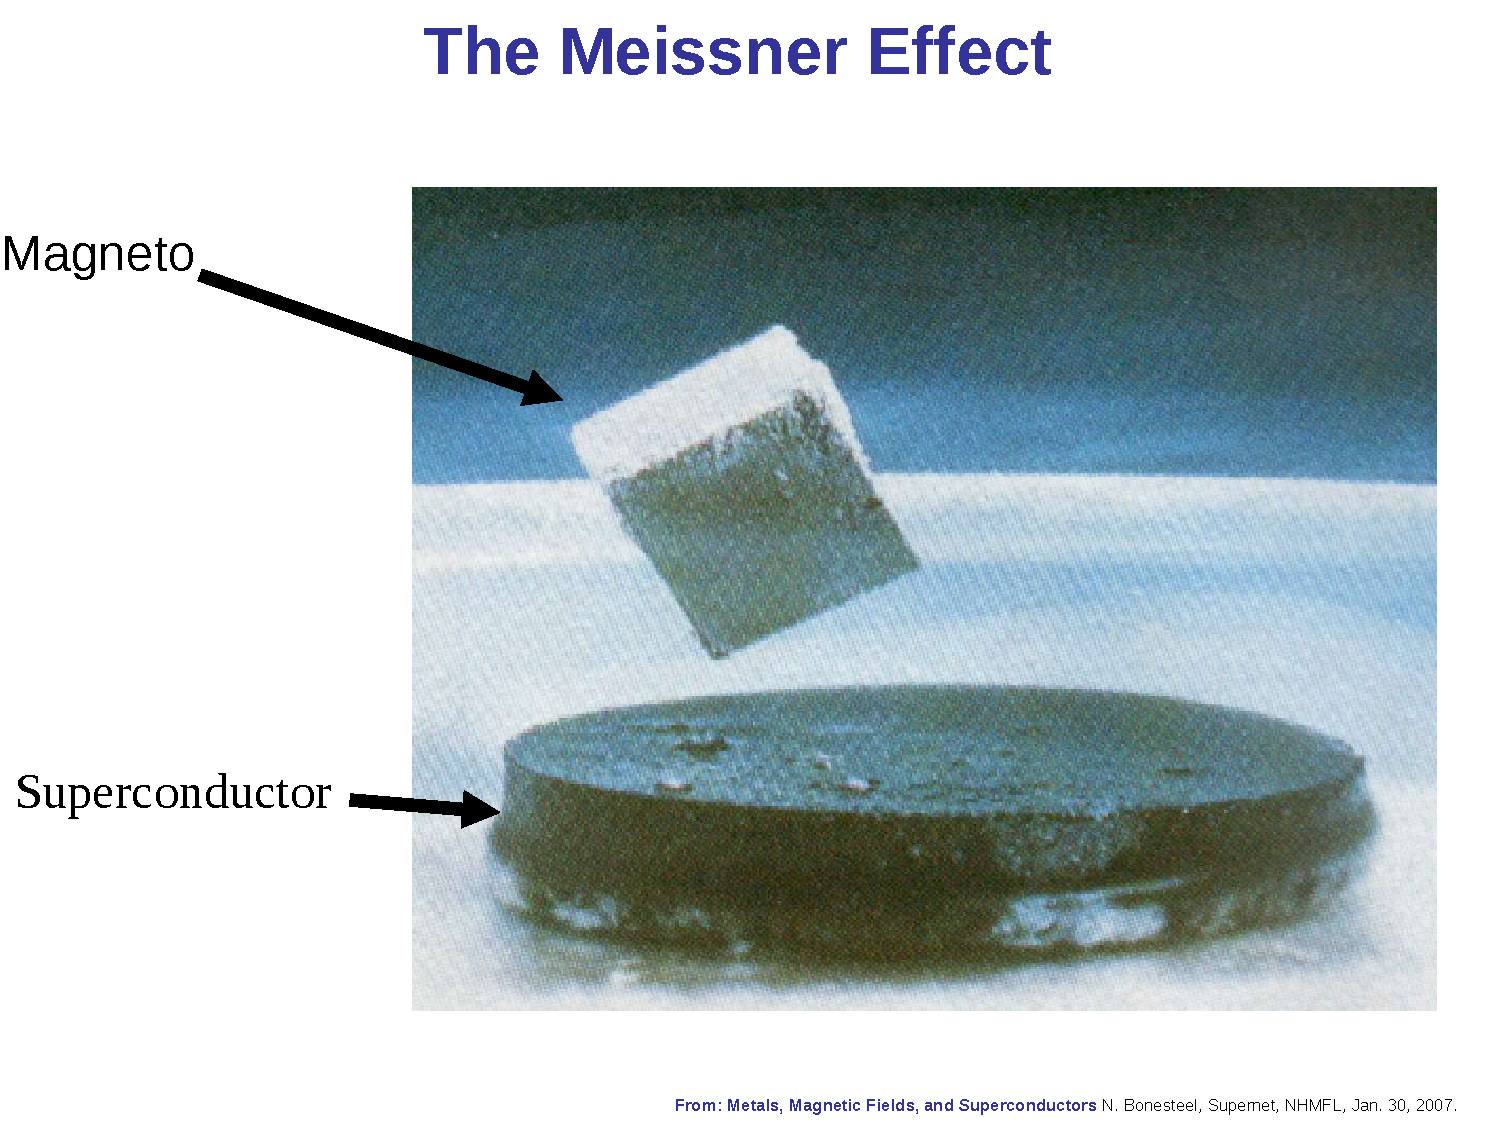
\includegraphics[width=\paperwidth]{meissner2}}
%\setbeamercovered{invisible}
\begin{frame}[plain]
\end{frame}
}
%%%%%%%%
%%%%%%%%
{
\usebackgroundtemplate{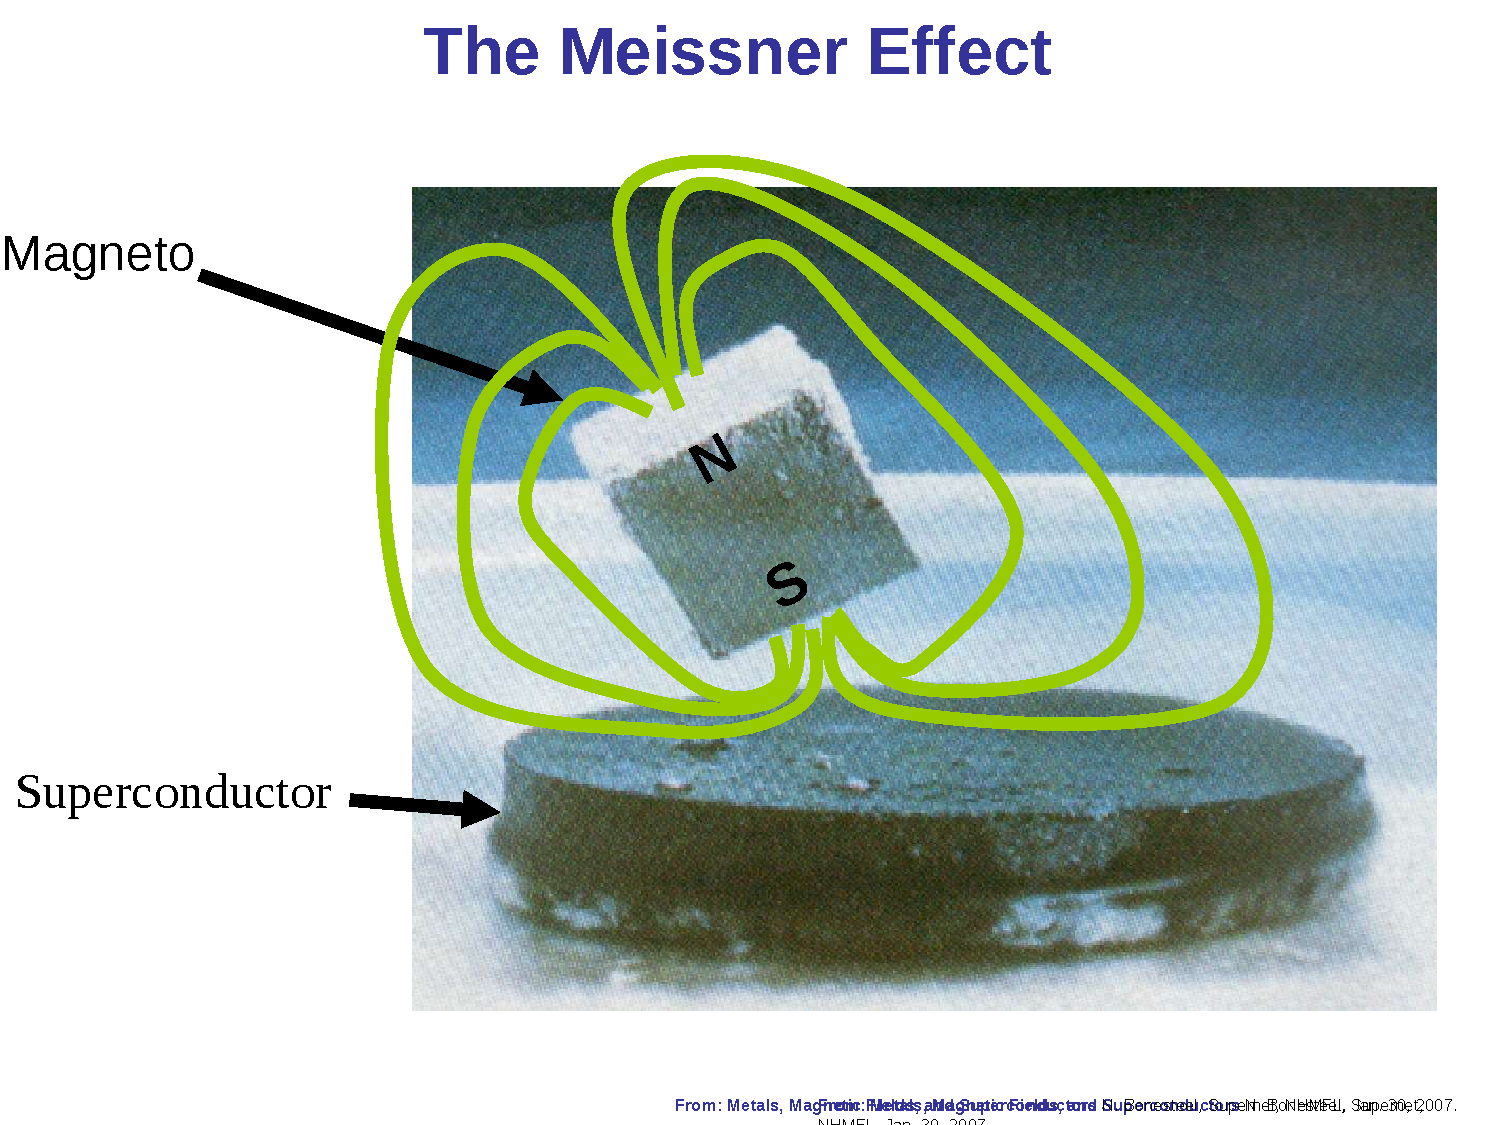
\includegraphics[width=\paperwidth]{meissner3}}
%\setbeamercovered{invisible}
\begin{frame}[plain]
\end{frame}
}
%%%%%%%%
%%%%%%%%
{
\usebackgroundtemplate{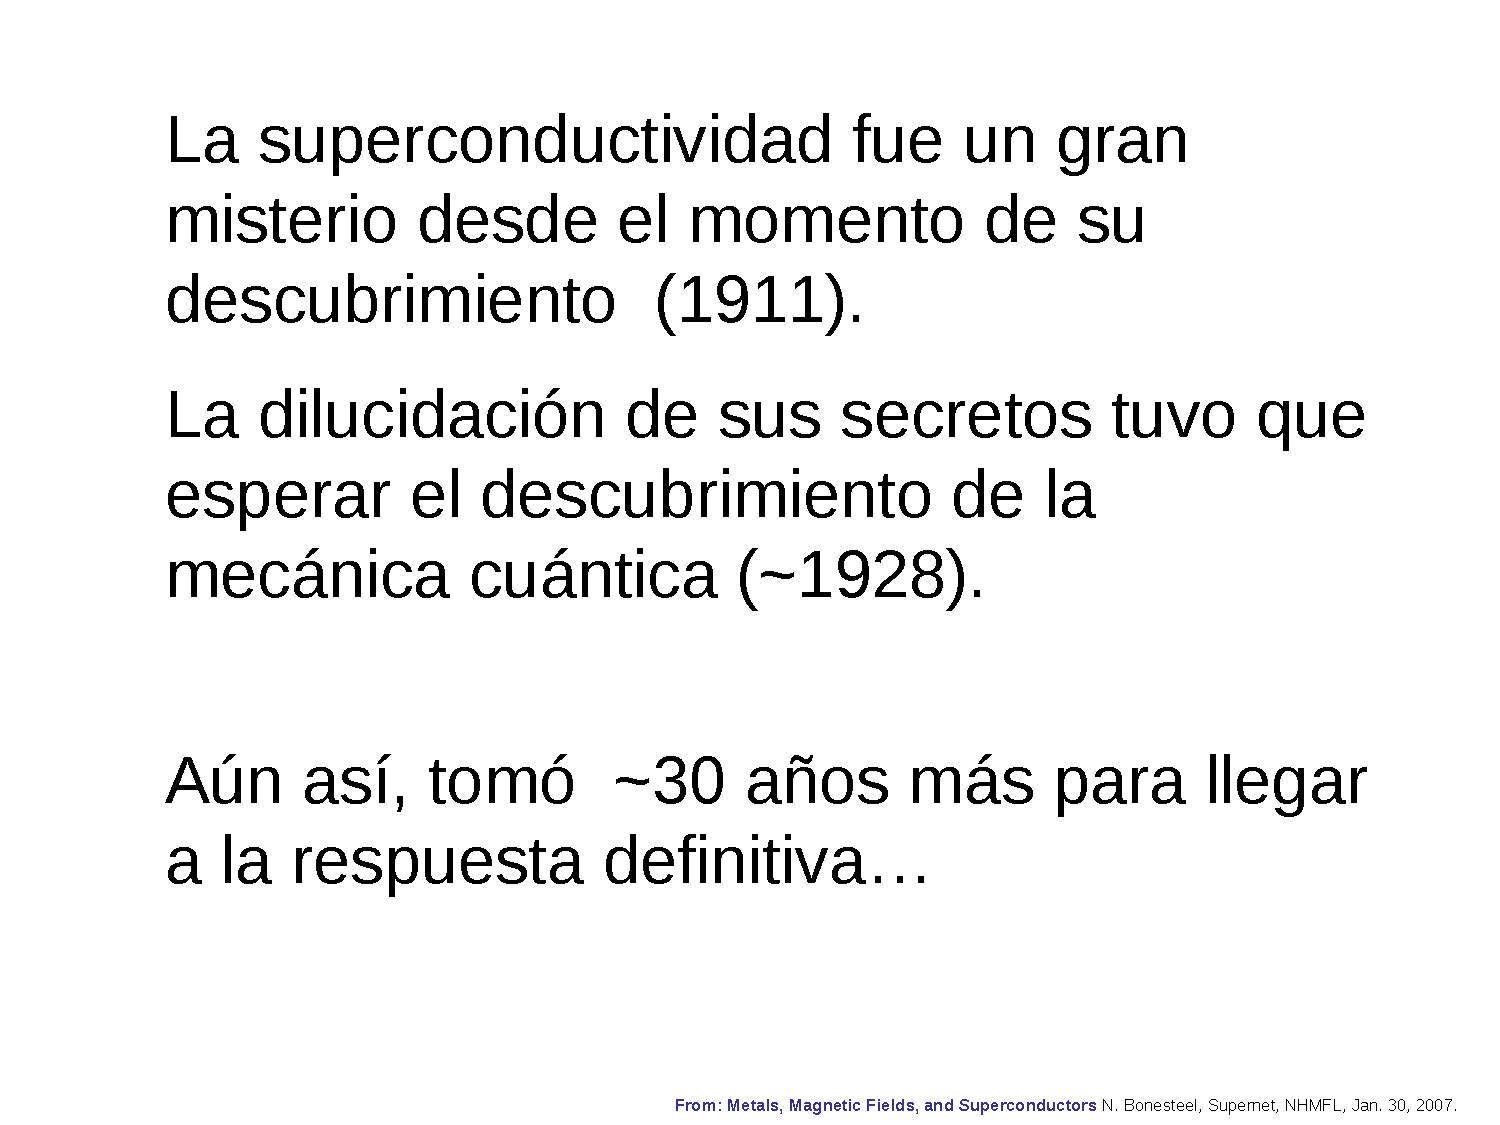
\includegraphics[width=\paperwidth]{mecanicacuantica}}
%\setbeamercovered{invisible}
\begin{frame}[plain]
\end{frame}
}
%%%%%%%%
\begin{frame}
  \frametitle{Tipos de partículas}
  Un sistema cuántico  tiene niveles de energía discretos que pueden ser ocupados secuencialmente dependiendo de si las partículas son:
  \begin{block}{fermiones}
    espín, en unidades semienteras de la constante de Planck reducida, denotada por $\hbar$
  \end{block}
  \begin{block}{bosones}
    espín en unidades enteras de $\hbar$.\footnote{El ``espín'' de la tierra es del orden de $10^{67}\hbar$.}
  \end{block}

\end{frame}
%%%%%%%%%%%%%
{
\usebackgroundtemplate{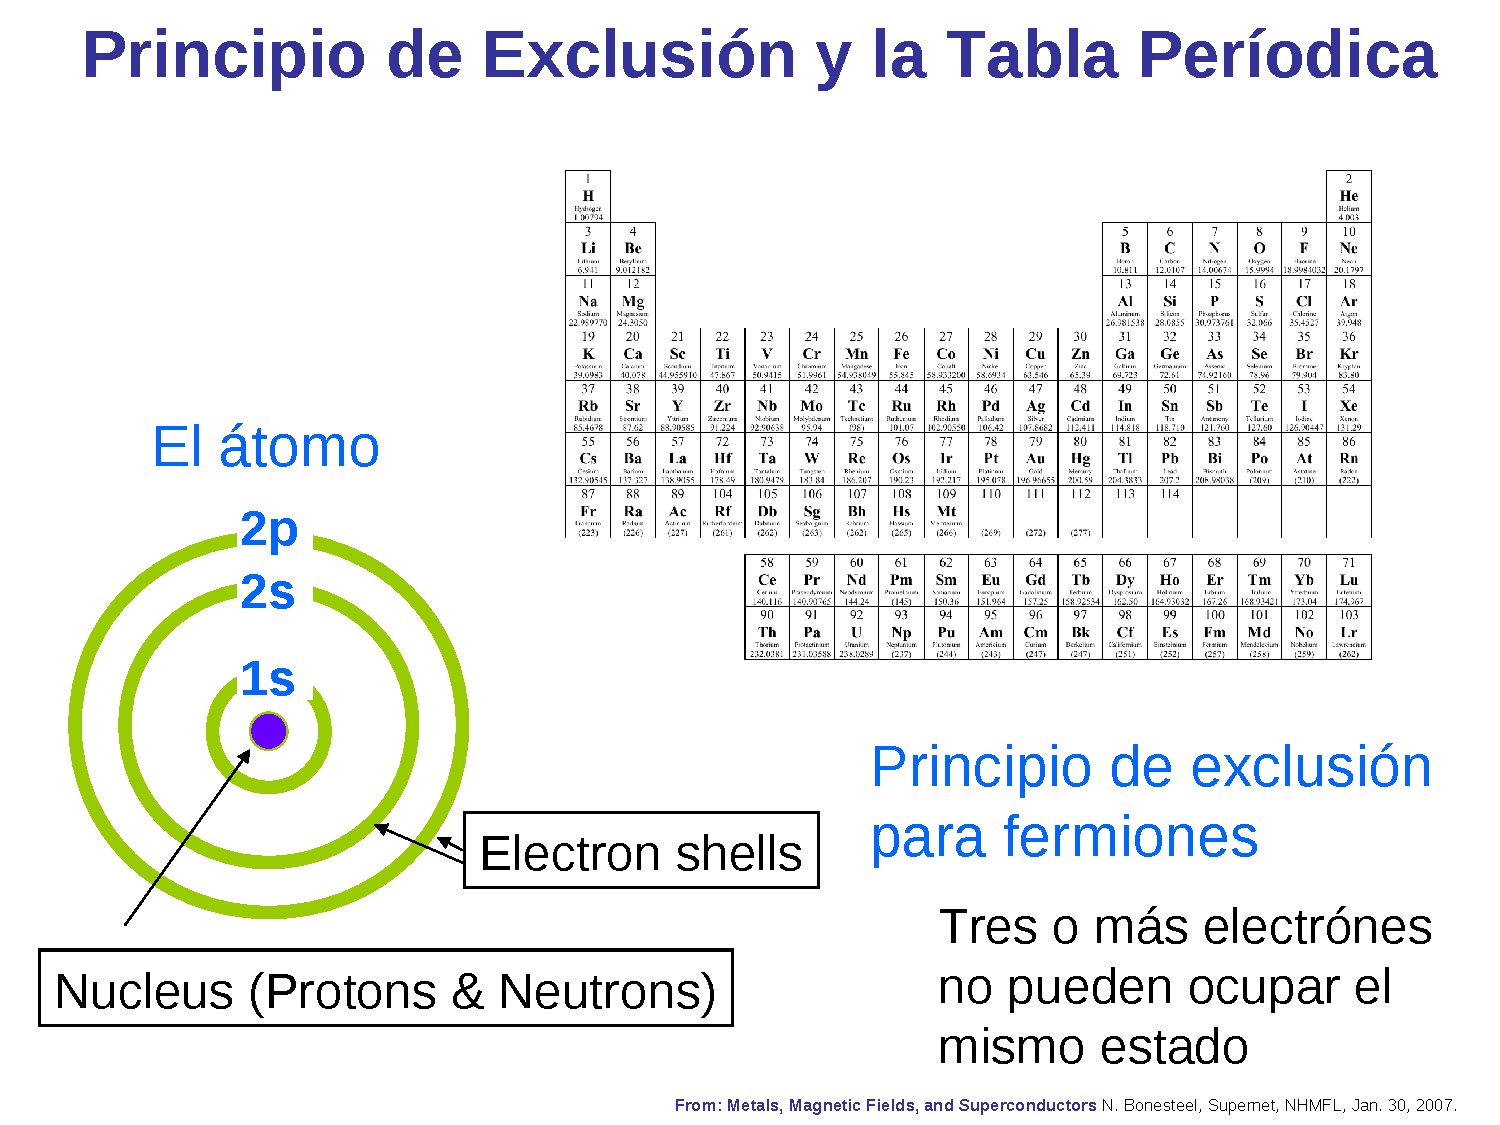
\includegraphics[width=\paperwidth]{ppiodeexclusion}}
%\setbeamercovered{invisible}
\begin{frame}[plain]
\end{frame}
}
%%%%%%%%
\begin{frame}
  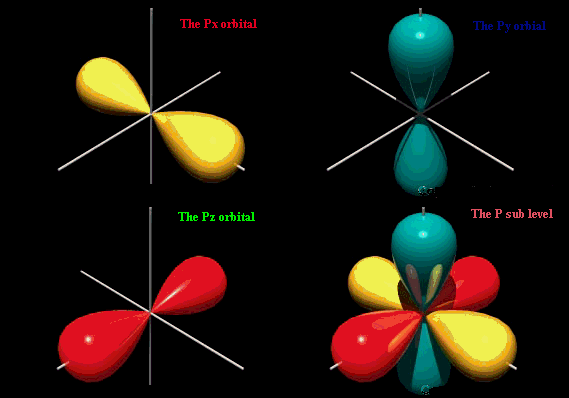
\includegraphics[scale=0.4]{porbital}
\end{frame}
%%%%%%%%%%%%%
%%%%%%%%%%%%%
{
\usebackgroundtemplate{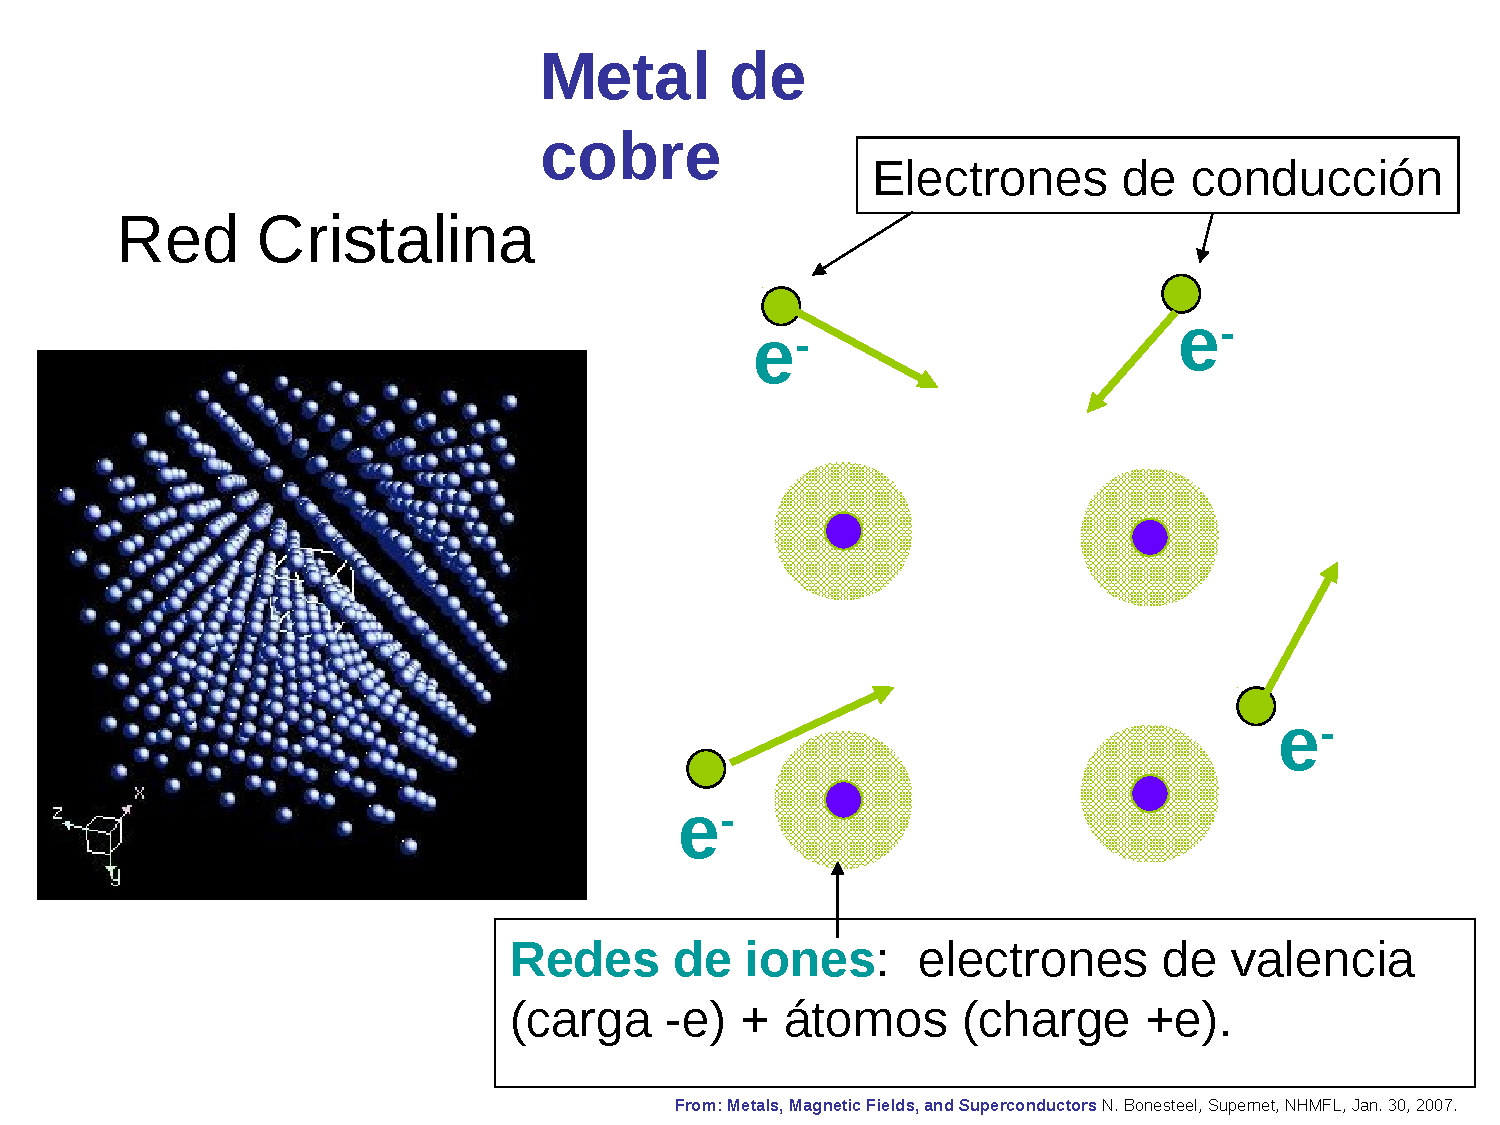
\includegraphics[width=\paperwidth]{nivelesmetal1}}
%\setbeamercovered{invisible}
\begin{frame}[plain]
\end{frame}
}
%%%%%%%%%%%%%
{
\usebackgroundtemplate{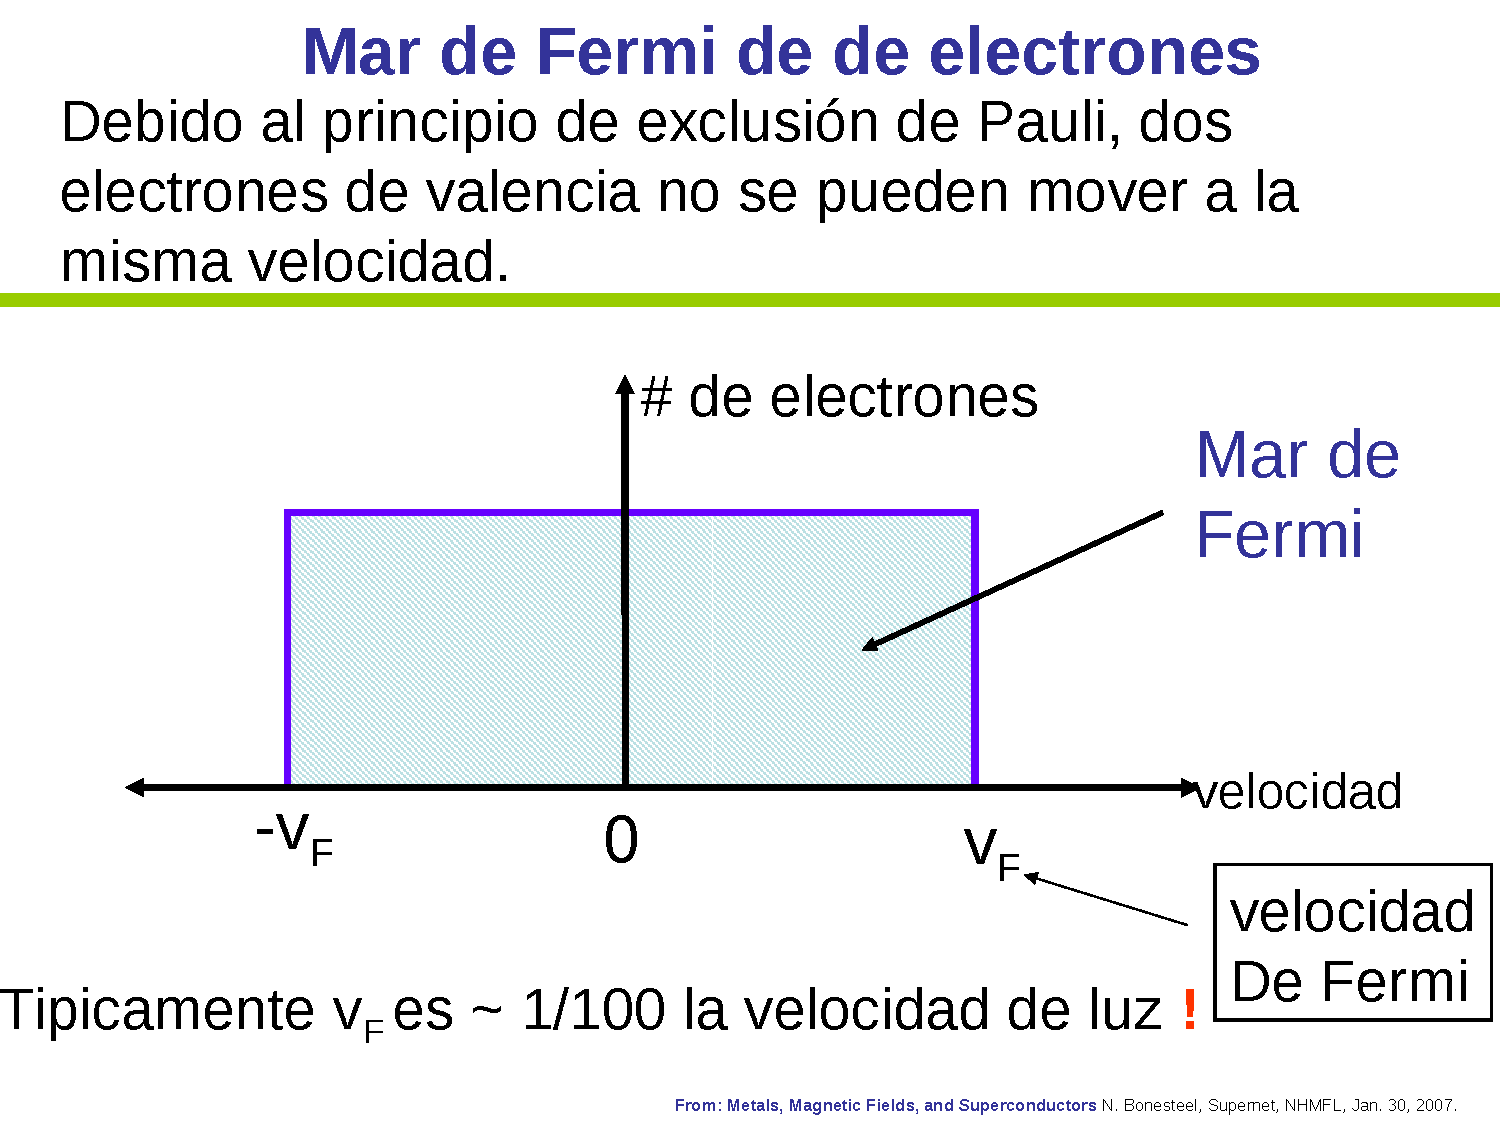
\includegraphics[width=\paperwidth]{nivelesmetal2}}
%\setbeamercovered{invisible}
\begin{frame}[plain]
\end{frame}
}
%%%%%%%%%%%%%
{
\usebackgroundtemplate{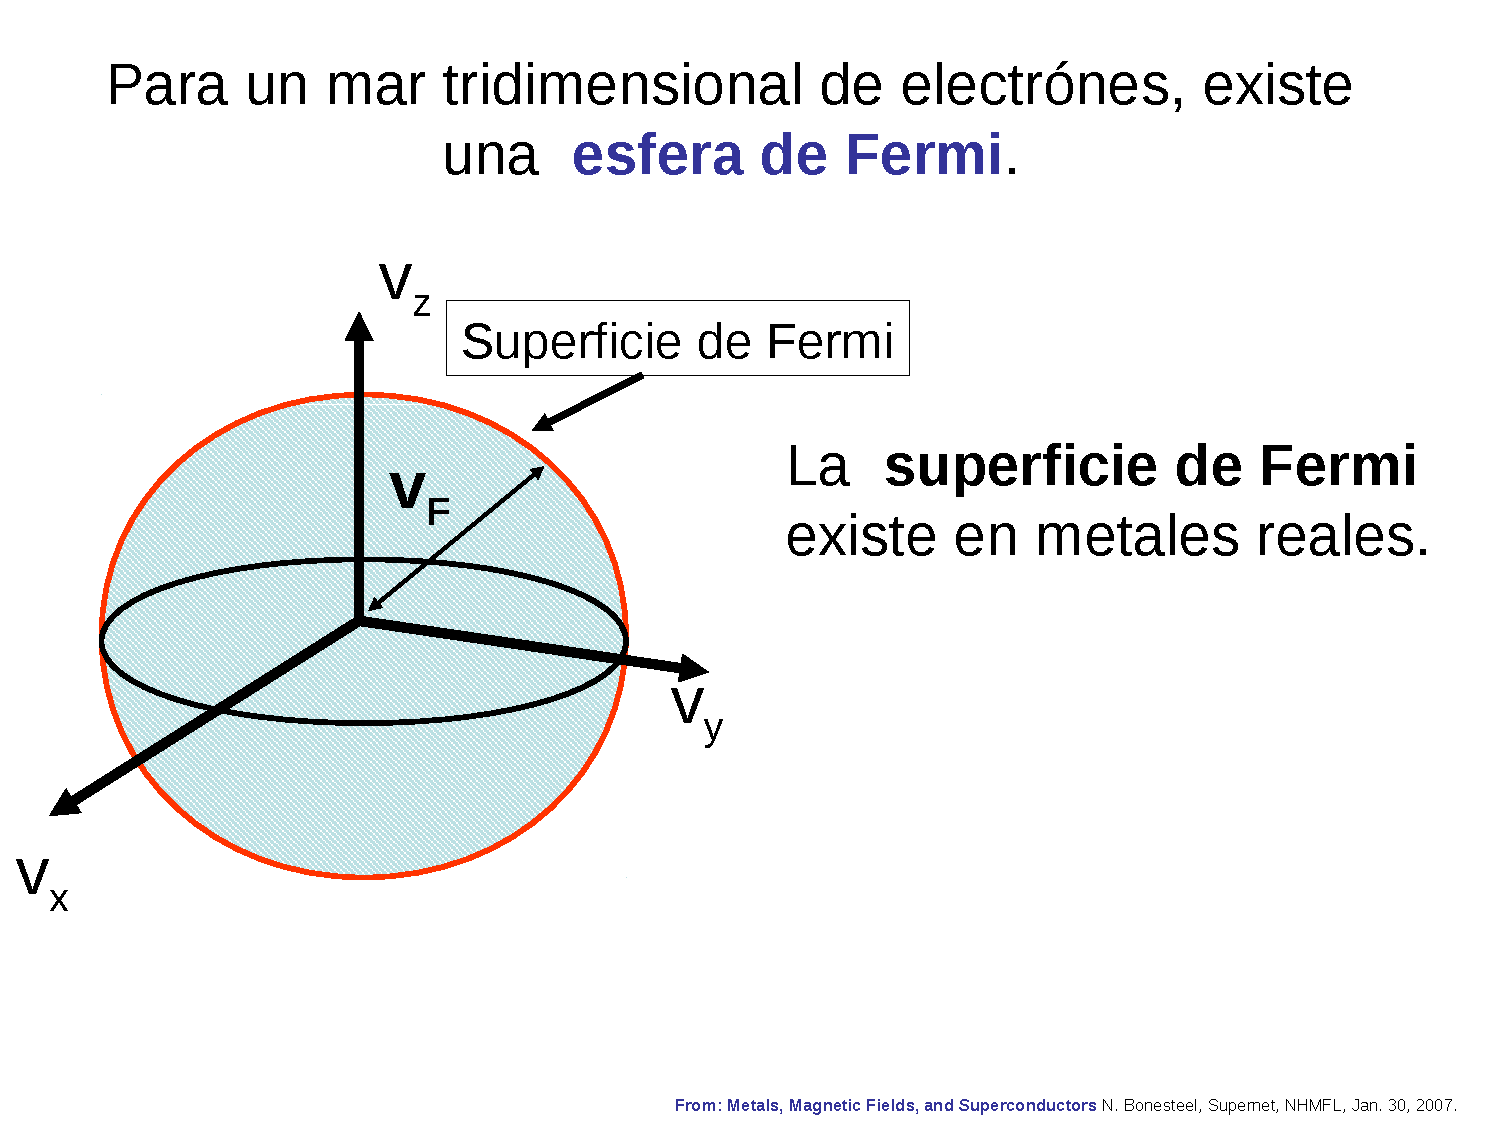
\includegraphics[width=\paperwidth]{nivelesmetal3a}}
%\setbeamercovered{invisible}
\begin{frame}[plain]
\end{frame}
}
%%%%%%%%%%%%%
{
\usebackgroundtemplate{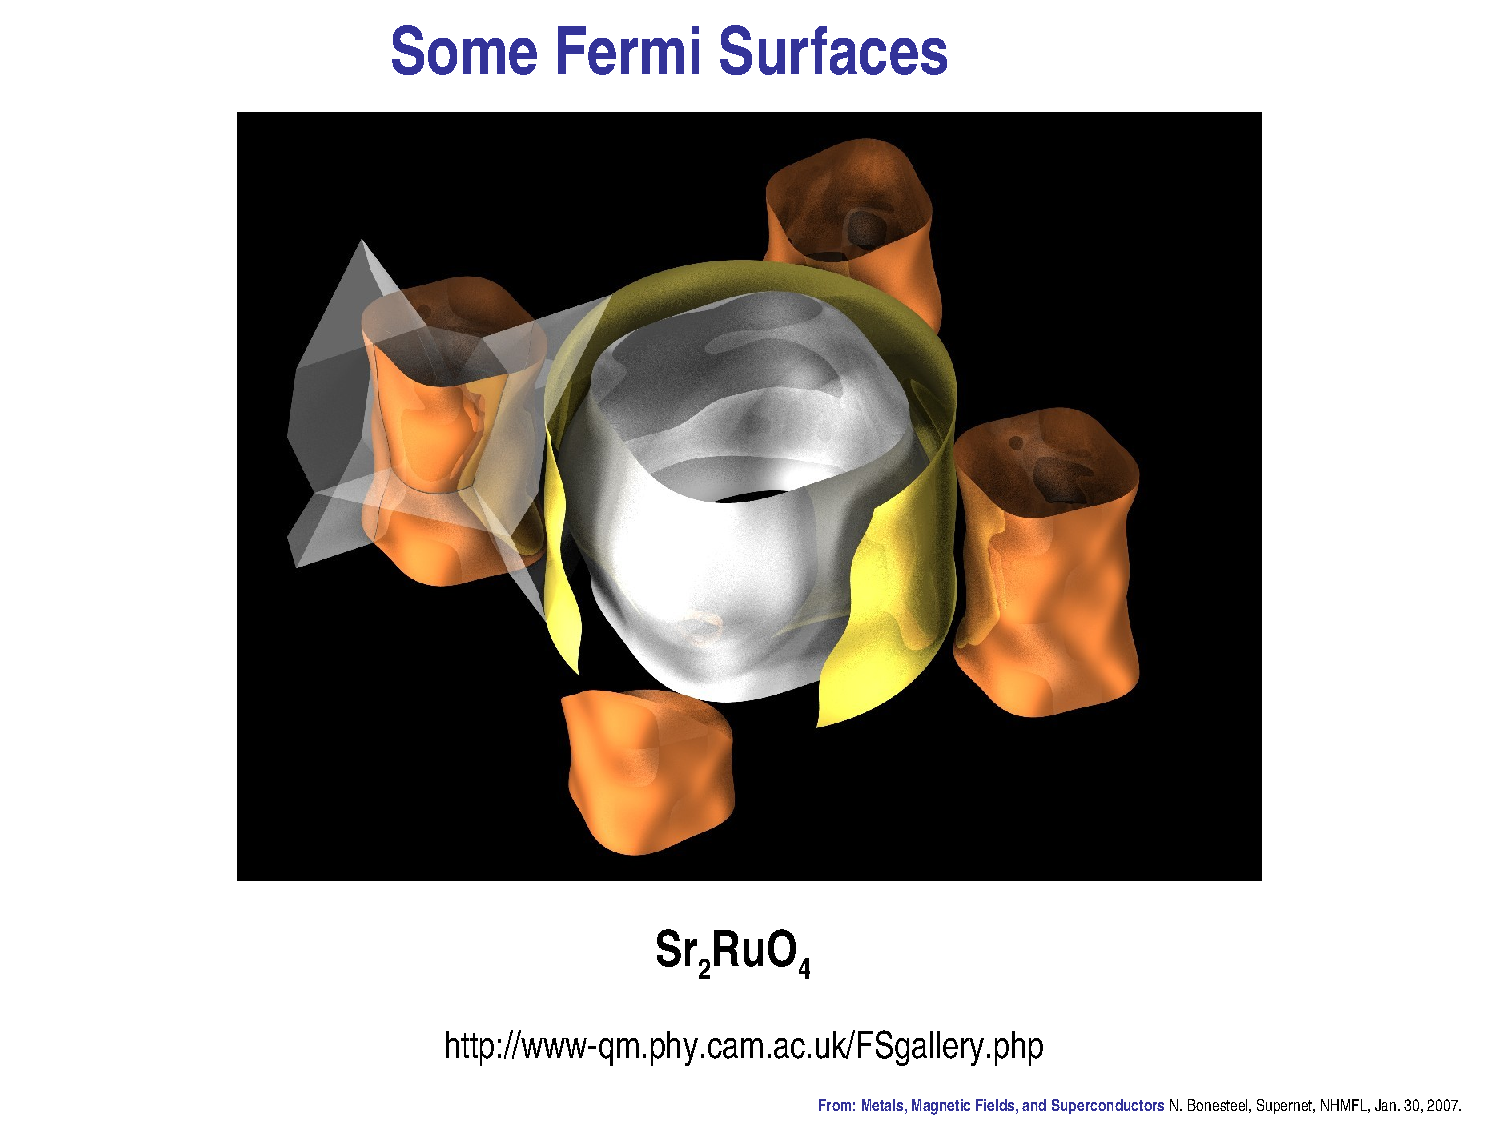
\includegraphics[width=\paperwidth]{nivelesmetal5}}
%\setbeamercovered{invisible}
\begin{frame}[plain]
\end{frame}
}
%%%%%%%%%%%%%
{
\usebackgroundtemplate{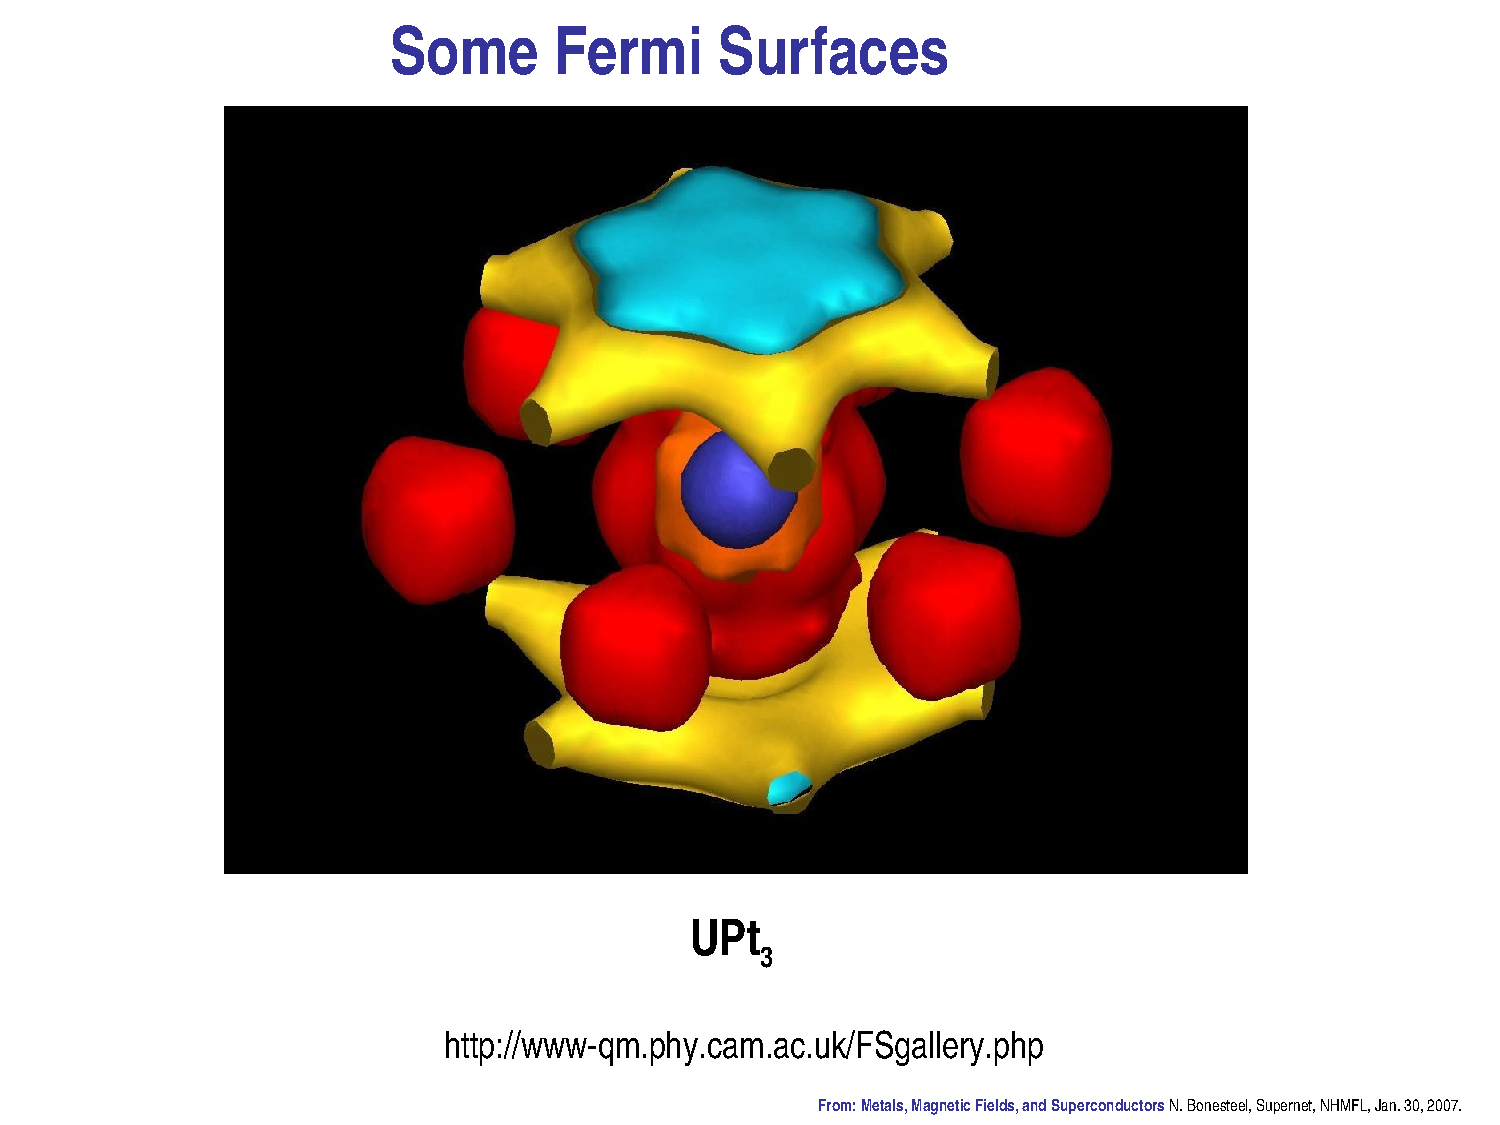
\includegraphics[width=\paperwidth]{nivelesmetal6}}
%\setbeamercovered{invisible}
\begin{frame}[plain]
\end{frame}
}

% \begin{frame}
%   \frametitle{Electrodinámica cuántica}
%   \begin{align*}
%   \psi(r)=|\psi(r)| e^{\theta(r)}  
%   \end{align*}
% \end{frame}

%%%%%%%Formación par de cooper
\begin{frame}
  \frametitle{Par de Cooper}
\only<1>{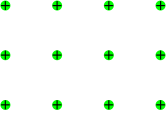
\includegraphics[scale=1.9]{pc1}}%
\only<2>{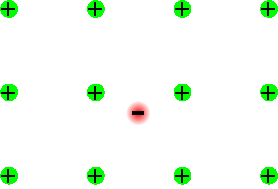
\includegraphics[scale=1.9]{pc2}}%
\only<3>{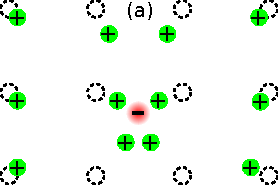
\includegraphics[scale=1.9]{pc3}}%
\only<4>{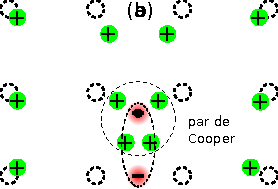
\includegraphics[scale=1.9]{pc4}}
\end{frame}

%%%%%%%%%%%%%
{
\usebackgroundtemplate{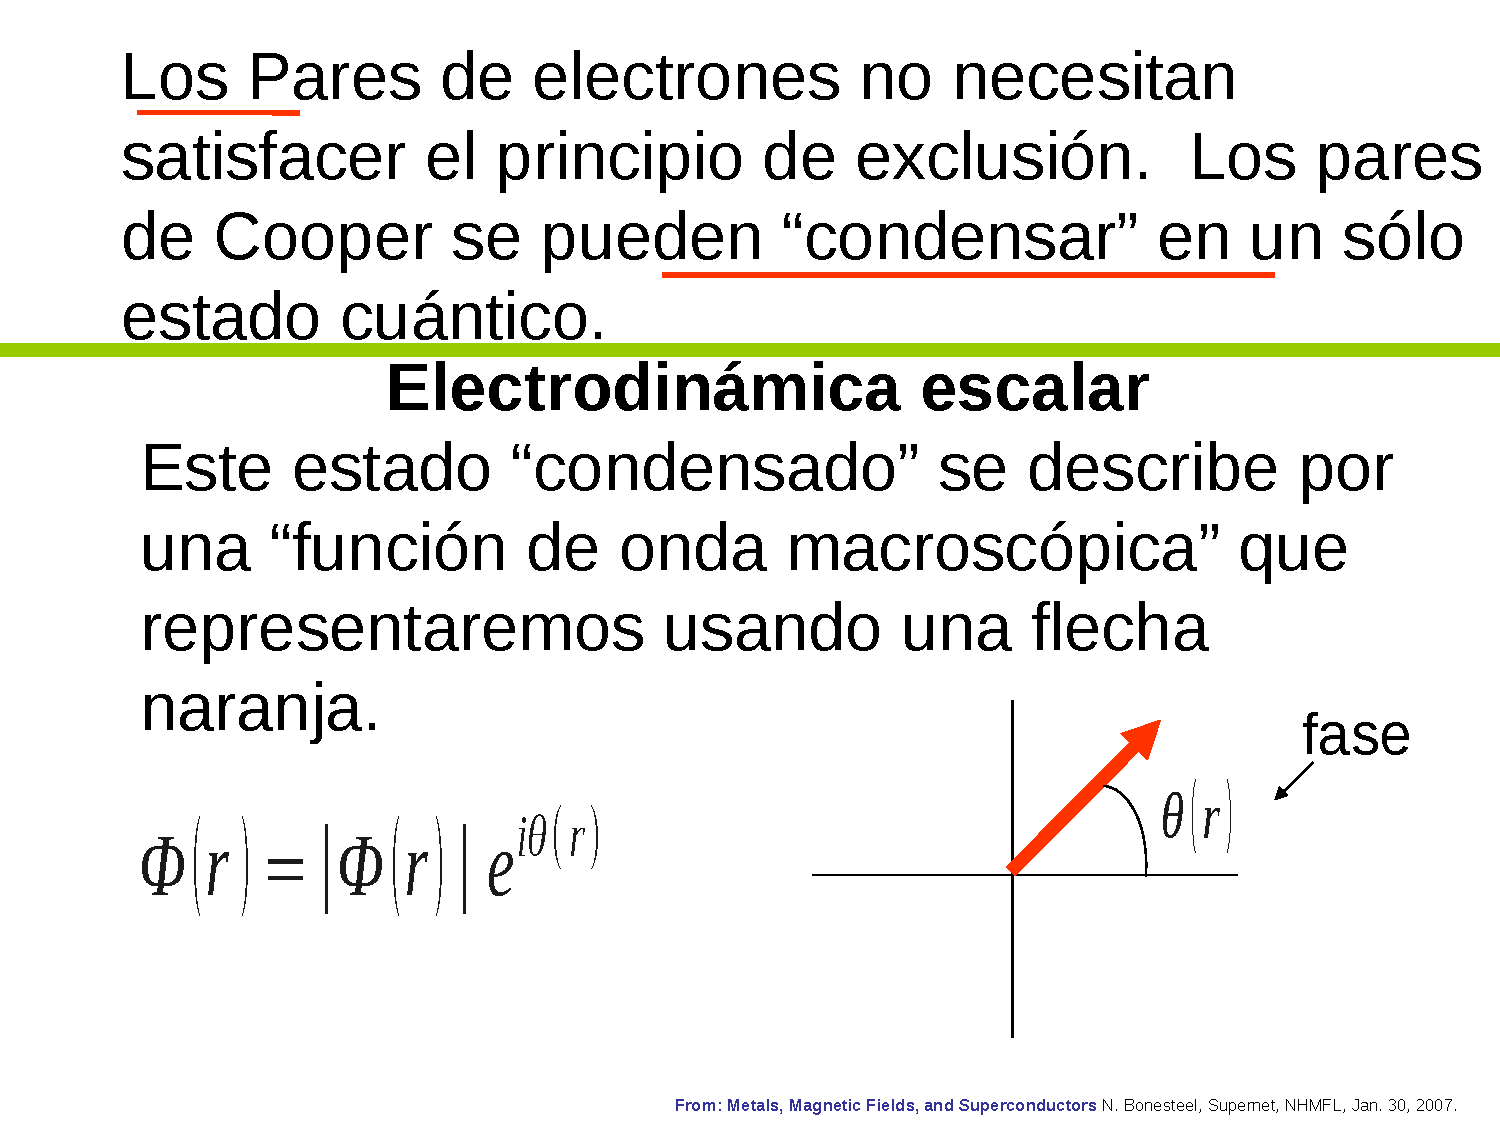
\includegraphics[width=\paperwidth]{scalarqed}}
%\setbeamercovered{invisible}
\begin{frame}[plain]
\end{frame}
}

\begin{frame}
  \frametitle{Ruptura espontánea de la simetría}
  \begin{figure}
  \centering
  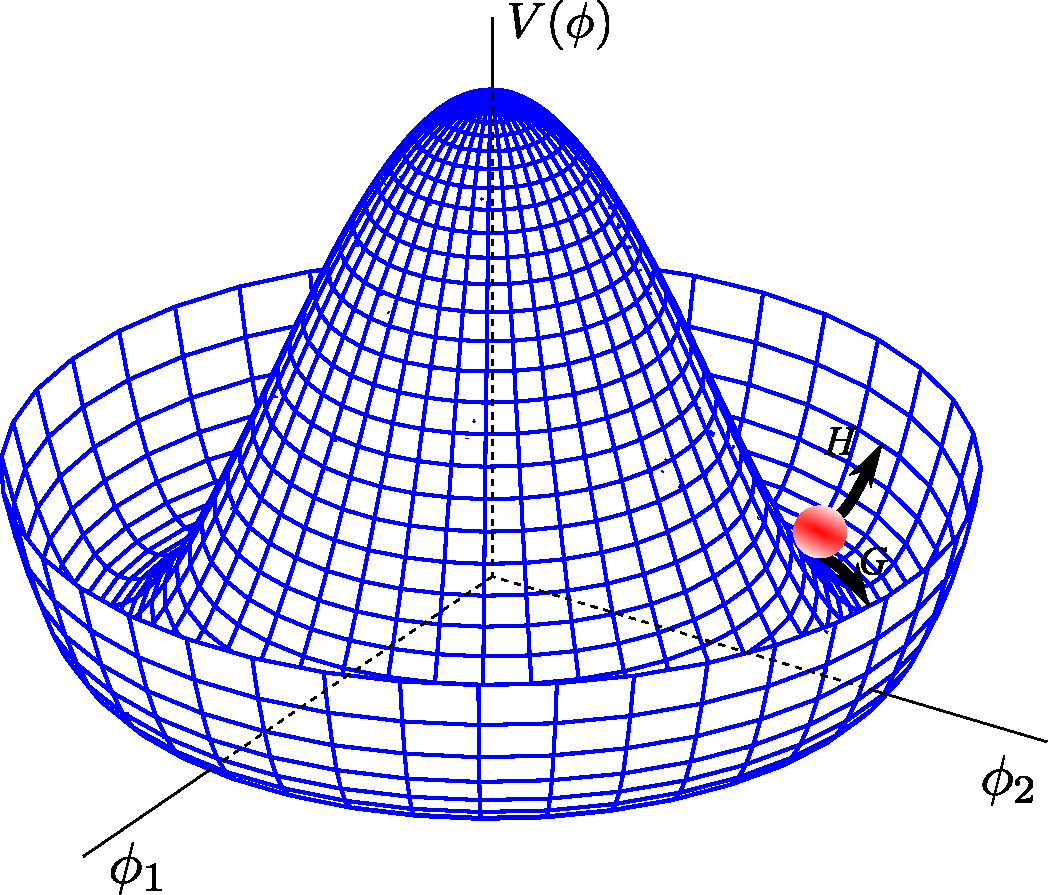
\includegraphics[scale=0.5]{mexicanhat}
  \caption{Potencial para un campo escalar complejo}
  \label{fig:mexicanhat}
\end{figure}
\end{frame}
%%%%%%%%%%%%%
{
\usebackgroundtemplate{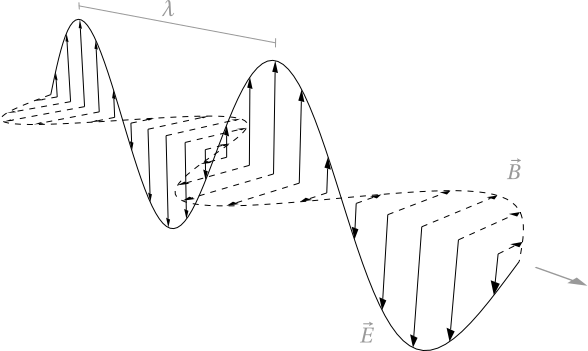
\includegraphics[width=\paperwidth]{Electromagnetic_wave}}
%\setbeamercovered{invisible}
\begin{frame}[plain]
\end{frame}
}

%%%%%%%%%%%%%
{
\usebackgroundtemplate{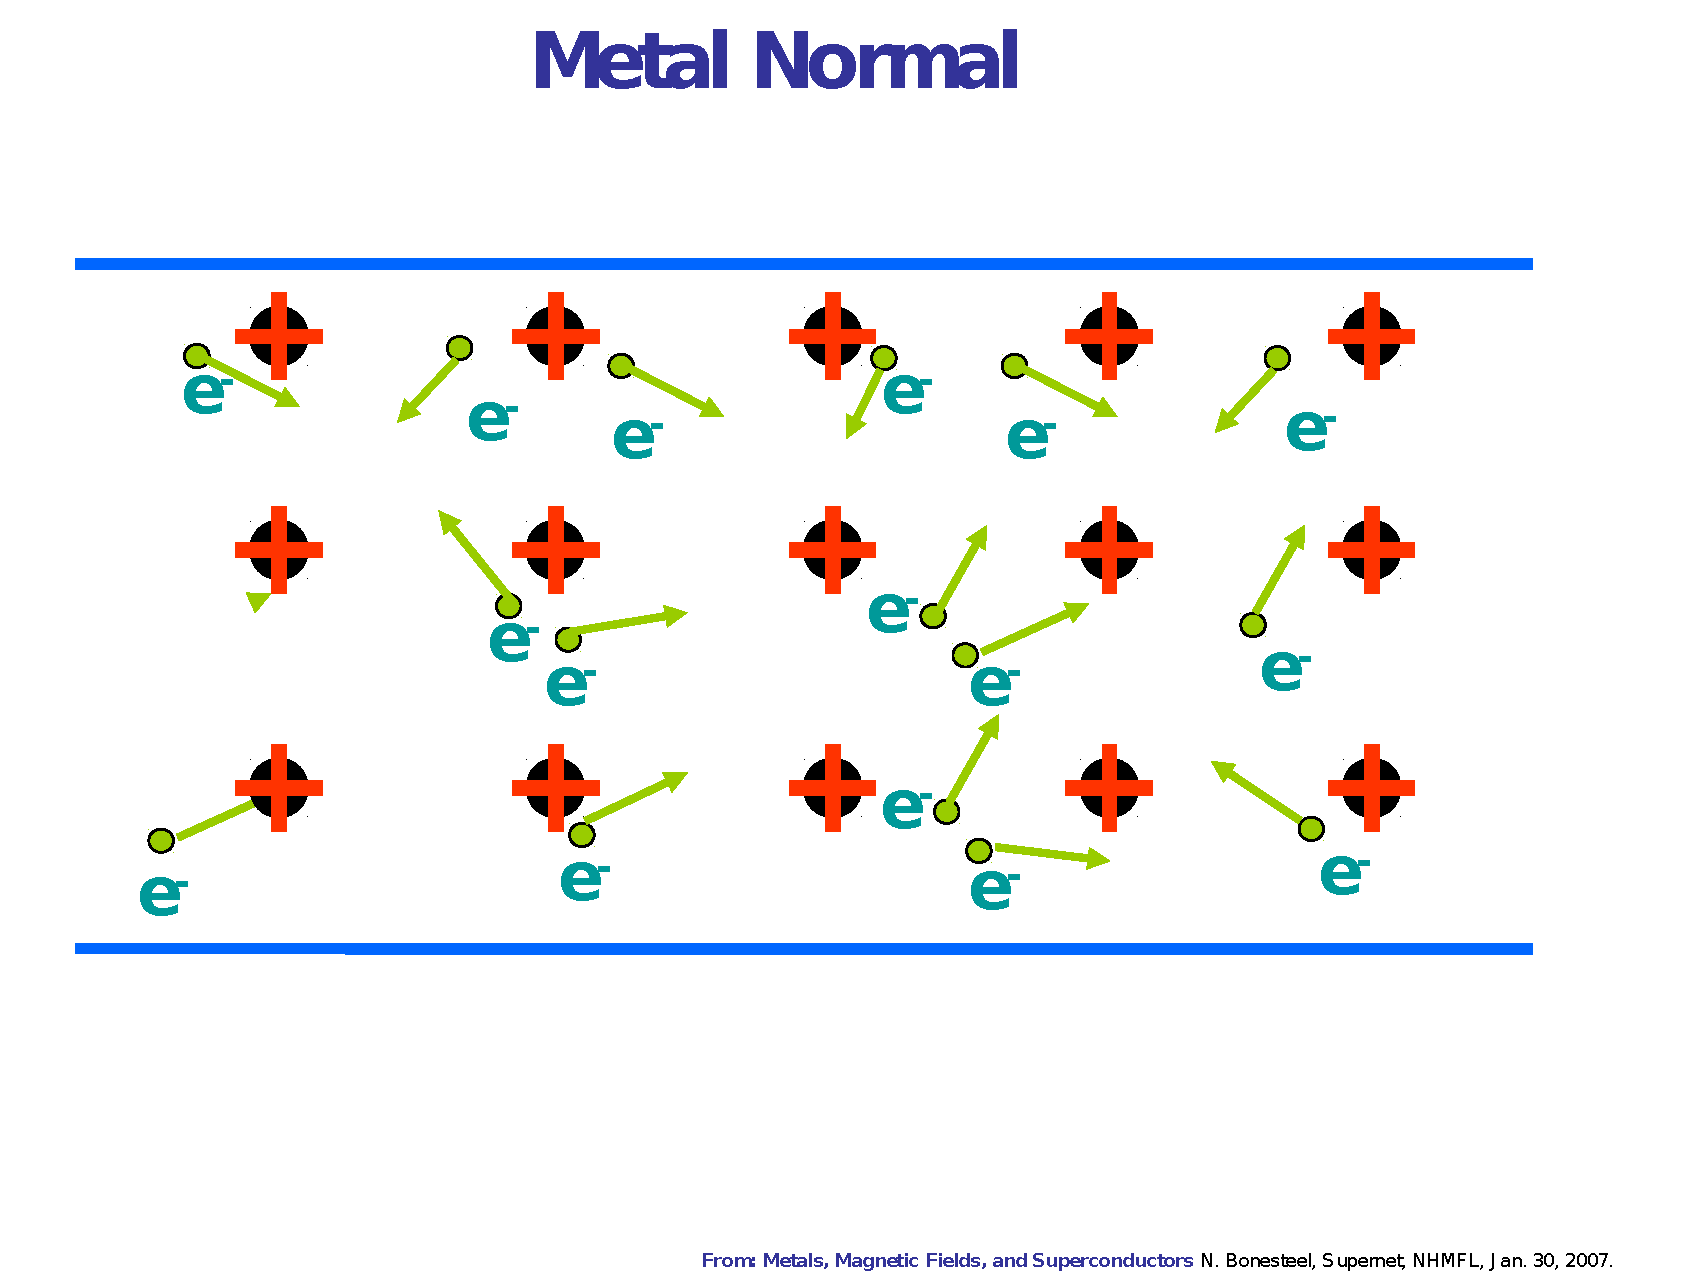
\includegraphics[height=\paperheight]{normalmetal1}}
%\setbeamercovered{invisible}
\begin{frame}[plain]
\end{frame}
}
%%%%%%%%%%%%%
%%%%%%%%%%%%%
{
\usebackgroundtemplate{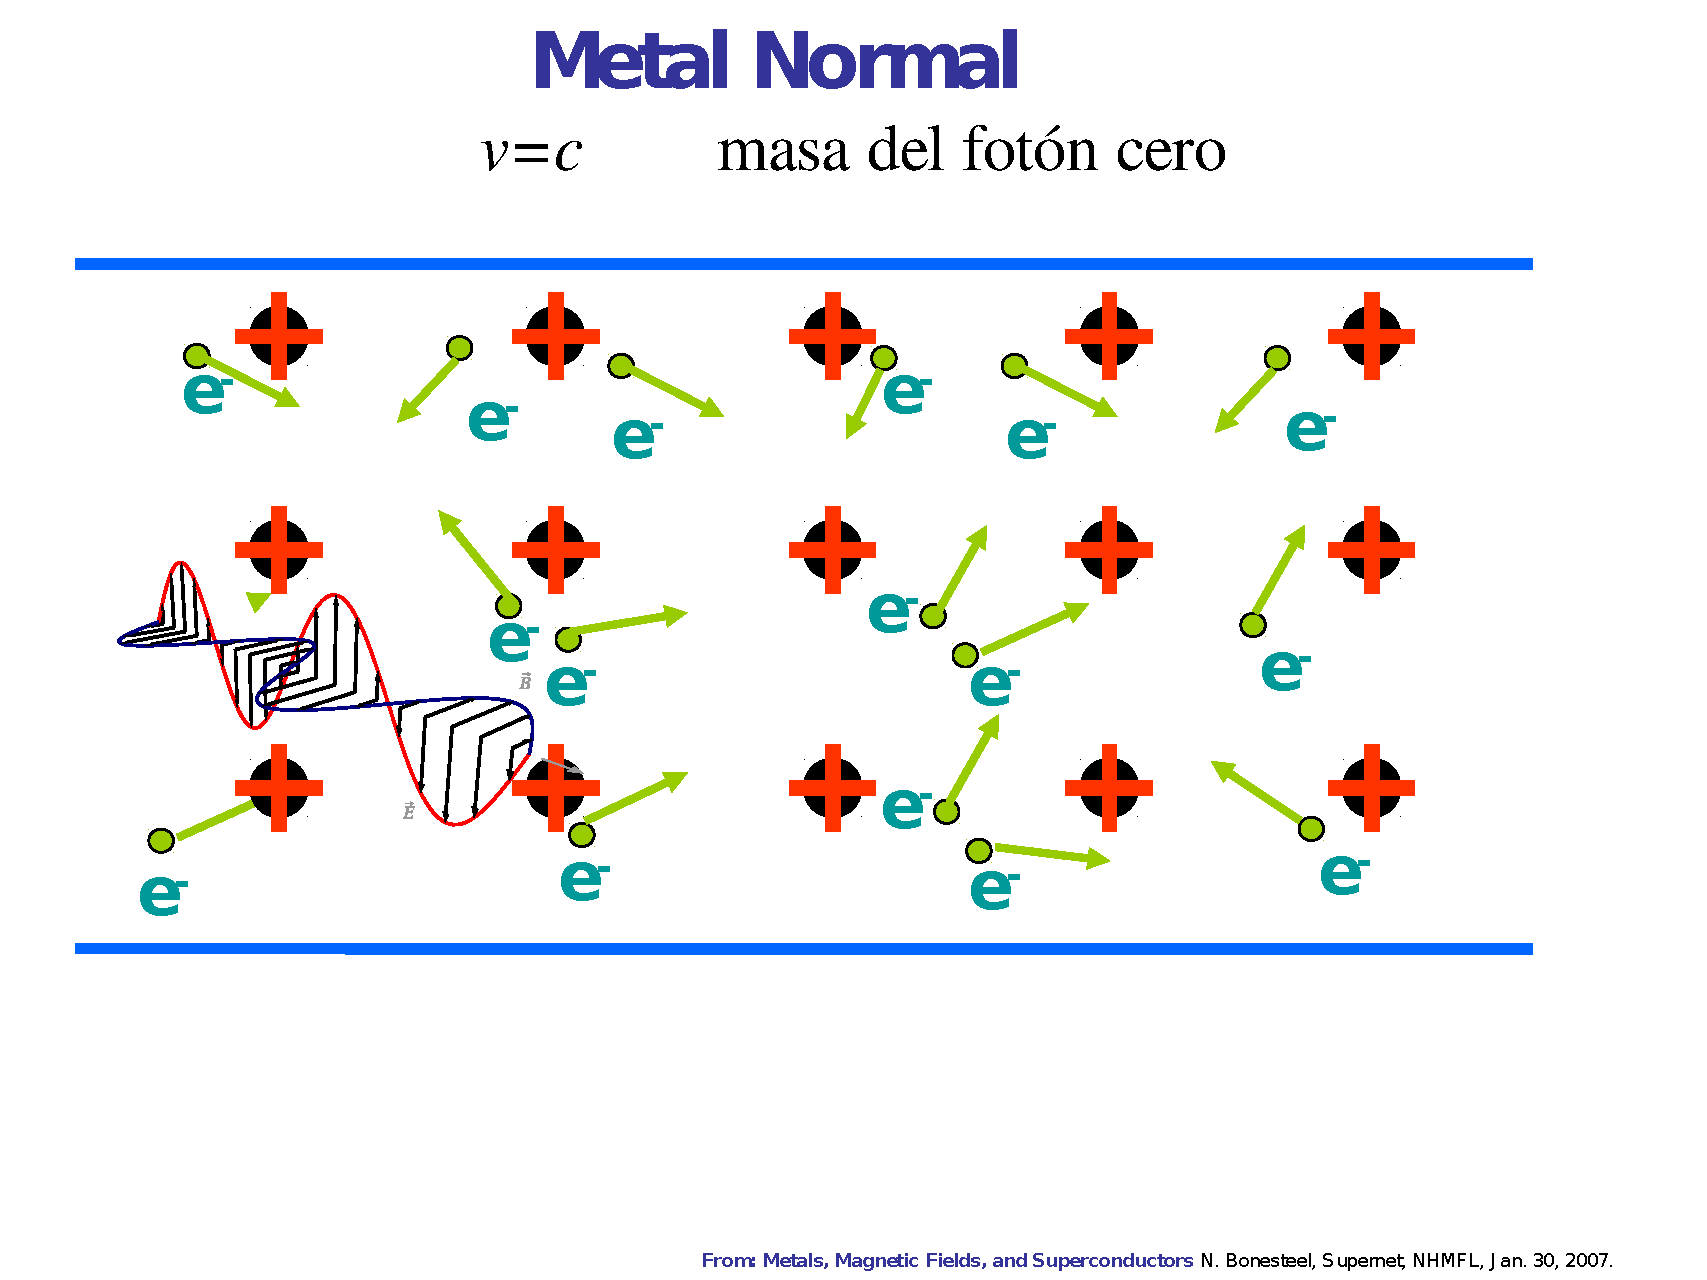
\includegraphics[width=\paperwidth]{normalmetal2}}
%\setbeamercovered{invisible}
\begin{frame}[plain]
\end{frame}
}
%%%%%%%%%%%%%
{
\usebackgroundtemplate{\includegraphics[width=\paperwidth]{superconductorflecha1}}
%\setbeamercovered{invisible}
\begin{frame}[plain]
\end{frame}
}
%%%%%%%%%%%%%
{
\usebackgroundtemplate{\includegraphics[width=\paperwidth]{superconductorflecha2}}
%\setbeamercovered{invisible}
\begin{frame}[plain]
\end{frame}
}

%%%%%%%%%%%%%
{
\usebackgroundtemplate{\includegraphics[width=\paperwidth]{weakall0}}
%\setbeamercovered{invisible}
\begin{frame}{$W^\pm,\ Z^0$: Masa \alert{real} o emergente?\phantom{, \alert{Higgs} or not Higgs?}}
\qquad
\vspace{6cm}
\begin{itemize}
\item ``Fotones'' con masa
\item Interacción de corto alcance
\item Éter electrodébil
\end{itemize}
\end{frame}
}
%%%%%%%%%%%%%
{
\usebackgroundtemplate{\includegraphics[width=\paperwidth]{weakall1}}
%\setbeamercovered{invisible}
\begin{frame}{$W^\pm,\ Z^0$: Masa real o \alert{emergente}?\phantom{, \alert{Higgs} or not Higgs?}}
\qquad
\vspace{6cm}
\begin{itemize}
\item ``Fotones'' con masa
\item Interacción de corto alcance
\item Éter electrodébil
\end{itemize}
\end{frame}
}
%%%%%%%%%%%%%
{
\usebackgroundtemplate{\includegraphics[width=\paperwidth]{weakall2}}
%\setbeamercovered{invisible}
\begin{frame}{$W^\pm,\ Z^0$: Masa real o \alert{emergente}?, \alert{Higgs} or not Higgs?}
\qquad
\vspace{6cm}
\begin{itemize}
\item ``Fotones'' con masa
\item Interacción de corto alcance
\item Éter electrodébil
\end{itemize}
\end{frame}
}



\begin{frame}
  \frametitle{Superconductividad electrodébil}
  \begin{itemize}
  \item Las interacciones débiles han resultados ser fuerzas de corto alcance, mediadas por nuevos fotones llamados $W$ y $Z$ que son bastante masivos
  \item Interpretadas como masas emergentes implican que:
    \begin{itemize}
    \item Vivimos en un estado de superconductiviad electrodébil! $T_c=10^{15}\ $GeV.
    \item Existe un éter electrodébil que permea todo el universo
    \item No entendemos el origen de las flechas (al igual que en superconductividad electromagnética a altas temperaturas)
    \end{itemize}
  \end{itemize}

  \begin{block}{Predicción}
 Aunque no podemos acceder directamente a las componentes del condensado que se comen el $W$ y el $Z$ para adquirir masa, existe al menos otra componente del condensado que se debe materializar como partícula independiente y nueva
 \begin{center}
   La partícula de Higgs!
 \end{center}
  \end{block}

\url{http://gfif.udea.edu.co/downloads/paper.pdf}
\end{frame}





%%%%%%%%%%%
\begin{frame}
\only<1>{\includegraphics[scale=0.4]{smblocks1.png}}%
%\only<2>{\includegraphics[scale=0.7]{smblocks2}}%
%\only<3>{\includegraphics[scale=0.7]{smblocks3}}%
%\only<4>{\includegraphics[scale=0.7]{smblocks4}}%
%\only<5>{\includegraphics[scale=0.7]{smblocks5}}%

\end{frame}

\begin{frame}
\frametitle{Standard Model: particles}
\only<1>{\includegraphics[bb=30 0 0 200,scale=0.75]{sm01a}}%
\only<2>{\includegraphics[bb=30 0 0 200,scale=0.75]{sm01b}}%
\only<3>{\includegraphics[bb=30 0 0 200,scale=0.75]{sm01}}%
\only<4>{\includegraphics[bb=30 0 0 200,scale=0.75]{sm02}}%
\only<5>{\includegraphics[bb=30 0 0 200,scale=0.75]{sm03}}%
\only<6>{\includegraphics[bb=30 0 0 200,scale=0.75]{sm04}}%
\only<7>{\includegraphics[bb=30 0 0 200,scale=0.75]{sm05}}%
\only<8>{\includegraphics[bb=30 0 0 200,scale=0.75]{sm06}}%
\only<9>{\includegraphics[bb=30 0 0 200,scale=0.75]{sm07}}%
\only<10>{\includegraphics[bb=30 0 0 200,scale=0.75]{sm08}}%
\invisible<1-9>{
  \begin{block}{SM particles}
    +Gauge invariance+Lorentz Invariance$\to$Lagrangian (interactions)   
  \end{block}

}
\end{frame}
%%%%%%%%%%%%%%%%


%%%%%%%%%%%%%%%%%%%
\begin{frame}
  La luz penetrando en un metal que a nivel microscópio corresponde a rayos dispersandoes a la velocidad de la luz, se puede entender como un efecto macróscopico de un fotón masivo. Igual la luz viaja en el vacío
\end{frame}
\begin{frame}
  Pero el vacío podría estar lleno de campos
\end{frame}
\begin{frame}
  El campo es un concepto difícil, Es algo que ocupa lugar y transporta energía. Pero ante de todo ...  
\end{frame}
\begin{frame}
  Discutir la masa del protón
\end{frame}
\begin{frame}
  Hablar de superconductivada
\end{frame}
\begin{frame}
  Mecanismo de Higgs
\end{frame}




%%%%%%%%%%%%%%%%%%%%%
\begin{frame}
  \frametitle{Standard Model Lagrangian \tiny{(simplified version)}}
  \only<1>{\includegraphics[scale=0.43]{smtshirtzoom1}}%
  \only<2>{\includegraphics[scale=0.43]{smtshirtzoom2}}%
\end{frame}
%%%%%%%%%%%%%%%%%%%%
\begin{frame}
  \frametitle{Higgs production and decay}
  \begin{block}{Gluon fusion}
    \includegraphics[scale=0.4]{gluonfusion}
  \end{block}
  \begin{block}{Golden channel}
    \includegraphics[scale=0.4]{golden_channel}
  \end{block}
\end{frame}
%%%%%%%%%%
{
\usebackgroundtemplate{\includegraphics[width=\paperwidth]{fermionspc}}
\begin{frame}[plain]
\end{frame}
}
{
\usebackgroundtemplate{\includegraphics[width=\paperwidth]{fermionspcnu}}
\begin{frame}[plain]
\end{frame}
}
%%%%%%%%
%%%%%%%%%%%%%%%%%%%%%%%%%%%%%%%%%%%%%%%%%%%%%%%
%%%%%%%%%%%%%%%%%%%%%%%%%%%%%%%%%%%%%%%%%%%%%%%%
%%%%%% DARK SIDE %%%%%%%%%%%%%%%%%%%%%%%%%%%%%%%
%%%%%%%%%%
{
\setbeamercovered{invisible}
\begin{frame}
\frametitle{Energy budget of the Universe}
\alert{$\Lambda$CDM}: Cosmological Constant + Cold Dark Matter:

\vspace{-0.5cm}
\begin{columns}
  \begin{column}{0.55\textwidth}
    \begin{itemize}
    \item<1-> Stars y galaxies are only $\sim 0.4\%$
    \item<2-> Rest of ordinary matter $\sim 3.5\%$
      \begin{itemize}
      \item<2-> neutrinos $\sim 0.1-1\%$
      \item<2-> electrones, protones, y neutrones
      \end{itemize}
    \item<3-> Dark Matter $\sim 23\%$
    \item<4-> Dark Energy $\sim 73\%$

      \invisible<1-3>{\includegraphics[scale=0.5]{nobel-u_small}}

      \tiny{A. Riess, S. Perlmutter, B. Schimdt}
    \item<5-> Anti-Matter $\sim 0\%$
    \end{itemize}
  \end{column}
  \begin{column}{0.45\textwidth}
\vspace{0.5cm}

    \only<1>{\includegraphics[scale=0.5]{energybudgetstars}}%
\only<2>{\includegraphics[scale=0.5]{energybudgetnonluminous}}%
\only<3>{\includegraphics[scale=0.5]{energybudgetDM}}%
\only<4->{\includegraphics[scale=0.5]{energybudgetDE}}%
  \end{column}
\end{columns}
\end{frame}
}
%%%%%%%
{
 \setbeamertemplate{blocks}[rounded][shadow=false]
%http://astrohow.org/astroconcepts/bullet.html
\usebackgroundtemplate{\includegraphics[width=\paperwidth]{bullet}}
\setbeamercovered{invisible}
\begin{frame}
\frametitle{Bullet cluster 1E 0657-558 (2006) \tiny{two colliding clusters of galaxies}}
  \only<2>{\includegraphics[scale=0.5]{galaxycollisionbefore}}%
  \only<3>{\includegraphics[scale=0.5]{galaxycollision}}%
  \only<4>{\includegraphics[scale=0.5]{galaxycollisionafter}}%
  \only<6>{
    \begin{block}{WIMP Dark Matter}
      \begin{center}
        \color{blue} Weakly Interacting Massive Particle
      \end{center}

Stable heavy particle produced in early universe, left over from near--complete annihilation
\begin{itemize}
\item  WIMP miracle
\begin{align*}
  \Omega_{\text{DM}}=\frac{0.756(n+1)x_f^{n+1}}{g^{1/2}\sigma_{\text{ann}}}
\frac{3s_0}{8\pi H_0^2}\approx \frac{\alpha^2/(\alert{1\;\text{TeV}})}{\sigma_{\text{ann}}}
\end{align*}

\end{itemize}

    \end{block}
}
\end{frame}
}
%%%%%%%%%%%%%%%%%
%%%%%%%%%%
\begin{frame}
\only<1>{\includegraphics[bb=20 0 0 600,scale=0.44]{experimentos}}%
\only<2>{\includegraphics[bb=20 0 0 600,scale=0.44]{experimentosfermi}}%
\only<3>{\includegraphics[bb=20 0 0 600,scale=0.44]{experimentospamela}}%
\only<4>{\includegraphics[bb=20 0 0 600,scale=0.44]{experimentosams}}%
\only<5>{\includegraphics[bb=20 0 0 600,scale=0.44]{experimentoslhc}}%
\only<6>{\includegraphics[bb=20 0 0 600,scale=0.44]{experimentosminos}}%
\only<7>{\includegraphics[bb=20 0 0 600,scale=0.44]{experimentossk}}%
\only<8>{\includegraphics[bb=20 0 0 600,scale=0.44]{experimentosgs}}%
\only<9>{\includegraphics[bb=20 0 0 600,scale=0.44]{experimentosantares}}%
\only<10>{\includegraphics[bb=20 0 0 600,scale=0.44]{experimentosicecube}}%
\end{frame}
%%%%%%%%%%%%%%%%%%%%%%
\begin{frame}
  \includegraphics[scale=0.4]{IceCube-Eiffel}
\end{frame}
%%%%%%%%%

{
%DEBUG:
\usebackgroundtemplate{\includegraphics[width=\paperwidth]{lhcm}}
\setbeamertemplate{blocks}[rounded][shadow=false]
\setbeamercovered{invisible}
 \begin{frame}

\begin{columns}
\column{.48\textwidth}
   \begin{block}<2->{Tevatron}
     \rowcolors{1}{RoyalBlue!20}{}
     \begin{tabular}{r l}
       Type                    & $p$ - $\bar{p}$\\
       Year                     &1988\\
       Cost                   &US\$ 180M Run I\\
                               &US\$ 290M Run II\\
       Energy                 &2 TeV\\
       $\mathbf{B}$            & 4.2T\\ 
       Length                &6.3 Km\\
       $v_p=$                   & $0.9999995\,c$\\
       $p$                     & ${10^{12}}^{\alert<3>{*}}$ \\
       $\bar{p}$               & $10^{11}$\\
       Collisions             & 2.5 MHz, \\
       On tape                & 100 Hz,\\
                               & $\sim$1MB/s\\
       Reinjection             & 10 a 15 hours\\
       Vacuum                   & ? \\
     \end{tabular}
  \alert<3>{\tiny * Compare with Avogadro number}
   \end{block}
\column{.48\textwidth}
   \begin{block}<2->{LHC}
     \rowcolors{1}{RoyalBlue!20}{}
     \begin{tabular}{r l}
       Type                    & $p$ - $p$\\
       Year                     &2009\\
       Cost                   &$3\times10^{9}$ euros\\
       &\\
       Energy                 &14 TeV\\
       $\mathbf{B}$            & 8T\\ 
       Length               &27 km\\
       $v_p=$                   & $0.999999991\,c$\\
       $p$                     & ${400\times10^{12}}^{\alert<3>{*}}$ \\
                               & \\
       Collisions              & 600 MHz, \\
       On tape                & 6 MHz, \\
                               &$\sim$300MB/s 27TB/d\'\i a\\
       Reinjection             & 10  horas\\
       Vacuum                   & 9000$\,\text{m}^3$ a $10^{-13}\,$atm \\
     \end{tabular}

   \end{block}
\end{columns}
 \end{frame}
}
%%%%%%%%%%%%%%%%%%%%%%%%%%%%% 
%%%%%%%%%%%%%%%%%%%%%%%%%%
{
%DEBUG:
\usebackgroundtemplate{\includegraphics[width=\paperwidth]{lhcm}}
\setbeamertemplate{blocks}[rounded][shadow=false]
\setbeamercovered{invisible}
 \begin{frame}
   \begin{block}{Fechas Claves}
     \begin{itemize}
     \item \alert{Primer rayo:} 10 de septiembre 2008
     \item \alert{Primer fallo:} 19 de septiembre 2008
     \item \alert{Inaguraci\'on:} 21 de Octubre 2008
     \item \alert{Primera colisi\'on:} 23 de noviembre 2009
     \item \alert{Colisones a 7 TeV:} 3 de marzo 2010 a diciembre de 2011
     \item \alert{Colisones a 8 TeV:} durante 2012
     \item \alert{Anuncio descubrimiento de una nueva particula:} durante 2012
     \item \alert{Colisiones 14 TeV:} 2014?
     \end{itemize}
   \end{block}
 \end{frame}
}
%%%%%%%%%%%%%%%%%%%%%%%%%%
{
%DEBUG:
\usebackgroundtemplate{\includegraphics[width=\paperwidth]{lhcm}}
\setbeamercovered{invisible}
 \begin{frame}[plain]
 \end{frame}
}

%%%%%%%%%%%%%%%%%%%%%%%%%%%%% 
{
\usebackgroundtemplate{\includegraphics[width=\paperwidth]{atlas_main}}
\setbeamertemplate{blocks}[rounded][shadow=false]
\setbeamercovered{invisible}
\begin{frame}[plain]
  \begin{block}{}
    ATLAS (.co: UAN)
  \end{block}
\end{frame}
}
%%%%
{
\usebackgroundtemplate{\includegraphics[width=\paperwidth]{atlas_main}}
\setbeamertemplate{blocks}[rounded][shadow=false]
\setbeamercovered{invisible}
\begin{frame}[plain]
\end{frame}
%%%%%%%%%%%%%%%%%%
}
{
\usebackgroundtemplate{\includegraphics[width=\paperwidth]{cms_detector_3d}}
\setbeamertemplate{blocks}[rounded][shadow=false]
\setbeamercovered{invisible}
\begin{frame}[plain]
  \begin{block}{}
    CMS (.co: Uniandes)
  \end{block}
\end{frame}
}
%%%%
{
\usebackgroundtemplate{\includegraphics[width=\paperwidth]{cms_detector_3d}}
\setbeamertemplate{blocks}[rounded][shadow=false]
\setbeamercovered{invisible}
\begin{frame}[plain]
\end{frame}
}
%%%%%%%%%%%%%%%%%%%%
%Higgs search

\end{document}